\documentclass[a4paper, 12pt]{report}
  \usepackage[polish]{babel}
  \usepackage[utf8]{inputenc}
  \usepackage[T1]{fontenc}
  \usepackage{setspace}
  \usepackage{graphicx}
  \usepackage{listingsutf8}
  \usepackage{color}
  \usepackage{amssymb}
  \usepackage{biblatex}
   
  \definecolor{dkgreen}{rgb}{0,0.6,0}
  \definecolor{gray}{rgb}{0.5,0.5,0.5}
  \definecolor{mauve}{rgb}{0.58,0,0.82}
   
  \lstset{ %
    language=Java,                % the language of the code
    basicstyle=\ttfamily\footnotesize,           % the size of the fonts that are used for the code
    numbers=left,                   % where to put the line-numbers
    numberstyle=\tiny\color{gray},  % the style that is used for the line-numbers
    stepnumber=2,                   % the step between two line-numbers. If it's 1, each line 
                                    % will be numbered
    numbersep=5pt,                  % how far the line-numbers are from the code
    backgroundcolor=\color{white},      % choose the background color. You must add \usepackage{color}
    showspaces=false,               % show spaces adding particular underscores
    showstringspaces=false,         % underline spaces within strings
    showtabs=false,                 % show tabs within strings adding particular underscores
    frame=single,                   % adds a frame around the code
    rulecolor=\color{black},        % if not set, the frame-color may be changed on line-breaks within not-black text (e.g. commens (green here))
    tabsize=2,                      % sets default tabsize to 2 spaces
    captionpos=b,                   % sets the caption-position to bottom
    breaklines=true,                % sets automatic line breaking
    breakatwhitespace=false,        % sets if automatic breaks should only happen at whitespace
    title=\lstname,                   % show the filename of files included with \lstinputlisting;
                                    % also try caption instead of title
    keywordstyle=\color{blue},          % keyword style
    commentstyle=\color{dkgreen},       % comment style
    stringstyle=\color{mauve},         % string literal style
    escapeinside={\%*}{*)},            % if you want to add a comment within your code
    morekeywords={*,...},               % if you want to add more keywords to the set
    inputencoding=utf8,
    extendedchars=true
  }

  \bibliography{bibliography}

  \onehalfspacing

\begin{document}

  \tableofcontents
  \newpage

  \begin{abstract}

  Praca dotyczy zagadnienia zbierania wymagań i narzędzi związanych z tym procesem. Brak ujednoliconego środowiska dokumentowania wymagań to jeden z głównych problemów małych i średnich firm, w trakcie fazy analizy. Procesy inżynierii wymagań zdają się być zaniedbanym aspektem zarządzania projektami na rynku nowoczesnych aplikacji internetowych a istniejące rozwiązania są drogie i często przystosowane do projektów o dużej skali. 

  W niniejszej pracy zaprezentowano rozwiązanie dla małych i średnich projektów. Pozwala ono skupić się na najważniejszych aspektach formułowania i dokumentowania wymagań oraz umożliwia wprowadzanie i kategoryzowanie zebranej wiedzy zarówno w formie graficznej, jak i tekstowej. Na podstawie zgromadzonych danych, aplikacja umożliwia automatyczną generację dokumentu specyfikacji wymagań. 

  Dzięki zastosowaniu powszechnie dostępnych technologii internetowych, proponowane narzędzie może zostać uruchomione w wielu różnych środowiskach. Wykorzystanie technologii HTML5 oraz języka JavaScript umożliwiło stworzenie narzędzia wspomagającego graficzne modelowanie przypadków użycia.

\end{abstract}

  \chapter{Wstęp}

    Rozwój technologii internetowych w ostatnich latach umożliwił programistom tworzenie wysoce interaktywnych narzędzi przy jednoczesnym ograniczeniu wymagań systemowych jakie muszą spełnić klienci, chcący skorzystać z wytworzonego oprogramowania. W szczególności, niedawno wprowadzona na rynek, technologia HTML5 pozwala na tworzenie rozwiązań, które były dotychczas zarezerwowane głównie dla technologii Flash, MS Silverlight czy JavaFX, bez konieczności instalacji dodatków do przeglądarek.

    Z inżynierią wymagań wykonawcy spotykają się praktycznie na samym początku pracy nad projektem informatycznym. Niezbędne są skuteczne narzędzia opisu i przetwarzania gromadzonej wiedzy oraz komunikowania jej wszystkim członkom zespołu. Dzięki wyżej wspomnianej technologii HTML5, istnieje możliwość usprawnienia procesów fazy analizy przy jednoczesnym zachowaniu wysokiej dostępności aplikacji, wprowadzając nowe narzędzia oparte na metodach graficznych. 

    Na rynku nowych technologii istnieje wiele aplikacji rozwiązujących rozmaite problemy, od prostych list zakupów, po zaawansowane narzędzia wspierające zarządzanie projektami. Pomimo istnienia wielu aplikacji skupiających się na dziedzinie inżynierii wymagań, bardzo ciężko znaleźć rozwiązanie dostosowane do potrzeb i realiów prowadzenia niewielkich projektów. 
          
    W niniejszej pracy zaprezentowano koncepcję aplikacji wspomagającej gromadzenie i zarządzanie wymaganiami. Rozwiązanie stworzono z myślą o rzeczywistych problemach jakie wiążą się z fazą analizy w projekcie informatycznym. Zaproponowany system ma za zadanie ułatwić zespołom projektowym komunikację i dostęp do wiedzy przy jednoczesnym skupieniu uwagi na najistotniejszych aspektach definiowania i przetwarzania zebranej wiedzy.


    \section{Cel pracy}

      W małych i średnich przedsiębiorstwach, procesy inżynierii wymagań są najczęściej słabo sformalizowane. Informacje często są przekazywane werbalnie lub trafiają do zespołu z różnych, heterogenicznych źródeł i w wielu, zwykle niekompatybilnych, formatach. Pomimo faktu, iż na rynku nie brakuje oprogramowania wspierającego zarządzanie wymaganiami, istniejące rozwiązania, często nie są przystosowane do realiów prowadzenia projektów w małych, dynamicznych przedsiębiorstwach. Skomplikowane i trudno dostępne systemy często narzucają potrzebę instalacji oprogramowania po stronie klienta a rozwiązania dostępne online, w formule SaaS (Sofware As A Service), często powielają tylko funkcjonalności potężnych (i drogich) systemów takich jak IBM DOORS czy IBM ReqiusitePro. Ponadto niezwykle trudno jest znaleźć rozwiązanie darmowe lub posiadające ogólnodostępną wersję demonstracyjną. 

      Celem niniejszej pracy jest prezentacja koncepcji usprawniającej zbieranie i przetwarzanie artefaktów fazy analizy, dostarczając narzędzi edycji tekstu oraz graficznego modelowania przypadków użycia. W efekcie, użytkownik ma możliwość automatycznego wygenerowania dokumentu SRS (Software Requirement Specification) \cite{IEEE89} na podstawie wprowadzonych do systemu danych.
      
      Podejście zaprezentowane w tej pracy, opiera się na założeniach, że nowoczesne oprogramowanie konkurujące w segmencie wspierania procesów powstawania projektów, powinno m.in.: stanowić centralne repozytorium wiedzy o wymaganiach; być łatwo dostępne w jak największej ilości różnych środowisk; umożliwiać łatwą kolaborację oraz być łatwe w obsłudze, prowokując do kreatywności, zamiast stawiać bariery w postaci skomplikowanych formularzy i tabel oraz niejasnych funkcjonalności. 


    \section{Zarys koncepcji}

      Proces analizy wymagań jest trudny, ponieważ często jest procesem niesformalizowanym, rozproszonym i udokumentowanym na wiele sposobów (różne nośniki danych, niekompatybilne oprogramowanie). Ponadto wymagania zwykle pochodzą od wielu interesariuszy: od sponsora projektu, po użytkowników końcowych. Niezależnie od poziomu dojrzałości organizacji i stosowanej metodyki zarządzania projektami, źródła pochodzenia wiedzy na temat systemu pozostają silnie rozproszone i niekompatybilne. 

      Na potrzeby niniejszej pracy, został stworzony prototyp systemu pozwalający w łatwy sposób dokumentować gromadzoną na etapie analizy wiedzę. W powstałym systemie, głównymi narzędziami definiowania wymagań są pliki tekstowe oraz diagramy przypadków użycia. Projektanci systemu, otrzymują proste w obsłudze narzędzia, pozwalające na skupienie się nad sednem problemu, który budowany system ma za zadanie rozwiązać. W przedstawionej w niniejszej pracy koncepcji narzędzia, użytkownik ma do dyspozycji edytor tekstowy, w którym dokumentuje zidentyfikowane wymagania. Dzięki wykorzystaniu prostego języka znaczników (Markdown \cite{Grub04}), może skupić się na logicznej strukturze opisywanego zagadanienia. Brak narzędzi typu ,,WYSIWYG'' znanych ze standardowych edytorów tekstu jest zabiegiem celowym - ma za zadanie sprawiać, że korzystający z systemu nie są rozpraszani potrzebą myślenia o graficznej reprezentacji tekstu opisującego problem, przy jednoczesnym zachowaniu czytelnej struktury dokumentu. System załączników i komentarzy, umożliwia iteracyjną pracę nad wymaganiami przy wykorzystaniu zewnętrznych źródeł informacji. 

      Dzięki graficznemu edytorowi przypadków użycia standardu UML, użytkownik ma możliwość definiowania kluczowych funkcjonalności systemu i łączenia ich z wybranymi wymaganiami. Tworzone diagramy, są dostępne do ponownego wykorzystania w innych miejscach w systemie, dzięki czemu wspierana jest kolaboracja i korzystanie z już istniejących rozwiązań. Zarówno opisy wymagań jak i przypisane im przypadki użycia, są integralną częścią dokumentu specyfikacji systemu informatycznego. Dlatego na każdym etapie fazy analizy istnieje możliwość automatycznego wygenerowania specyfikacji wymagań na podstawie danych wprowadzonych do aplikacji. Takie podejście sprzyja iteracyjnej konstrukcji oprogramowania oraz umożliwia prezentację prac nad dokumentacją już na wczesnym etapie projektu. 

      Koncepcja systemu bazuje na silnym przekonaniu, że brak ograniczeń w postaci skomplikowanych i przytłaczających funkcjonalności pozwala skupić się na procesie twórczym w fazie definiowania wymagań, umożliwiając rozwiązywanie rzeczywistych problemów. 

    \section{Struktura pracy}

      W rozdziale 2 przedstawiono stan faktyczny związany z zastosowaniem metod pozyskiwania, gromadzenia i zarządzania wymaganiami w małych i średnich przedsiębiorstwach. Rozdział 3 przedstawia dostępne na rynku narzędzia wspierające zarządzanie wymaganiami. Rozdział 4 jest dokładnym opisem dziedziny problemu oraz koncepcji zaimplementowanego prototypu. W rozdziale 5 zaprezentowano najistotniejsze technologie, jakie wykorzystano podczas pracy nad prototypem oraz krótkie omówienie środowiska programistycznego w jakim powstał przedmiot pracy. Rozdział 6 stanowi opis zaimplementowanego prototypu. W rozdziale 7 zawarto podsumowanie wyników pracy oraz propozycje kierunków dalszego rozwoju. 

  \chapter{Stan faktyczny w inżynierii oprogramowania}

  W poprzednim rozdziale nakreślono temat przewodni niniejszej pracy. Poru\-szono problem dostępności i użyteczności istniejących narzędzi wspomagających zarządzanie wymaganiami. Zaprezentowano także autorską koncepcję rozwiązania, mającego na celu usprawnienie procesu tworzenia specyfikacji wymagań użytkownika. 

  Ten rozdział zadedykowany jest analizie stanu faktycznego w zakresie inżynierii oprogramowania w różnych organizacjach.  

  \section{Źródła wiedzy}

  Inżynieria wymagań stanowi fundament wiedzy pozwalającej na realizację wysokiej jakości projektów informatycznych w założonym budżecie i czasie. 

  Istnieje obszerna literatura podejmująca tematy stricte związane z inżynierią wymagań (Gause and Weinberg 1989; Jackson 1995; Kovitz 1999; Robertson and Robertson 1999a; Sommerville and Sawyer 1997), jednak praktyczne doświadczenia oraz liczne dostępne badania wskazują na istotne problemy z wprowadzaniem teorii w życie \cite{Boehm06, Niku00, Standish94}.

  Znany raport opublikowany przez Standish Group International \cite{Standish94} prezentuje dramatyczną rzeczywistość, gdzie tylko niewielka część projektów kończy się częściowym lub całkowitym sukcesem. Wyniki raportu wskazują na najważniejsze powody niepowodzeń projektów jak brak włączenia użytkowników w proces budowy oprogramowania, niekompletne i nieudokumentowane wymagania, wiecznie zmieniający się zakres projektów czy brak wsparcia kadry zarządzającej.      
  
  W badaniu Nikula et al. (2000) przeprowadzonym wśród małych i średnich przedsiębiorstw w Finlandii, autorzy wskazują na alarmujący brak wiedzy dotyczącej wdrażania procesów inżynierii wymagań. Jednocześnie, wnioski z badania wskazują na konieczność zajęcia się problemami inżynierii wymagań na poziomie korporacyjnym, poprzez wdrażanie, optymalizację i automatyzację procesów IW w małych i średnich przedsiębiorstwach \cite{Niku00}.
  
  Z kolei badanie Quispe et al. (2010), również dotyczące małych i średnich przedsiębiorstw, zwraca szczególną uwagę na brak lub nienależytą komunikację z klientem, adresowanie nieodpowiednich problemów klienta, wadliwe specyfikacje oraz stosowanie praktyk inżynierii wymagań ,,ad hoc'' \cite{Quispe10}.
  
  Powyższe badania zajmują się głównie czynnikami niepowodzeń projektów. W badaniu Fern\'{a}ndez et al. (2012) przeanalizowano 12 projektów zakończonych sukcesem. Wnioski z tego badania sugerują, że wiele ze zidentyfikowanych czynników wpływających na niepowodzenia projektów można z powodzeniem rozwiązać zanim staną się realnym zagrożeniem. Ponadto zauważono, że klienci często mają znaczny wpływ na parametry związane z niepowodzeniem projektu. 

  Analiza wyników powyższych badań w kontekście tej pracy sugeruje przede wszystkim konieczność zwrócenia szczególnej uwagi na poziom dojrzałości organizacji w aspekcie inżynierii wymagań. Nie wszystkie projekty kończą się porażką, a doświadczenia pokazują, że im bardziej dojrzałe procesy inżynierii wymagań w organizacji i odpowiednia ,,kultura'' firmy, tym większe są szanse na realizację projektu zwieńczoną sukcesem. 

  Podsumowując, żaden system informatyczny ani narzędzie nie rozwiąże wszystkich problemów związanych z inżynierią oprogramowania. Na organizacji wytwarzającej oprogramowanie ciąży odpowiedzialność usprawniania procesów inżynierii wymagań, edukacji pracowników i zasięgania wiedzy ekspertów. Sukcesy w branży oprogramowania można osiągnąć tylko poprzez ciągłą naukę, konsekwentną realizację procesów i ich usprawnianie na poziomie korporacyjnym.

  \chapter{Istniejące rozwiązania}

  W poprzednim rozdziale nakreślono temat przewodni niniejszej pracy. Poru\-szono problem dostępności i użyteczności istniejących narzędzi wspomagających zarządzanie wymaganiami. Zaprezentowano także autorską koncepcję rozwiązania, mającego na celu usprawnienie procesu tworzenia specyfikacji wymagań użytkownika. 
  
  W tym rozdziale przeprowadzono analizę rynku oprogramowania wspierającego fazę analizy. Druga część rozdziału zajmuje się identyfikacją najistotniejszych problemów jakie posiadają istniejące narzędzia. 

  \section{Analiza rynku systemów wsparcia zbierania wymagań}

    Ilość aplikacji związanych z procesami inżynierii wymagań dostępnych na rynku jest ogromna. Zestawienie INCOSE Requirements Management Tools Survey \cite{Incose} zawiera podzbiór tych narzędzi, jednak opublikowana lista nie jest od dawna aktualizowana, oraz nie wprowadza żadnego rodzaju kategoryzacji. 

    Dostępne rozwiązania oferowane są w zasadzie w trzech różnych modelach. Najpopularniejszą ostatnio architekturą jest Software As A Service, czyli aplikacja internetowa zainstalowana na serwerach twórcy oprogramowania lub w infrastrukturze zewnętrznej firmy hostingowej. 
    
    Również klasyczne aplikacje okienkowe, które należy zainstalować na komputerze klienta nadal cieszą się dużą popularnością. Należy jednak zaznaczyć, iż w często są to starsze systemy, nierzadko implementowane jeszcze przed popularyzacją zaawansowanych aplikacji webowych. Niektóre firmy oferują także platformy w architekturze klient-serwer, wymagające istnienia zarówno centralnego serwera - repozytorium w sieci jak i desktopowych aplikacji klienckich. W tej sekcji zostaną przedstawione i porównane wybrane aplikacje z każdej z trzech kategorii. 

    \subsection{Model SaaS (Software as a Service)}

      W ostatnim czasie, wraz z popularyzacją i rozwojem technologii internetowych znacznie wzrosły techniczne możliwości aplikacji dostępnych z poziomu przeglądarki internetowej. Tendencja ta sprzyja powstawaniu licznych aplikacji, adresujących specyficzne problemy, często w obrębie ściśle określonego segmentu rynku. Jednym z przykładów takiego wąskiego segmentu mogą być np. aplikacje do zarządzania projektami online. Wśród popularnych rozwiązań znajdują się takie produkty jak basecamp.com unfuddle.com czy polski nozbe.com. Innym przykładem mogą być aplikacje wspierające proces rekrutacji (humanway.com, recruiterbox.com, jobvite.com). Na uwagę zasługują także aplikacje wspierające rezerwacje hoteli, pensjonatów i niezależnych pokoi i mieszkań jak airbnb.com, booking.com czy b\&b.com. 

      Naturalnie powyższe przykłady dotyczą tylko skrawka możliwych do zagospodarowania segmentów. W rzeczywistości, bardzo ciężko znaleźć wertykalny rynek, który jest niezagospodarowany serwisami, oferującymi różne podejścia do rozwiązania problemów z danej dziedziny. 

      Powodem takiego stanu rzeczy jest szeroko pojęta popularyzacja internetu oraz sukcesywne przenoszenie się do sieci firm tworzących opgrogramowanie. Dystrybucja oprogramowania w formule SaaS ma wiele zalet w stosunku do klasycznych aplikacji "desktopowych". W szczególności pominięty jest w tym przypadku proces rozprowadzania aplikacji do klientów za pomocą sieci stacjonarnych sklepów z oprogramowaniem, jak miało to miejsce w ciągu ostatniej dekady. Zaimplementowane rozwiązanie, jest gotowe do użycia z chwilą udostępnienia w internecie. Udostępnienie aplikacji na serwerach twórcy oprogramowania lub takich dostarczycieli usług jak Amazon Web Services czy Heroku, daje nieograniczone możliwości wprowadzania nowych funkcjonalności, poprawek i skalowania systemu. Z kolei monitorowanie zachowań klientów pozwala niemalże w czasie rzeczywistym odpowiadać na potrzeby użytkowników poprzez modyfikację i wdrażanie nowych funkcjonalności. 

      W związku z licznymi zaletami modelu SaaS, w internecie powstało wiele aplikacji próbujących zaadresować problemy związane z procesem zbierania i dokumentowania wymagań użytkownika. Do najciekawszych rozwiązań można zaliczyć gatherspace.com, accompa.com, requirementone.com, tracecloud.com czy Jama Contour (http://www.jamasoftware.com/contour/)
    
      Na potrzeby tej pracy zostaną przedstawione funkcjonalności systemów Gatherspace oraz Tracecloud.

      \begin{figure*}[t]
        \centering
        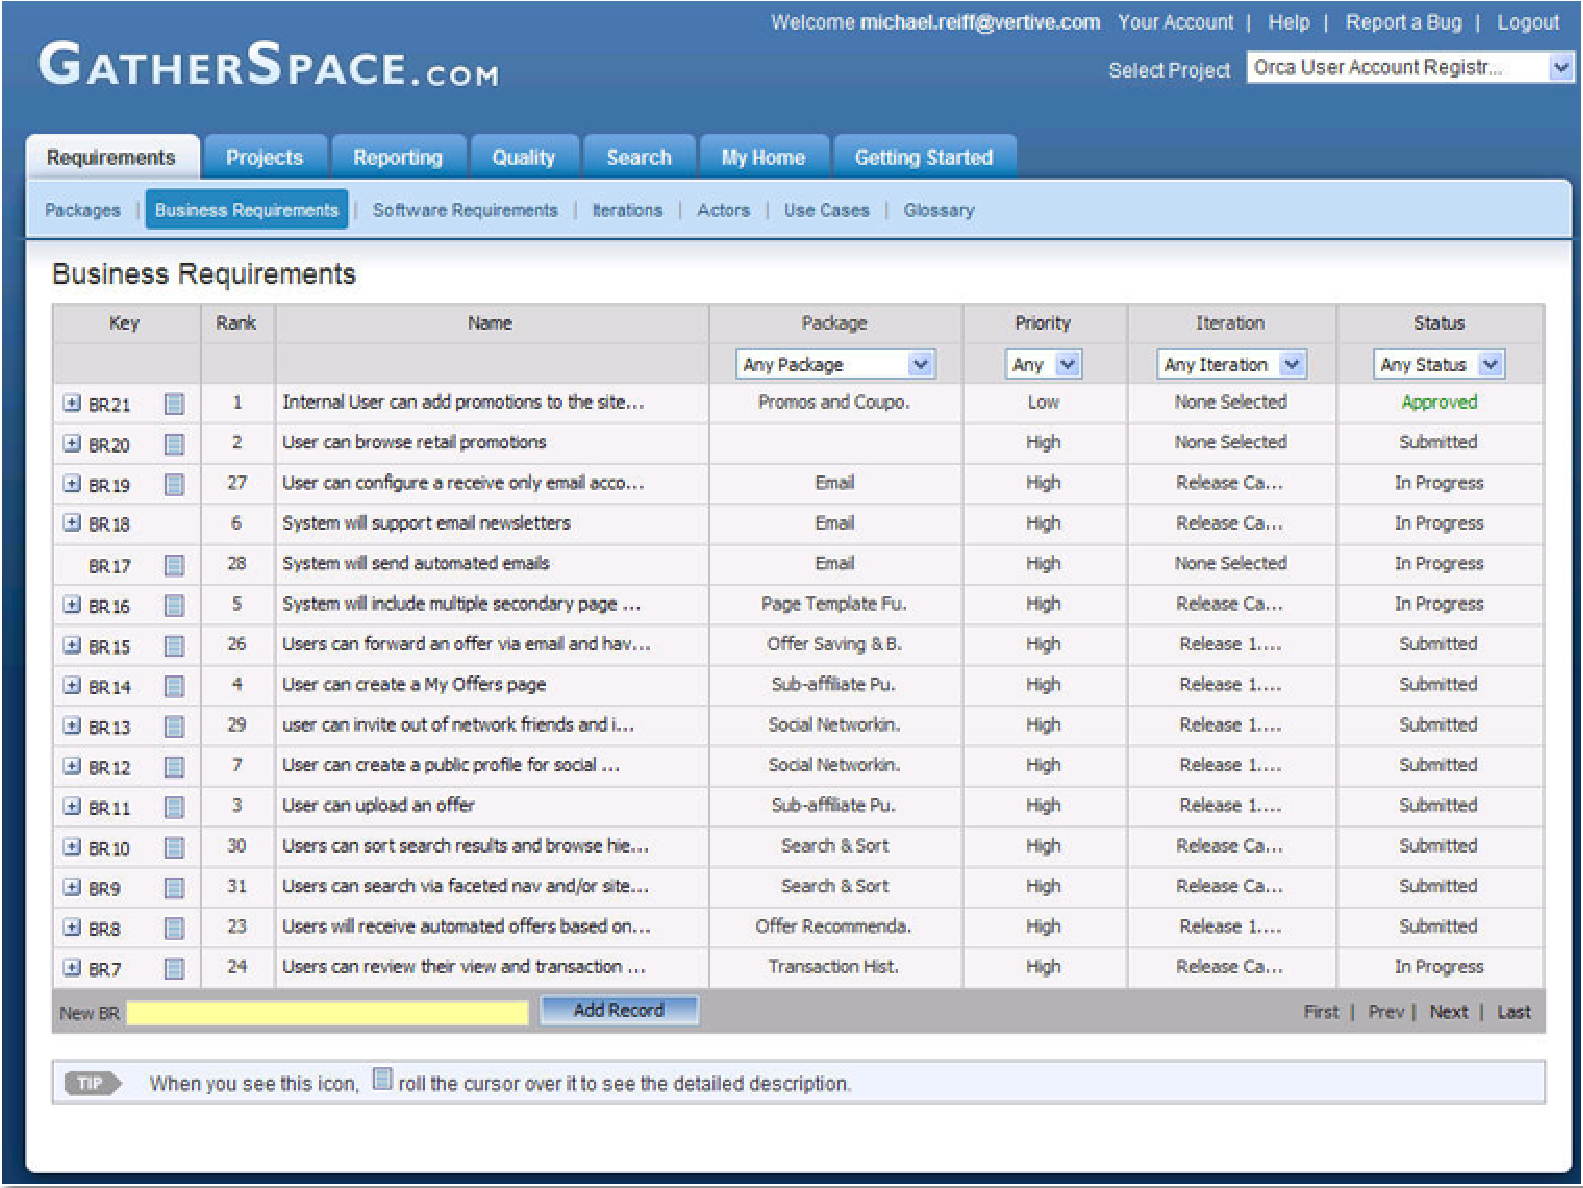
\includegraphics[width=1.0\textwidth]{img/gatherspace_1.pdf}
        \caption{Gatherspace.com - business requirements}
        \label{fig:gatherspace_1}
      \end{figure*}

      \begin{figure*}[t]
        \centering
        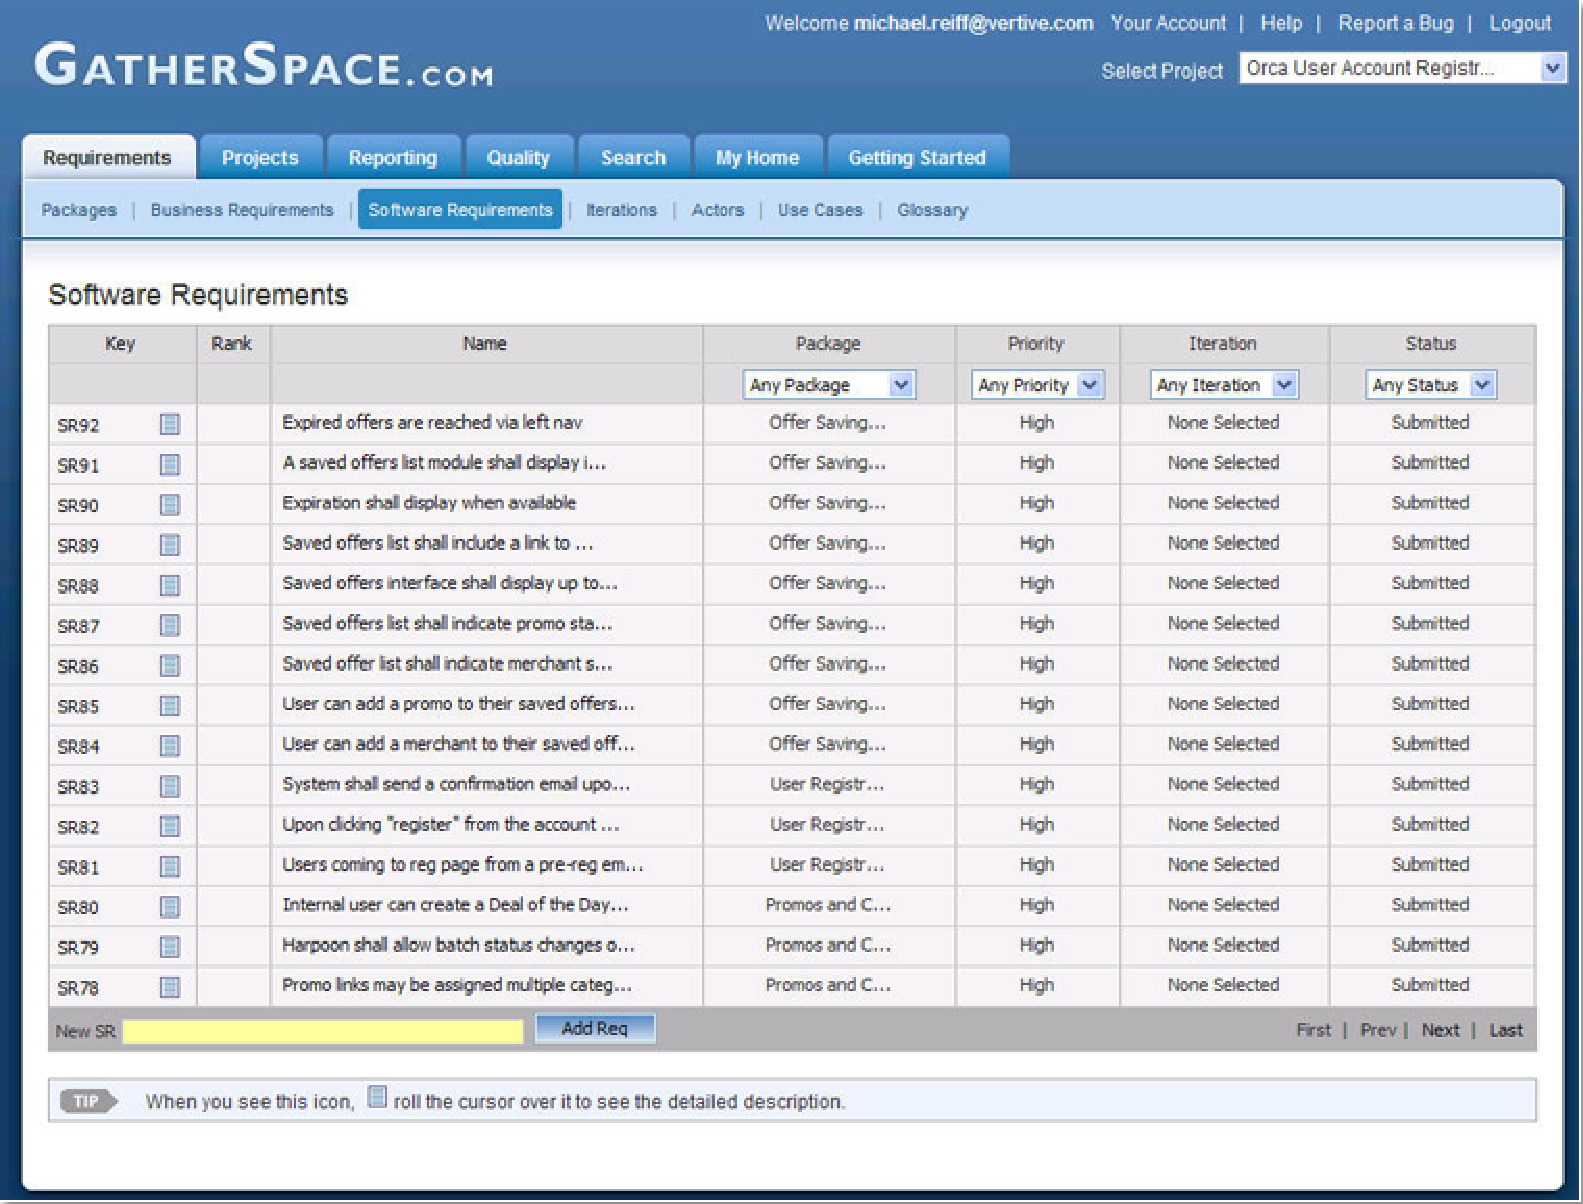
\includegraphics[width=1.0\textwidth]{img/gatherspace_2.pdf}
        \caption{Gatherspace.com - software requirements}
        \label{fig:gatherspace_2}
      \end{figure*}

      \begin{figure*}[t]
        \centering
        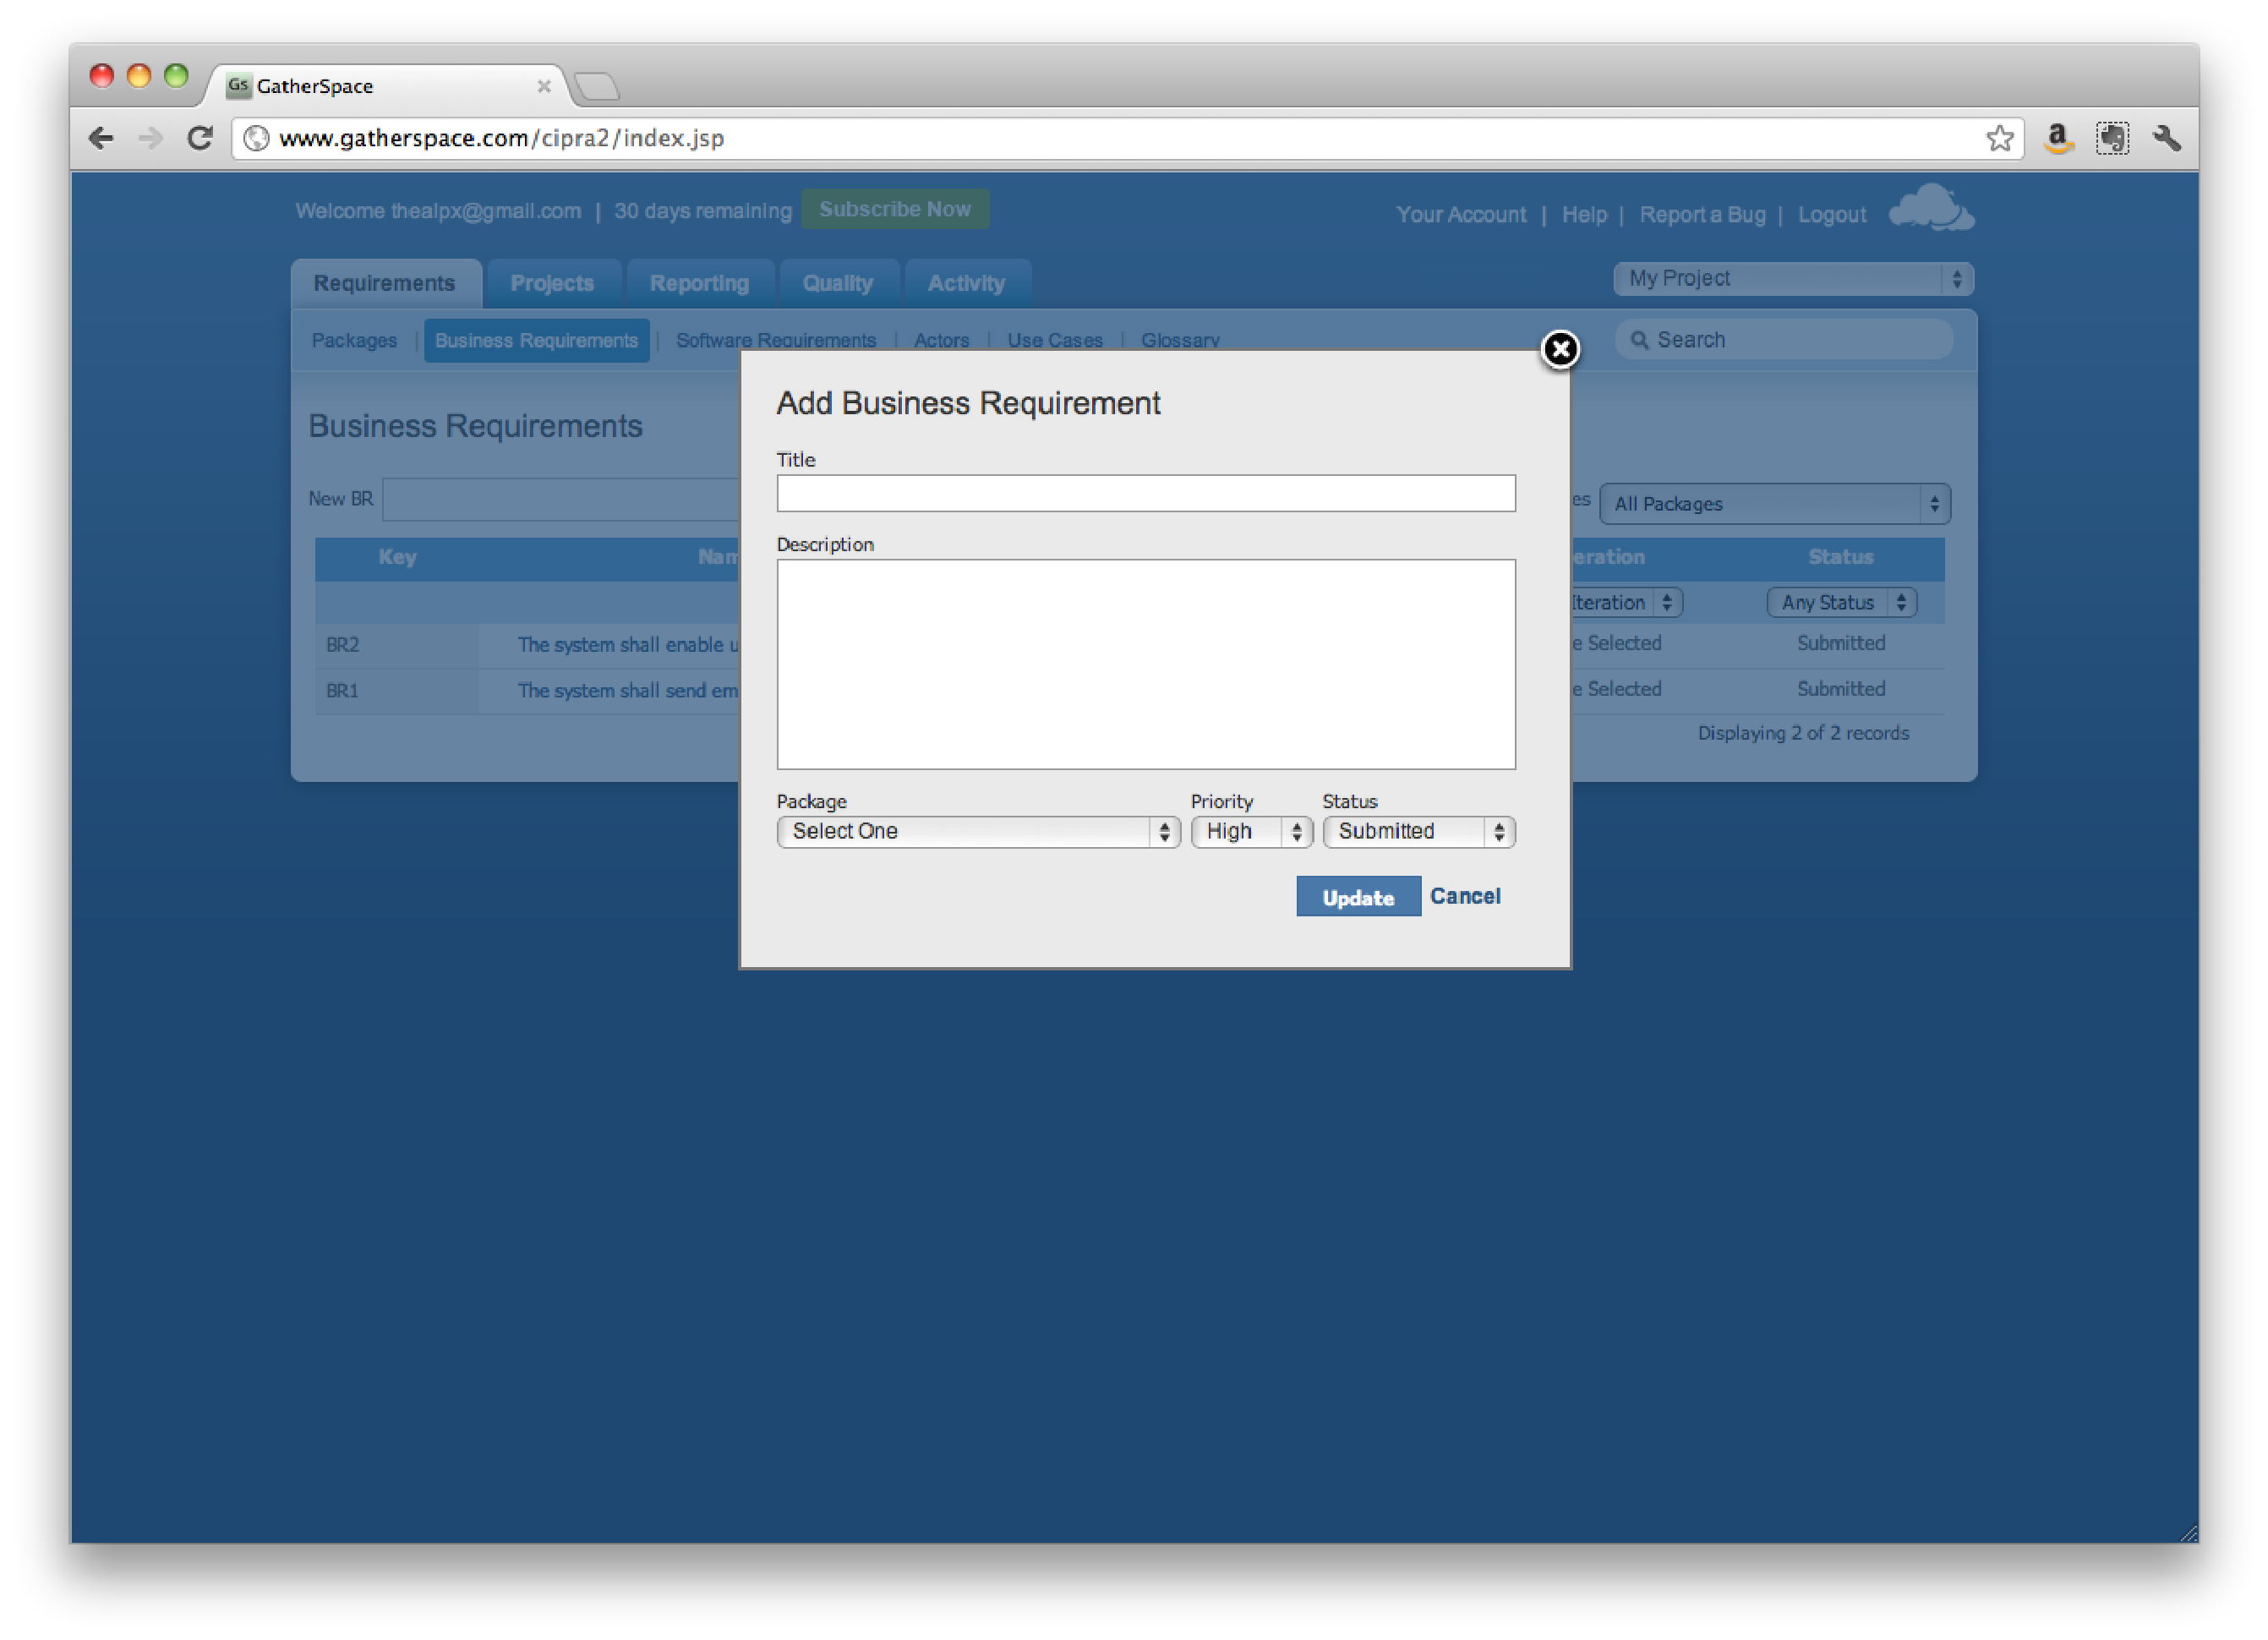
\includegraphics[width=1.0\textwidth]{img/gatherspace_5.pdf}
        \caption{Gatherspace.com - dodawanie wymagania ze szczegółami}
        \label{fig:gatherspace_5}
      \end{figure*}

      \begin{figure*}[t]
        \centering
        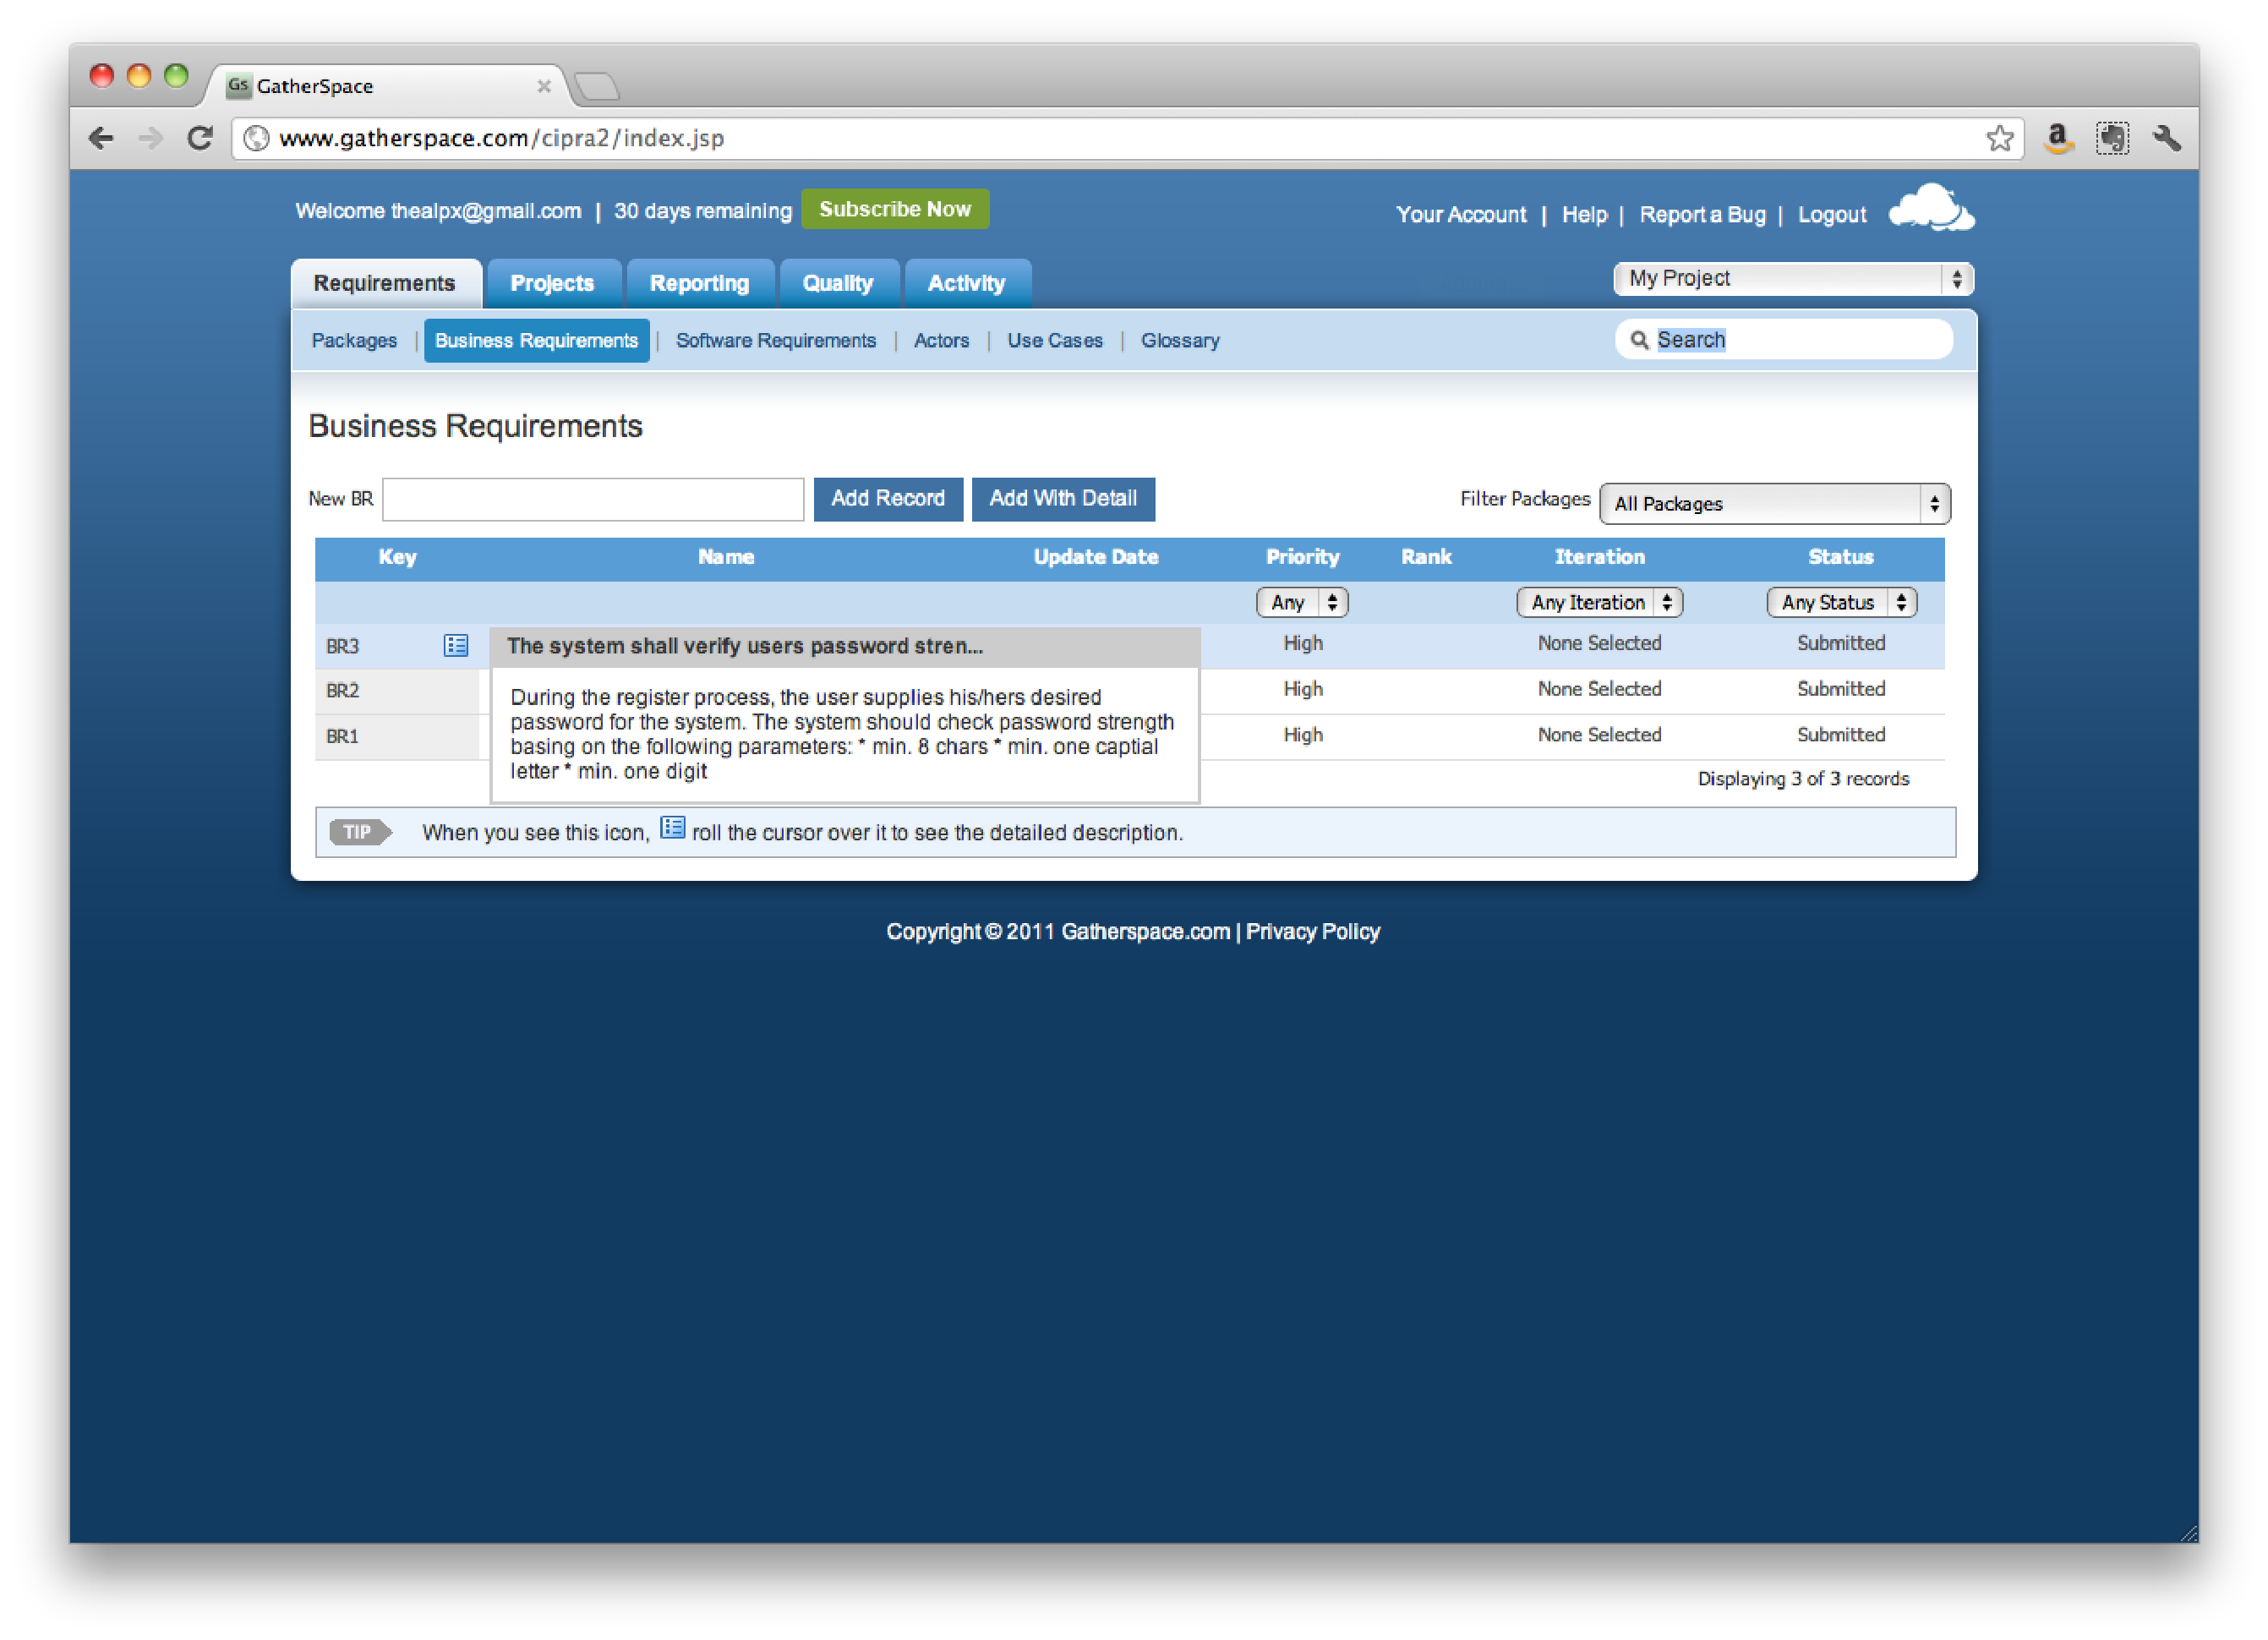
\includegraphics[width=1.0\textwidth]{img/gatherspace_6.pdf}
        \caption{Gatherspace.com - tooltip ze szczegółami wymagania}
        \label{fig:gatherspace_6}
      \end{figure*}

      \begin{figure*}[t]
        \centering
        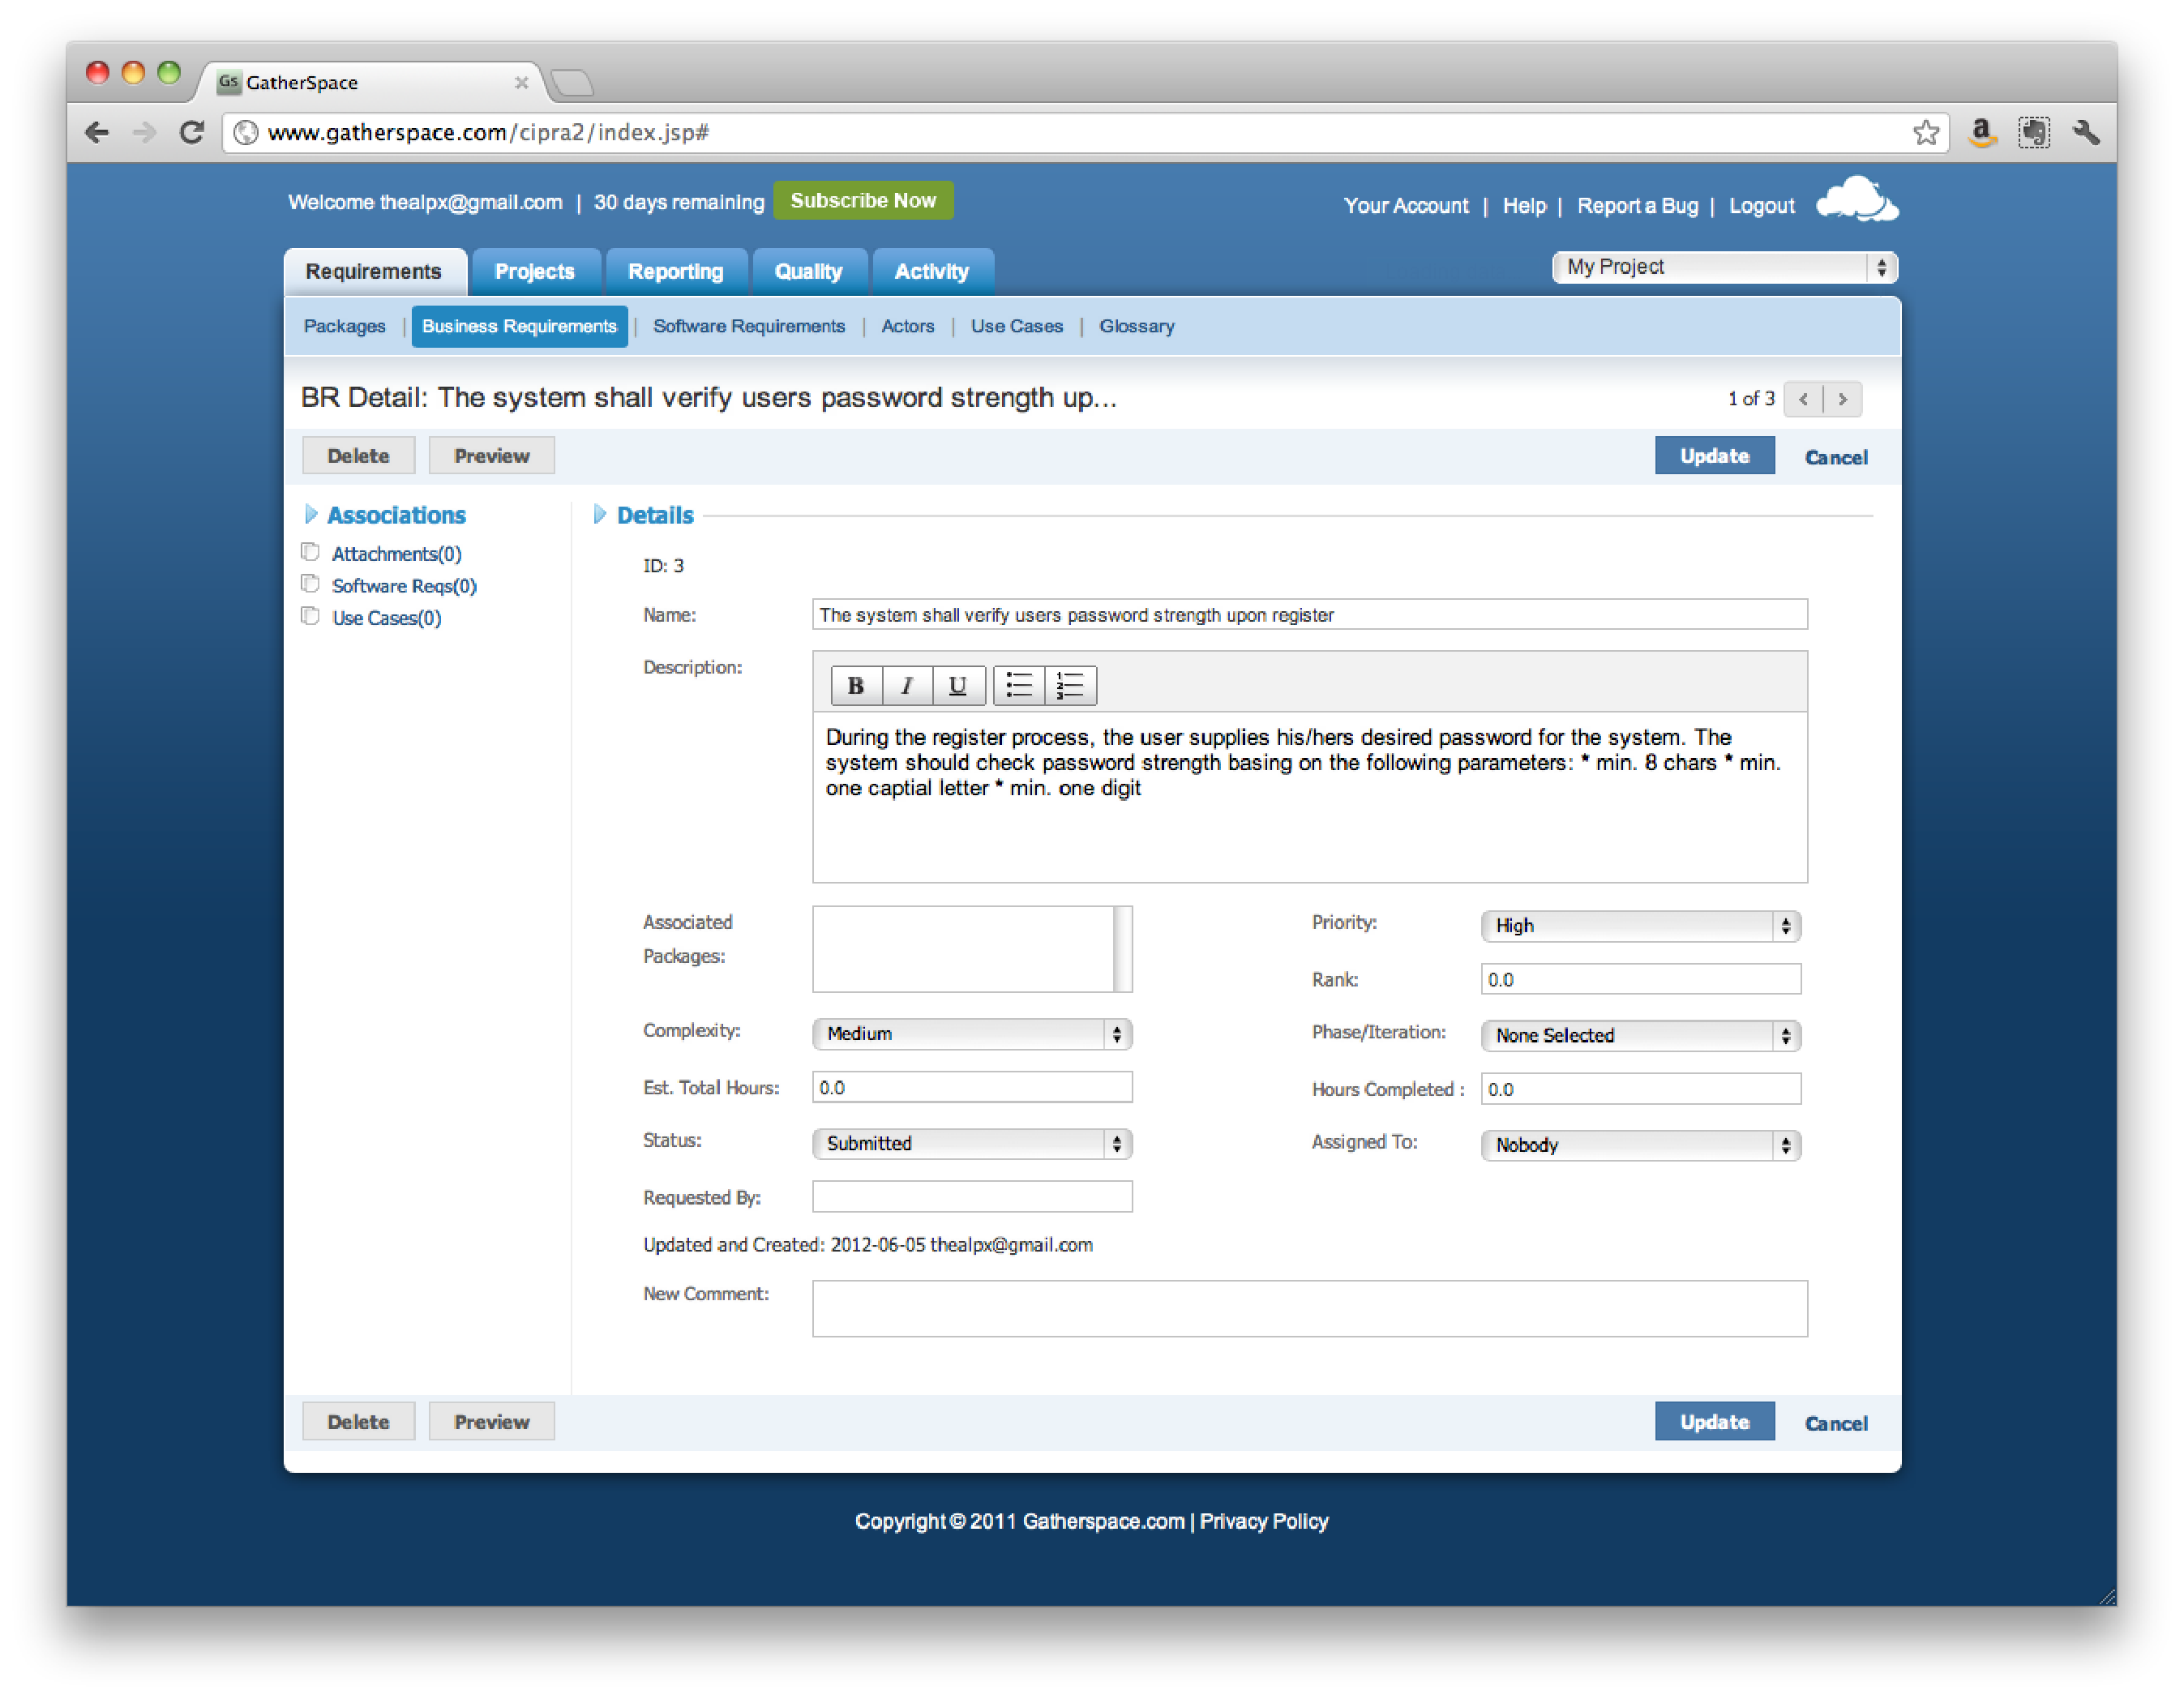
\includegraphics[width=1.0\textwidth]{img/gatherspace_7.pdf}
        \caption{Gatherspace.com - widok szczegółów wymagania}
        \label{fig:gatherspace_7}
      \end{figure*}

      \begin{figure*}[t]
        \centering
        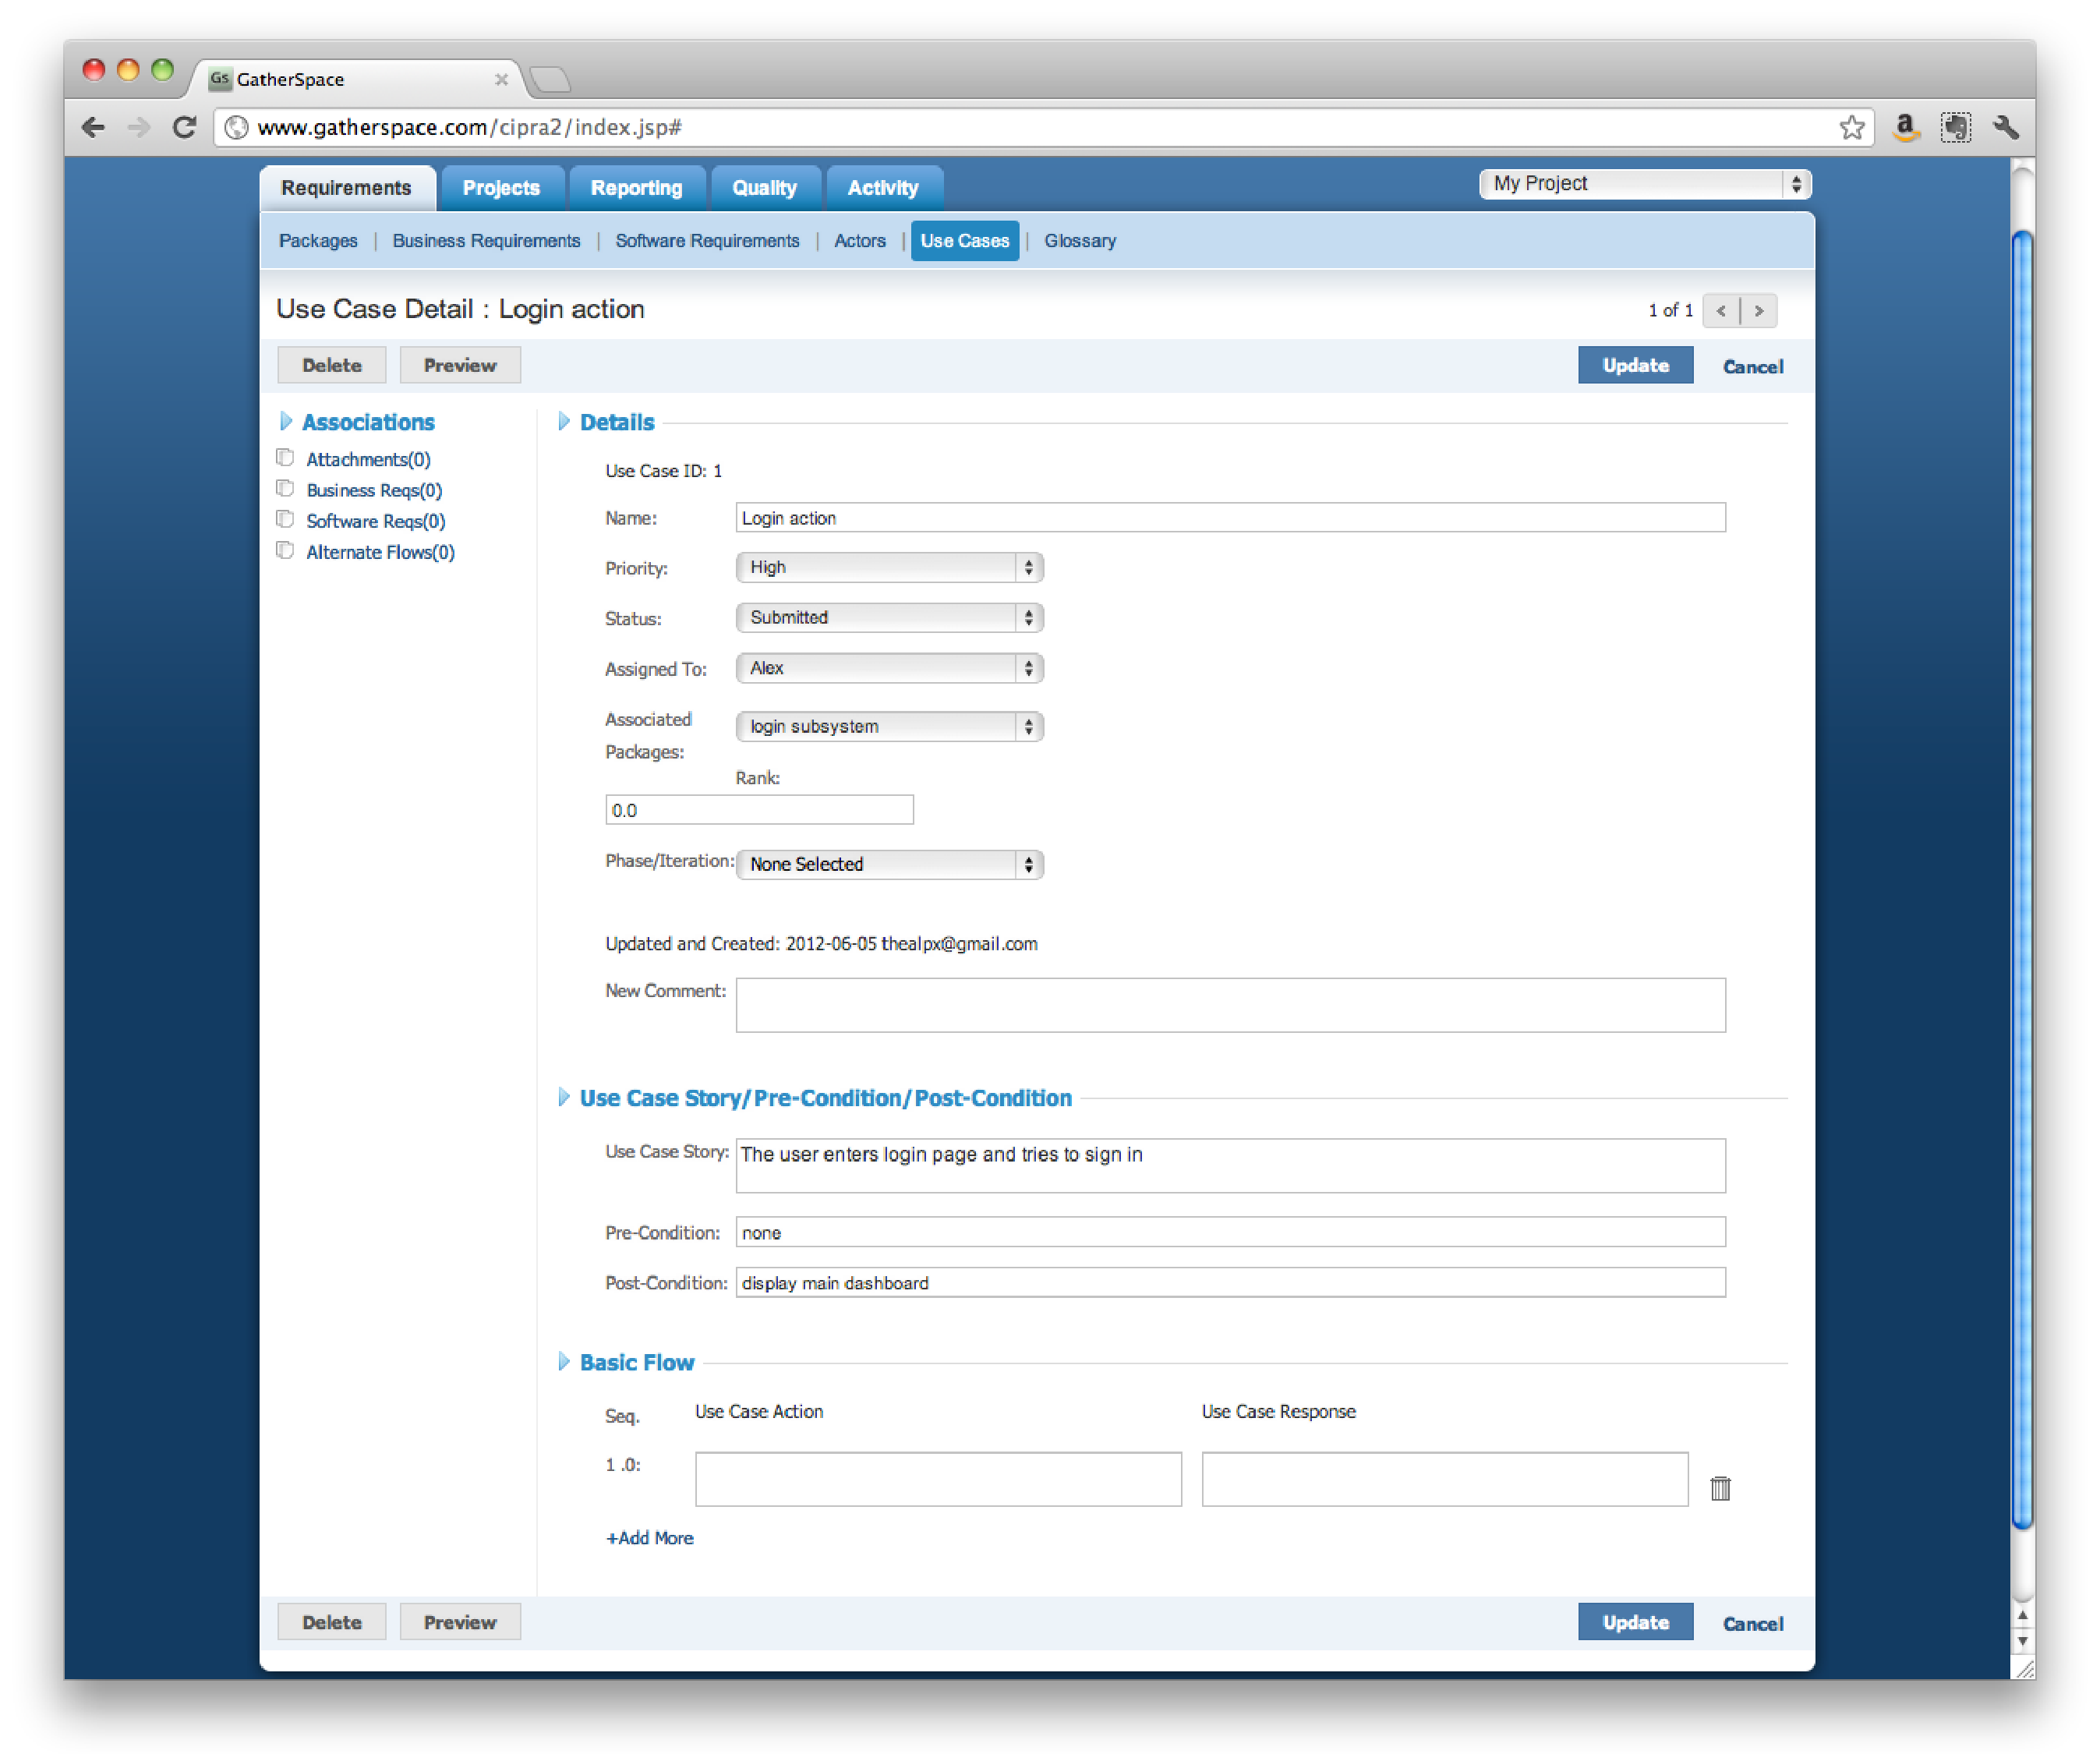
\includegraphics[width=1.0\textwidth]{img/gatherspace_8.pdf}
        \caption{Gatherspace.com - widok szczegółów wymagania}
        \label{fig:gatherspace_8}
      \end{figure*}

      \begin{figure*}[t]
        \centering
        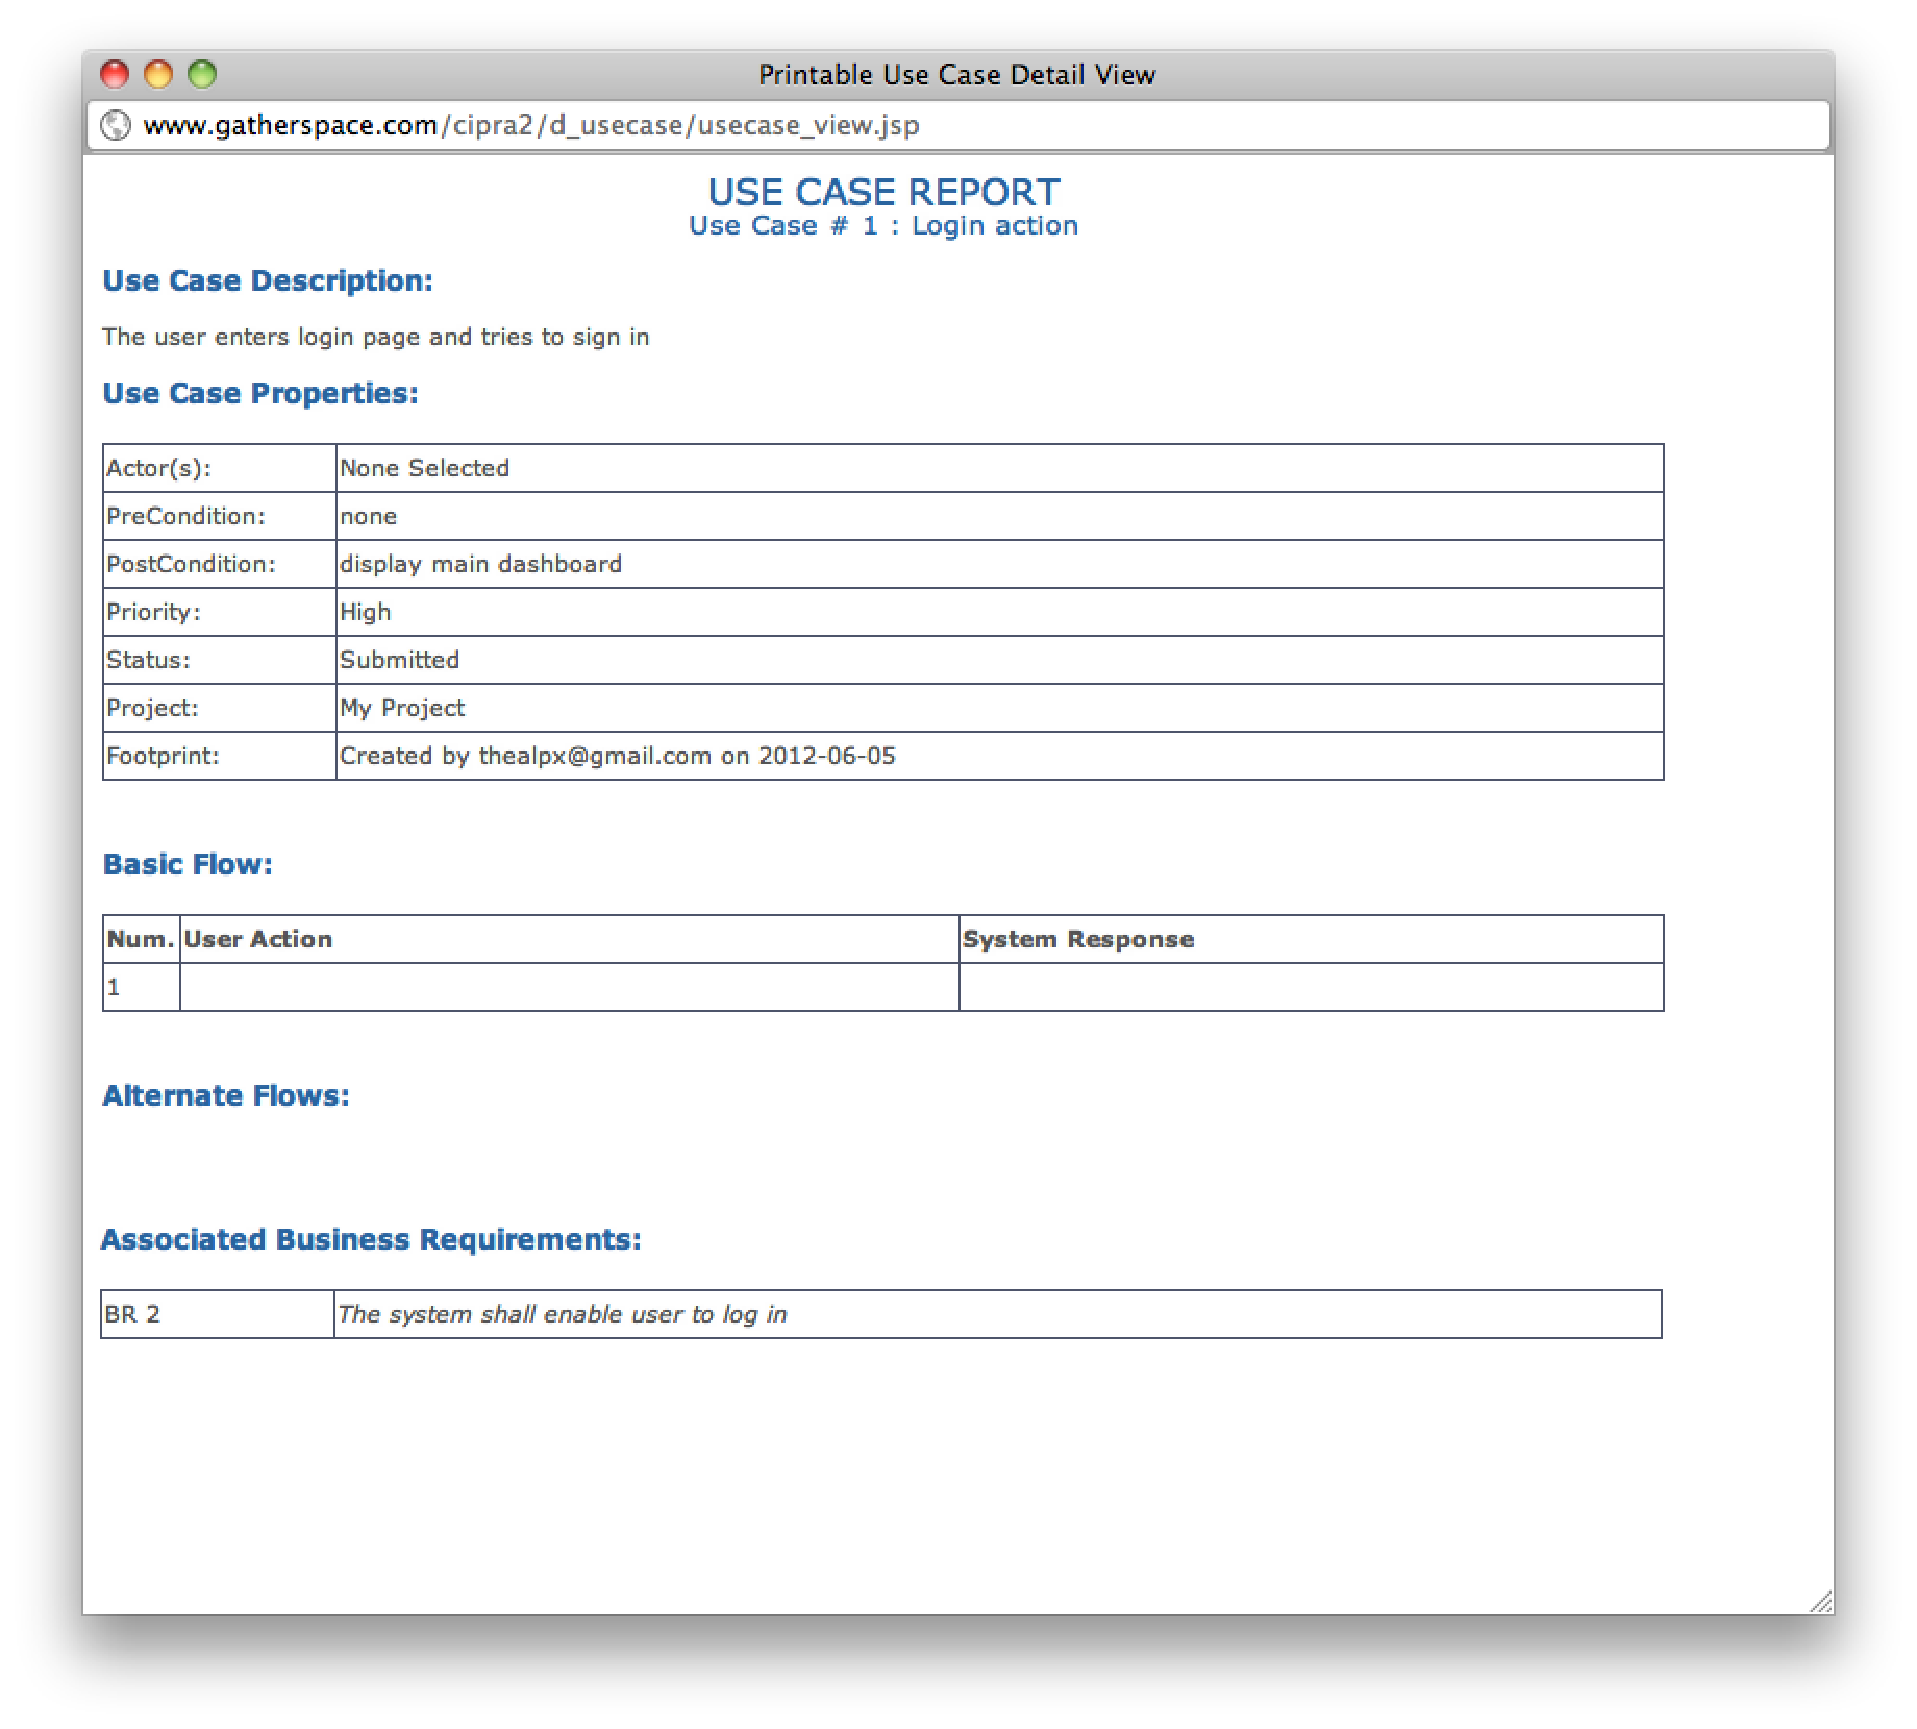
\includegraphics[width=1.0\textwidth]{img/gatherspace_9.pdf}
        \caption{Gatherspace.com - wymaganie przygotowane do druku}
        \label{fig:gatherspace_9}
      \end{figure*}

      \begin{figure*}[t]
        \centering
        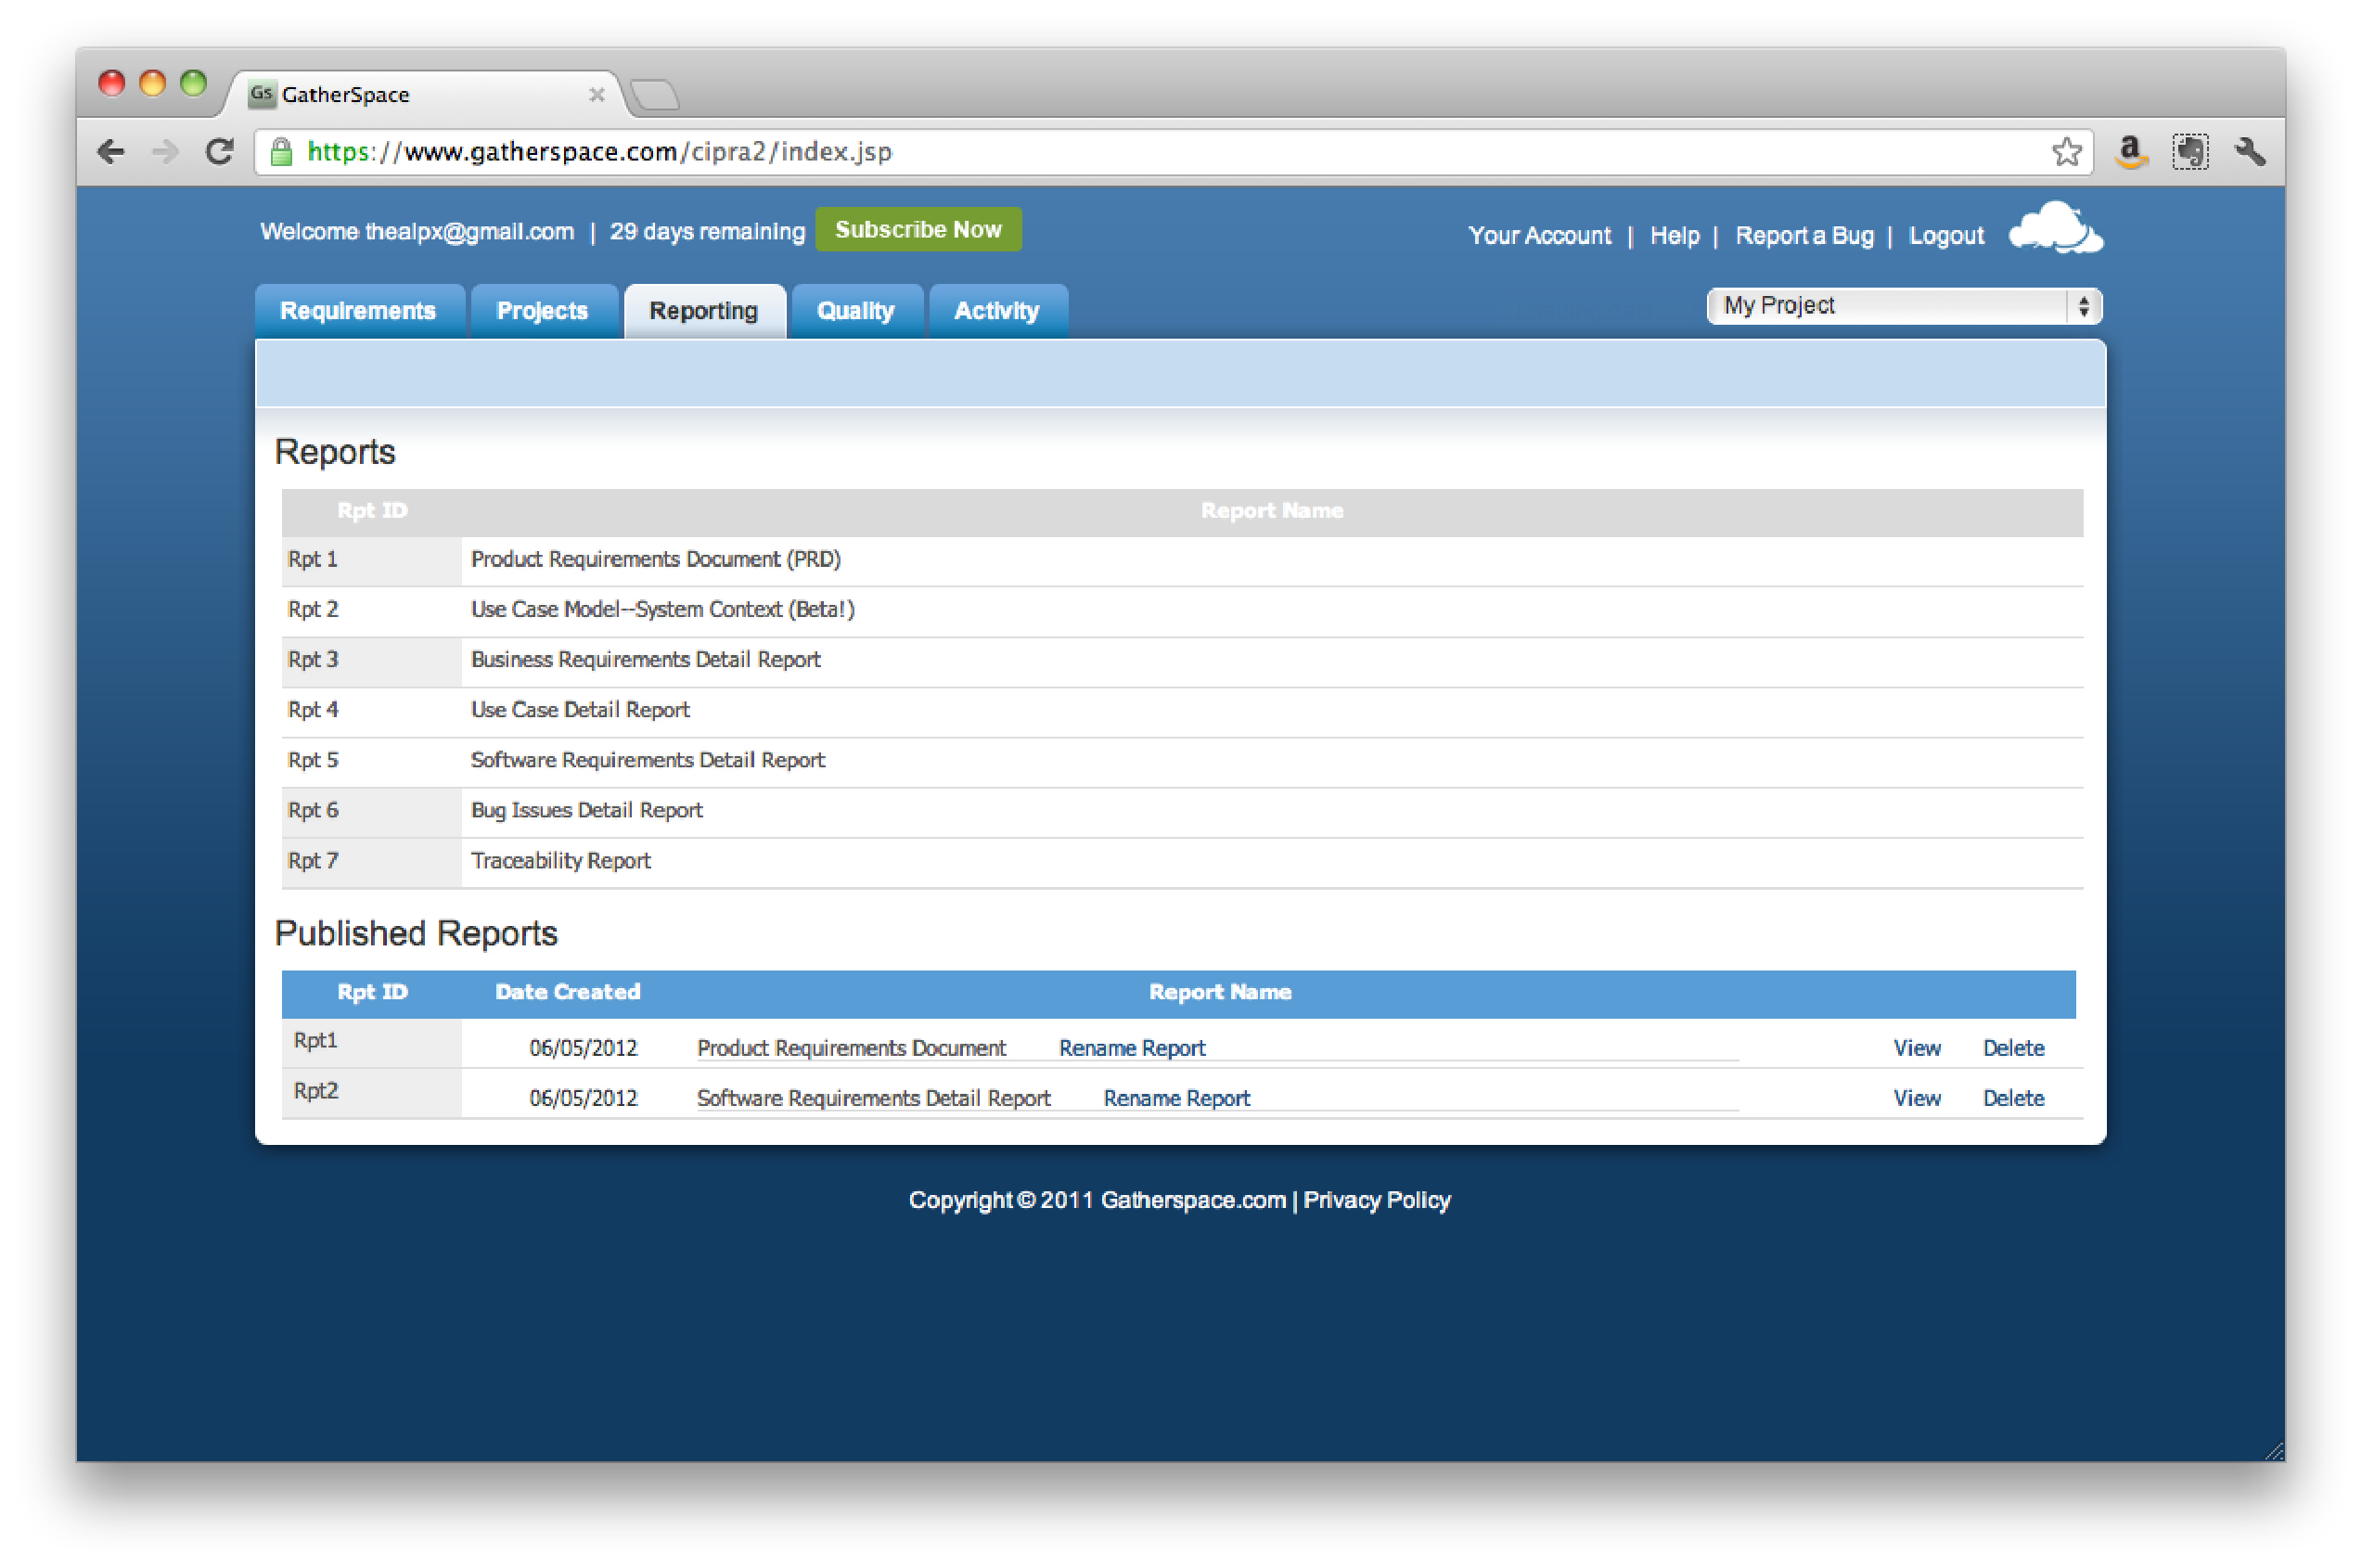
\includegraphics[width=1.0\textwidth]{img/gatherspace_11.pdf}
        \caption{Gatherspace.com - dostępne raporty}
        \label{fig:gatherspace_11}
      \end{figure*}

      \subsubsection{Gatherspace}
        Gatherspace dzieli wymagania na biznesowe (business requirements) oraz funkcjonalne (software requirements). Dostępne są osobne widoki dla obu typów wymagań (rys. \ref{fig:gatherspace_1}, \ref{fig:gatherspace_2}). Wymagania można katalogować w definiowane przez użytkownika pakiety, podobnie jak pliki w katalogach, w systemach operacyjnych. 


        Na rysunku \ref{fig:gatherspace_2} przedstawiono widok wymagań funkcjonalnych. Dodawanie wymagań przebiega w prosty sposób. Po wpisaniu tytułu wymagania i zatwierdzeniu pola formularza, element zostaje dodany do listy bez przeładowania strony.

        Wymaganie może zostać dodane na dwa sposoby - podając jedynie tytuł lub wybierając opcję ,,Add with detail''. Wówczas pojawia się ,,popup'' umożliwiający dodanie zarówno treści jak i opisu wymagania (patrz rys. \ref{fig:gatherspace_5}).

        Wymaganie posiadające opis, zaopatrzone jest w specjalną ikonkę po lewej stronie. Użytkownik wskazujący w to miejsce myszką może podejrzeć treść wymagania, bez konieczności otwierania jego szczegółów. Jest to dość przydatna funkcjonalność, pozwalająca szybko zapoznać się pobieżnie z danym wymaganiem. Rysunek \ref{fig:gatherspace_6} zawiera zrzut ekraniu prezentujący tę funkcjonalność. 
        
        Widok szczegółów wymagania jest dość prosty i przejrzysty (rys. \ref{fig:gatherspace_7}). Do dyspozycji użytkownika jest formularz zawierający pola z parametrami wymagania, takimi jak m.in.: priorytet, status, poziom złożoności, pakiet do którego należy, przez kogo wymaganie zostało dodane oraz kto lub co jest źródłem wymagania.

        Dodawanie przypadków użycia jest wydzielone do osobnego widoku i funkcjonuje jako osobny zestaw formularzy (rys. \ref{fig:gatherspace_8}). 

        Istnieje możliwość łączenia przypadków użycia z wymaganiami poprzez wskazanie konkretnego wymagania w osobnym widoku, jednak system nie umożliwia łączenia tych artefaktów z poziomu edytora graficznego.

        Zarówno przypadki użycia jak i wymagania mogą zostać wyświetlone w formie przyjaznej do druku. Dla przykładu zamieszczono zrzut ekranu obrazujący jeden przypadek użycia przygotowany do druku na rys. \ref{fig:gatherspace_9}

        Dostępne w systemie raporty umożliwiają wyświetlenie i wydruk raportów dotyczących wymagań funkcjonalnych i niefunkcjonalnych, raport przypadków użycia oraz raport identyfikowalności (traceability report), umożliwiający przeanalizowanie związków pomiędzy wymaganiami a przypadkami użycia (patrz rysunek \ref{fig:gatherspace_11}). 

        \pagebreak

        Koszt zakupu licencji na oprogramowanie Gatherspace to minimum 19\$ za miesiąc użytkowania. Co ciekawe, istnieje możliwość zakupu wersji oprogramowania, które zostanie zainstalowane w infrastrukturze klienta. Jest to interesujące rozwiązanie dla klientów korporacyjnych, dla których przechowywanie danych na zewnętrznych serwerach jest wykluczone z powodów bezpieczeństwa (np. banki). Jednak koszt zakupu takiej licencji, jak można przeczytać na stronie gatherspace, to 4900\$ za instalację systemu. Dodatkowo firma żąda 295\$ miesięcznie za obsługę systemu. Biorąc pod uwagę zakres funkcjonalności oraz użyteczność systemu, są to ogromne kwoty, przewyższające, w ocenie autora, wartość dodaną wniesioną do organizacji wraz z wdrożeniem systemu Gatherspace.
         
        \begin{figure*}[t]
          \centering
          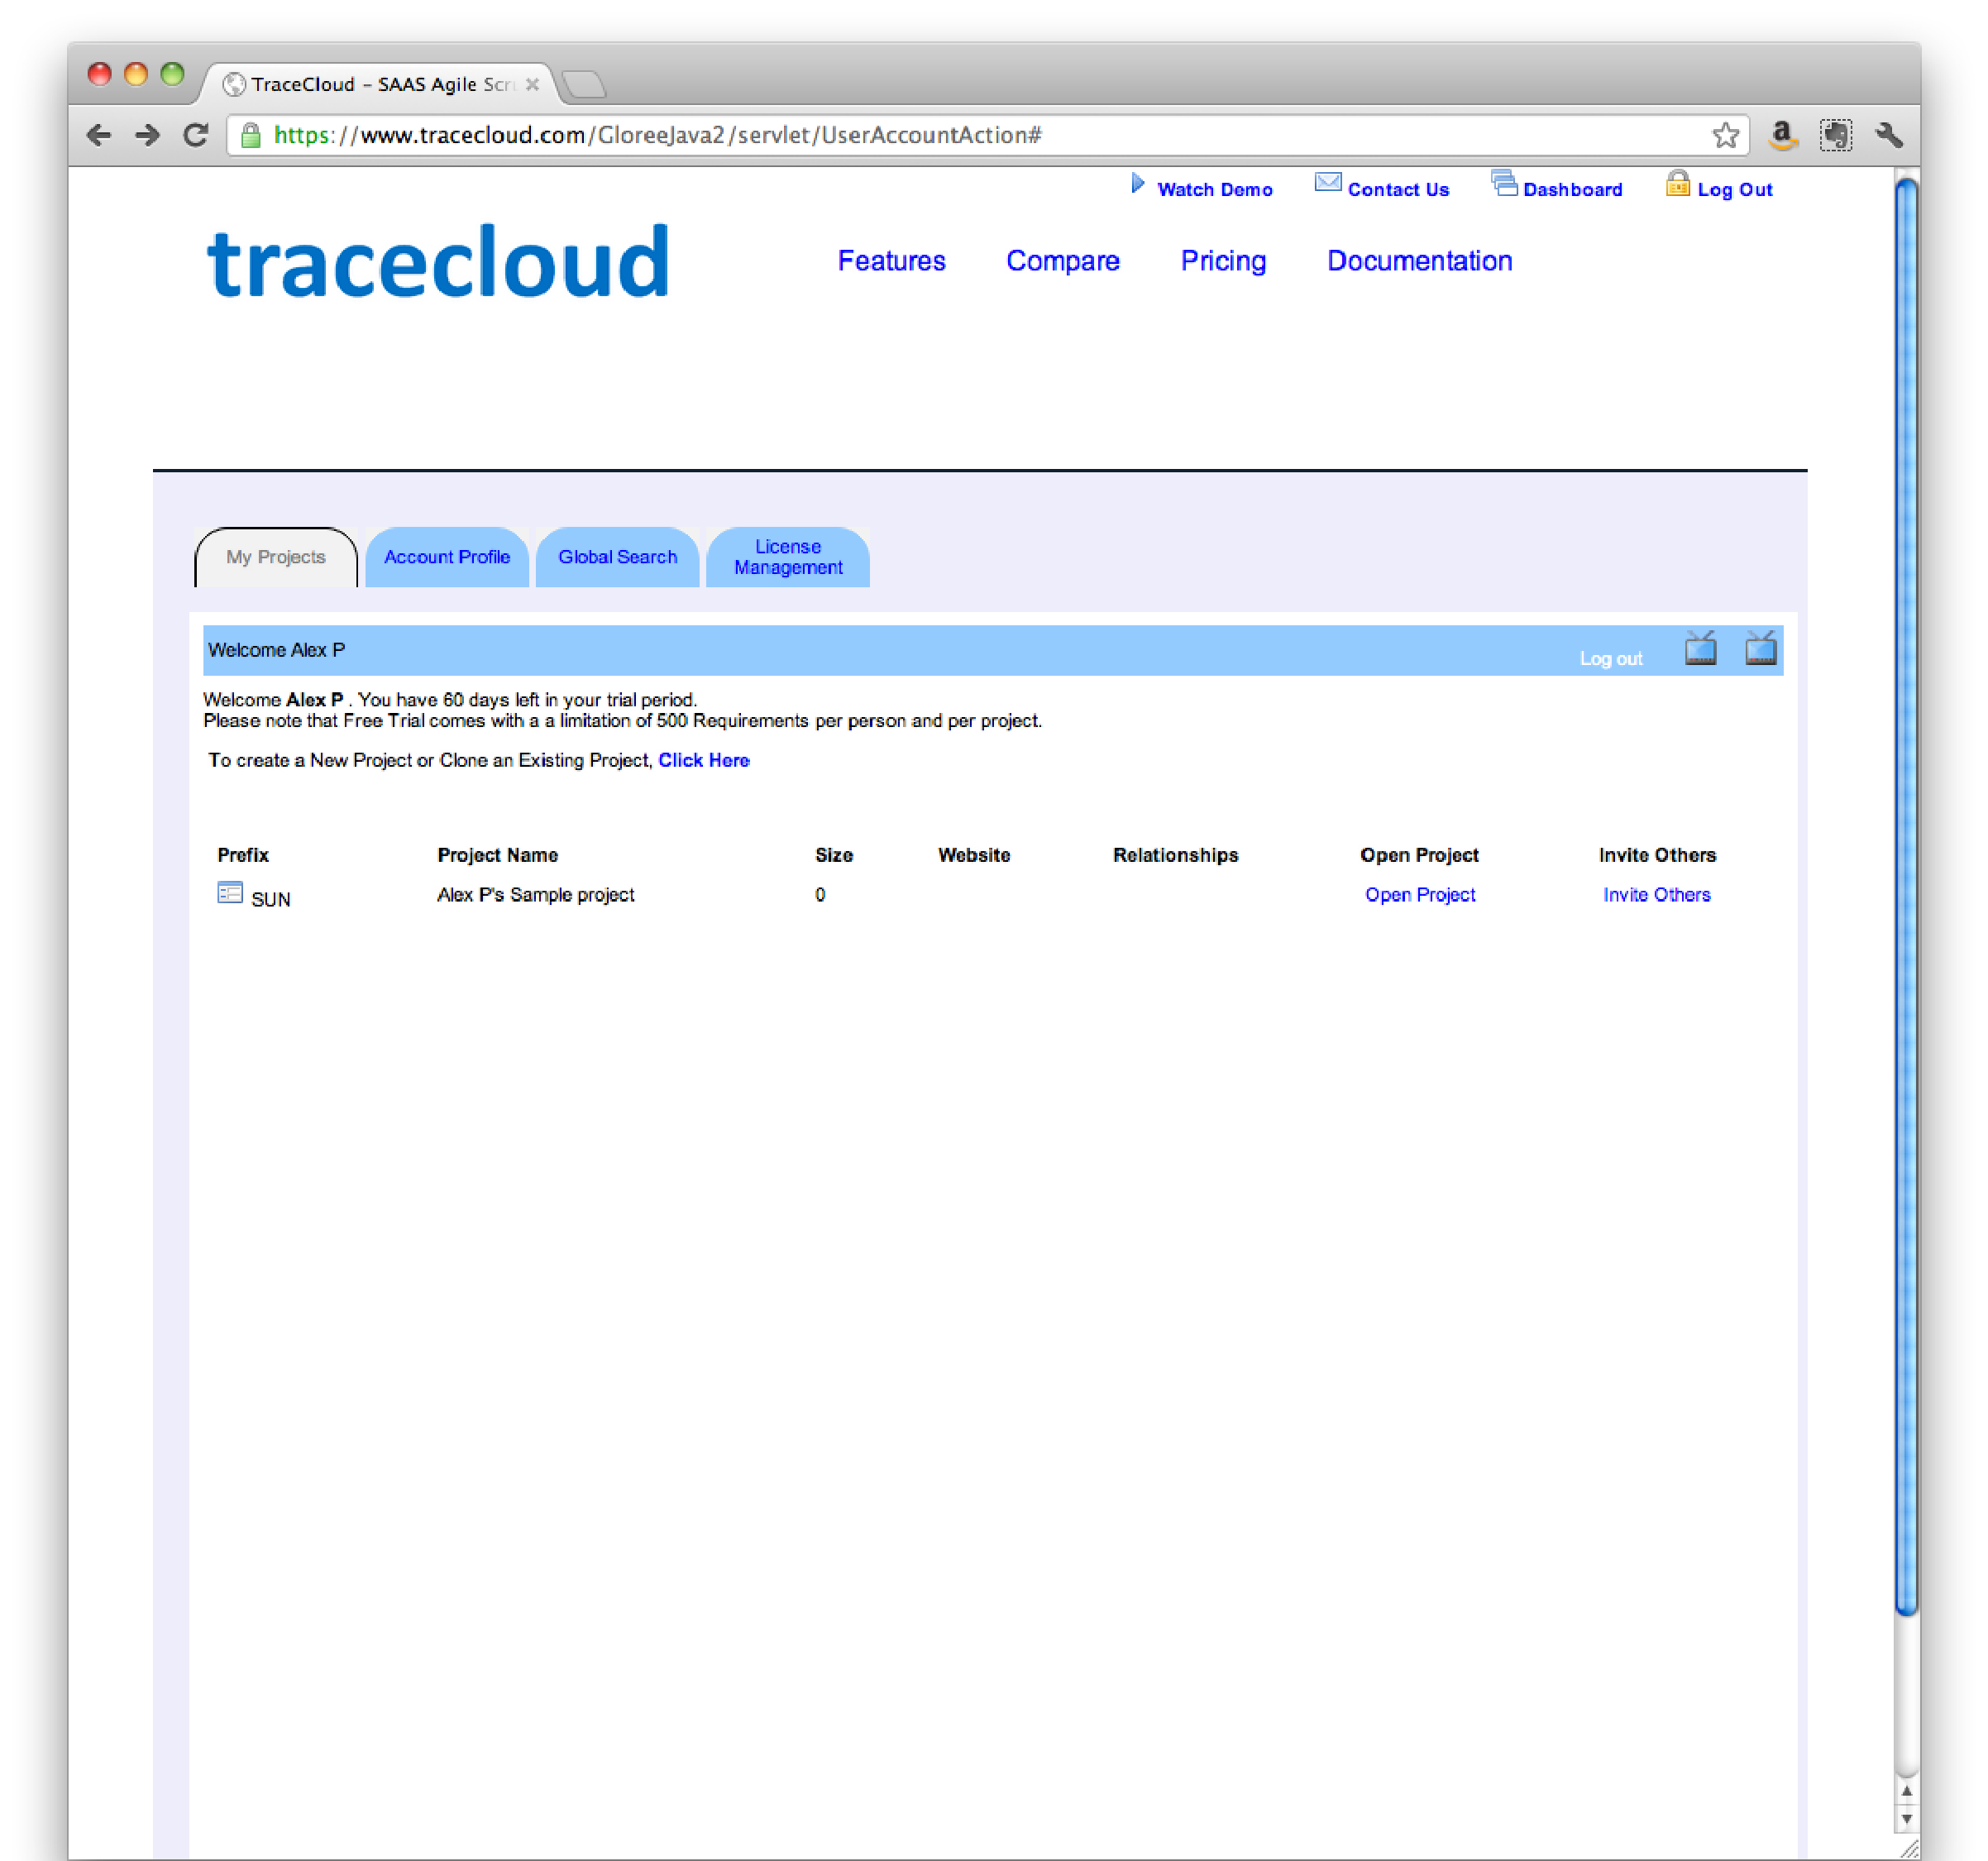
\includegraphics[width=1.0\textwidth]{img/tracecloud_1.pdf}
          \caption{Tracecloud - widok listy projektów}
          \label{fig:tracecloud_1}
        \end{figure*}

        \begin{figure*}[t]
          \centering
          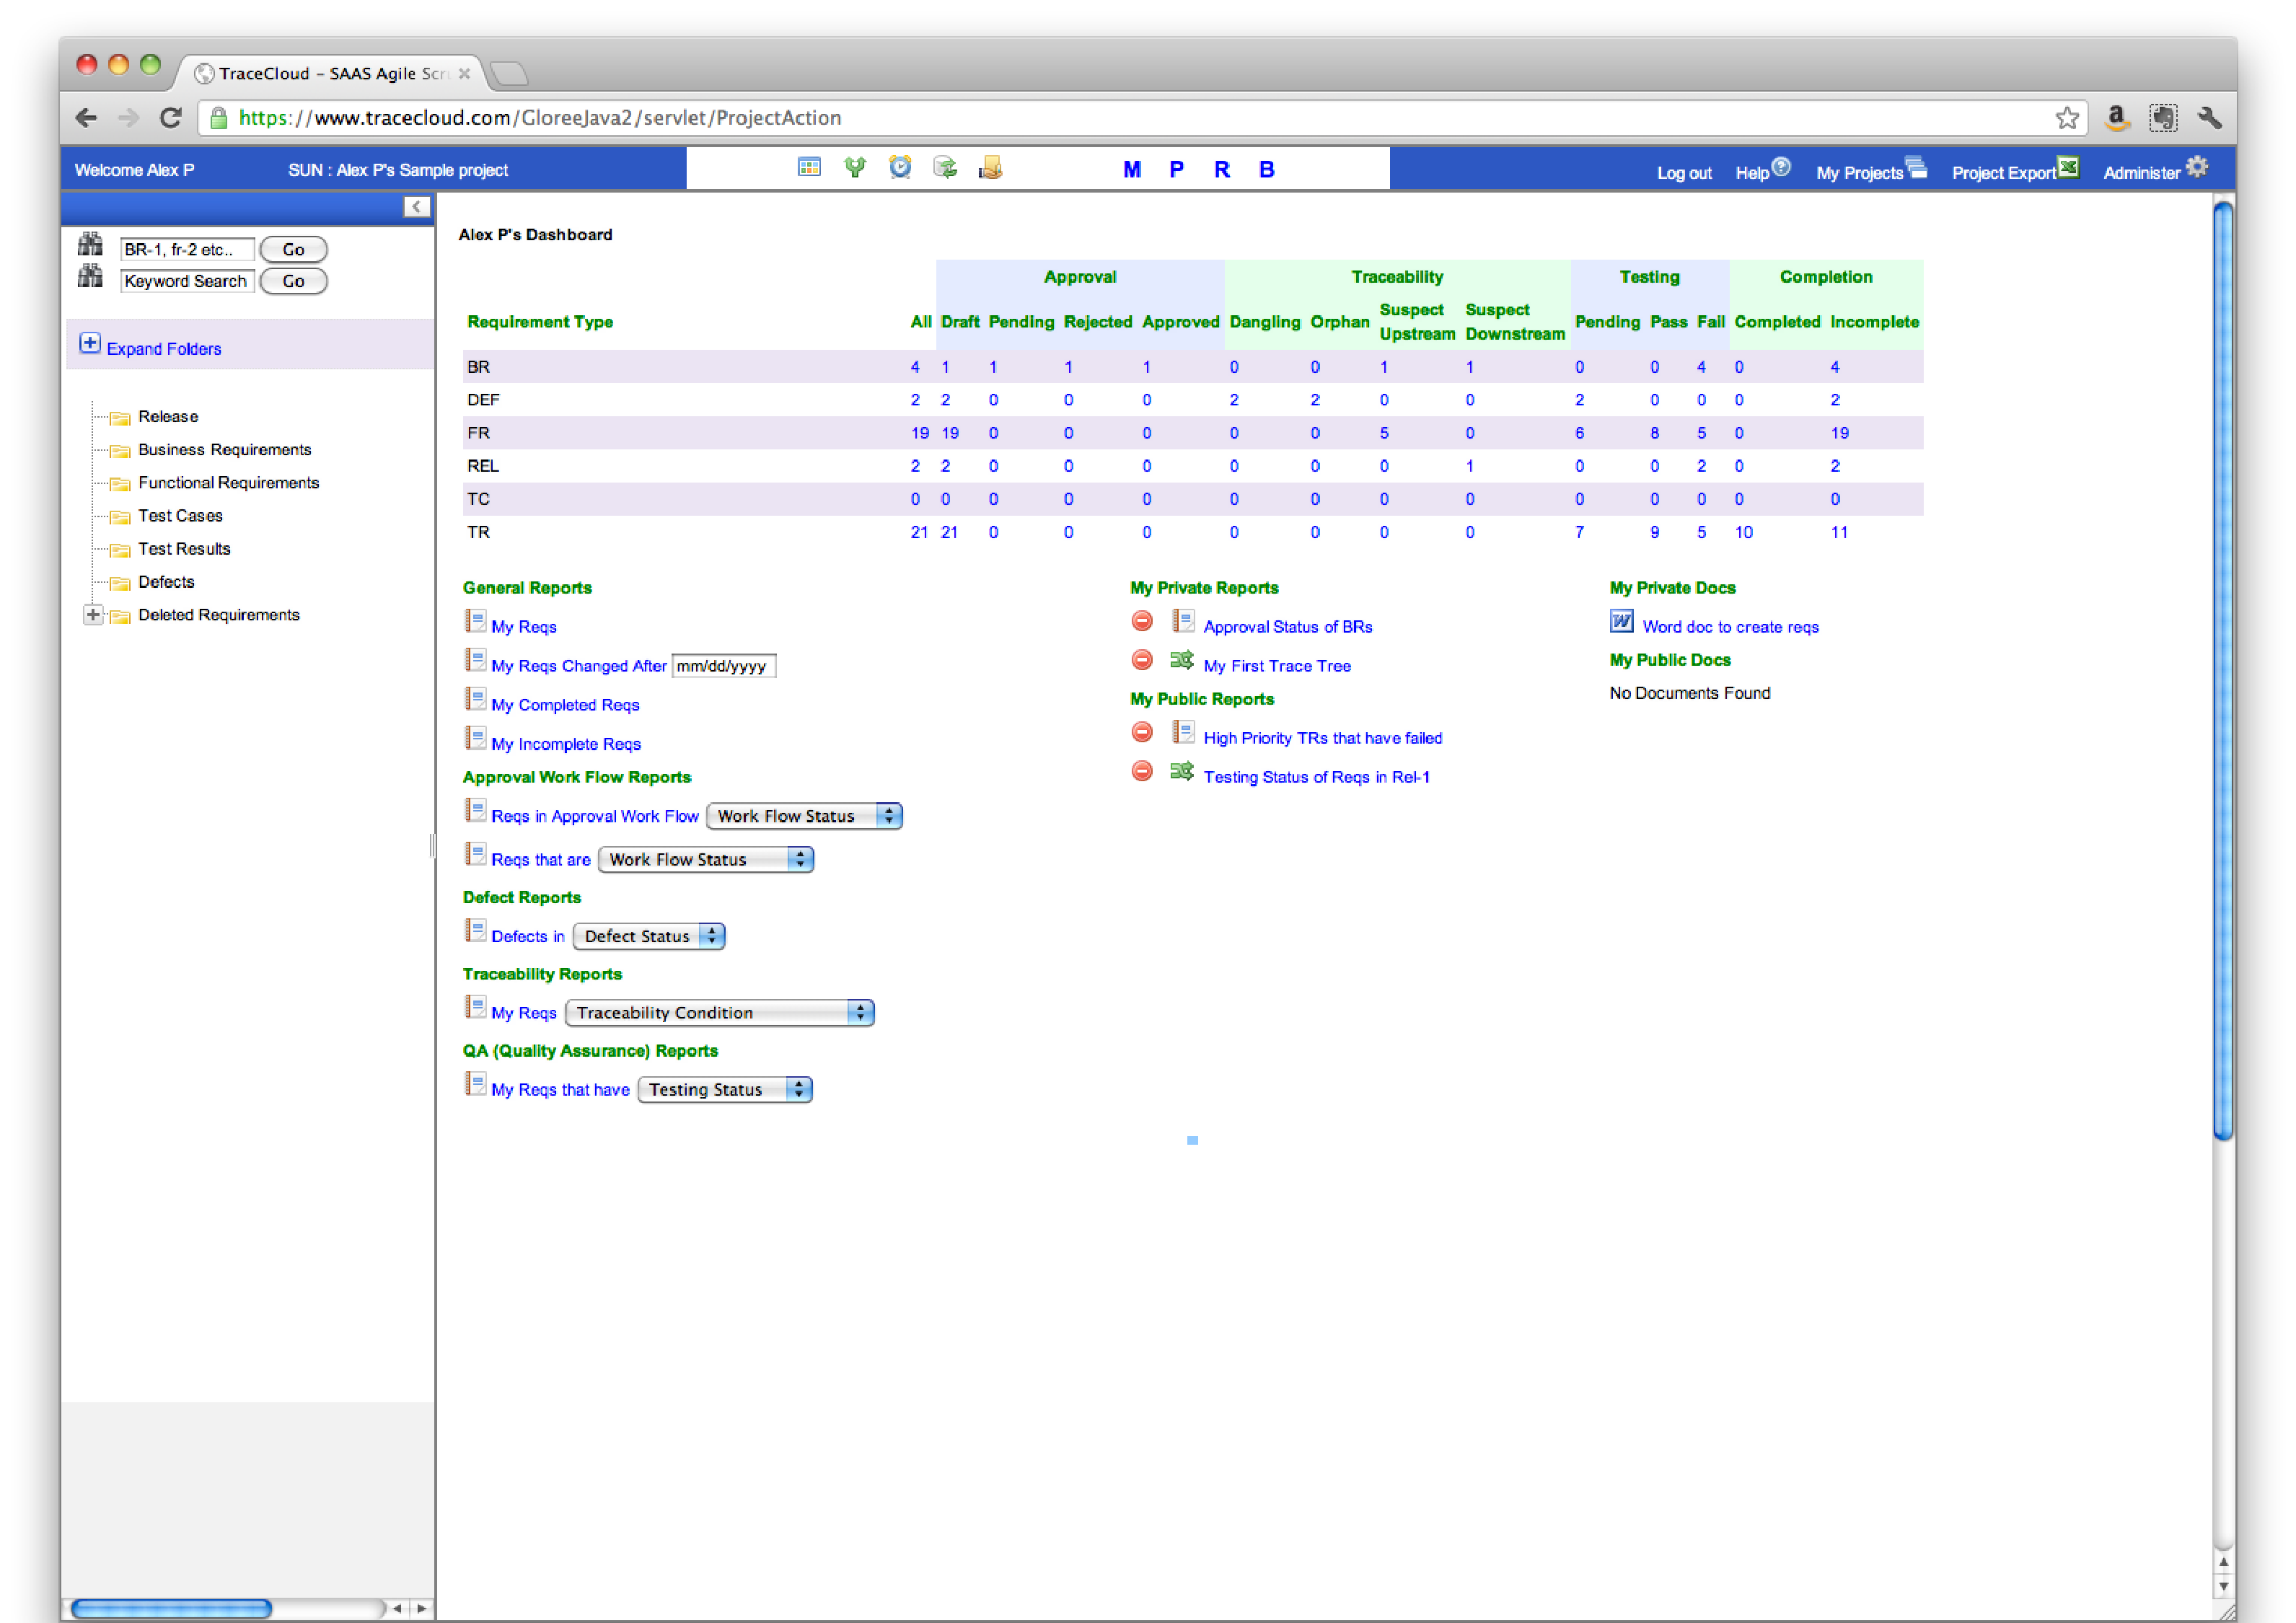
\includegraphics[width=1.0\textwidth]{img/tracecloud_2.pdf}
          \caption{Tracecloud - ekran główny}
          \label{fig:tracecloud_2}
        \end{figure*}

        \begin{figure*}[t]
          \centering
          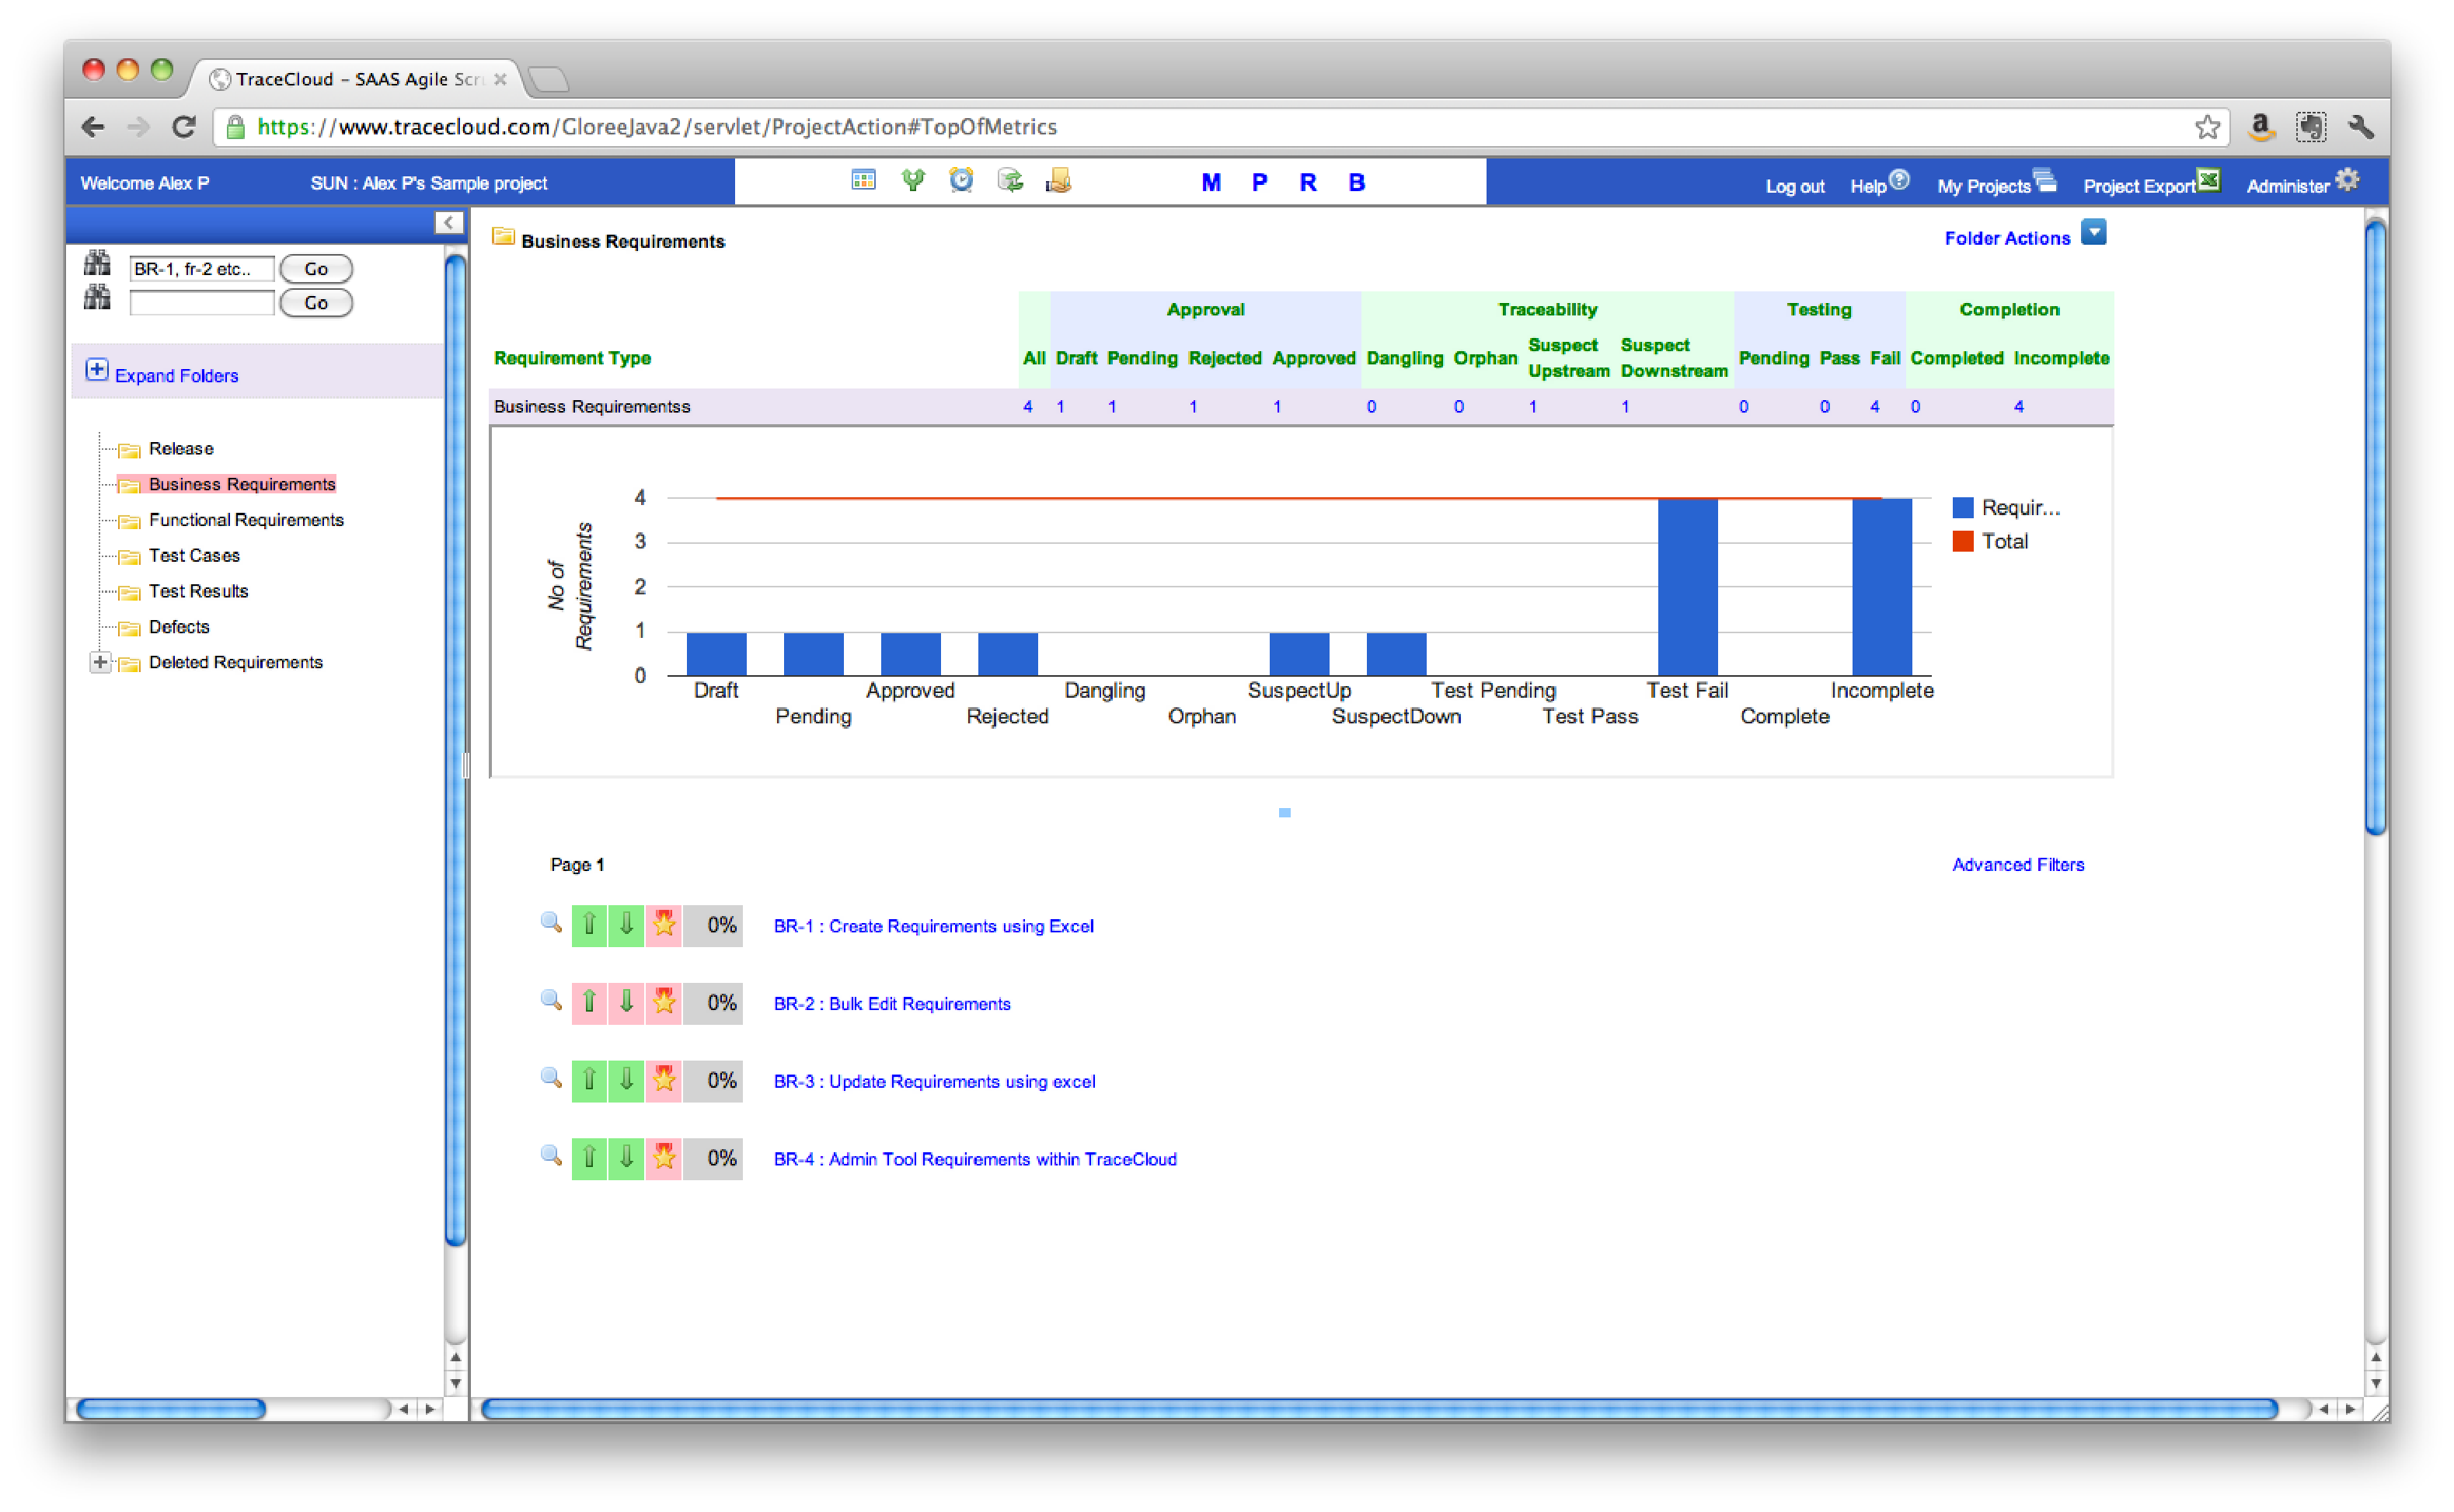
\includegraphics[width=1.0\textwidth]{img/tracecloud_3.pdf}
          \caption{Tracecloud - przegląd wymagań}
          \label{fig:tracecloud_3}
        \end{figure*}

        \begin{figure*}[t]
          \centering
          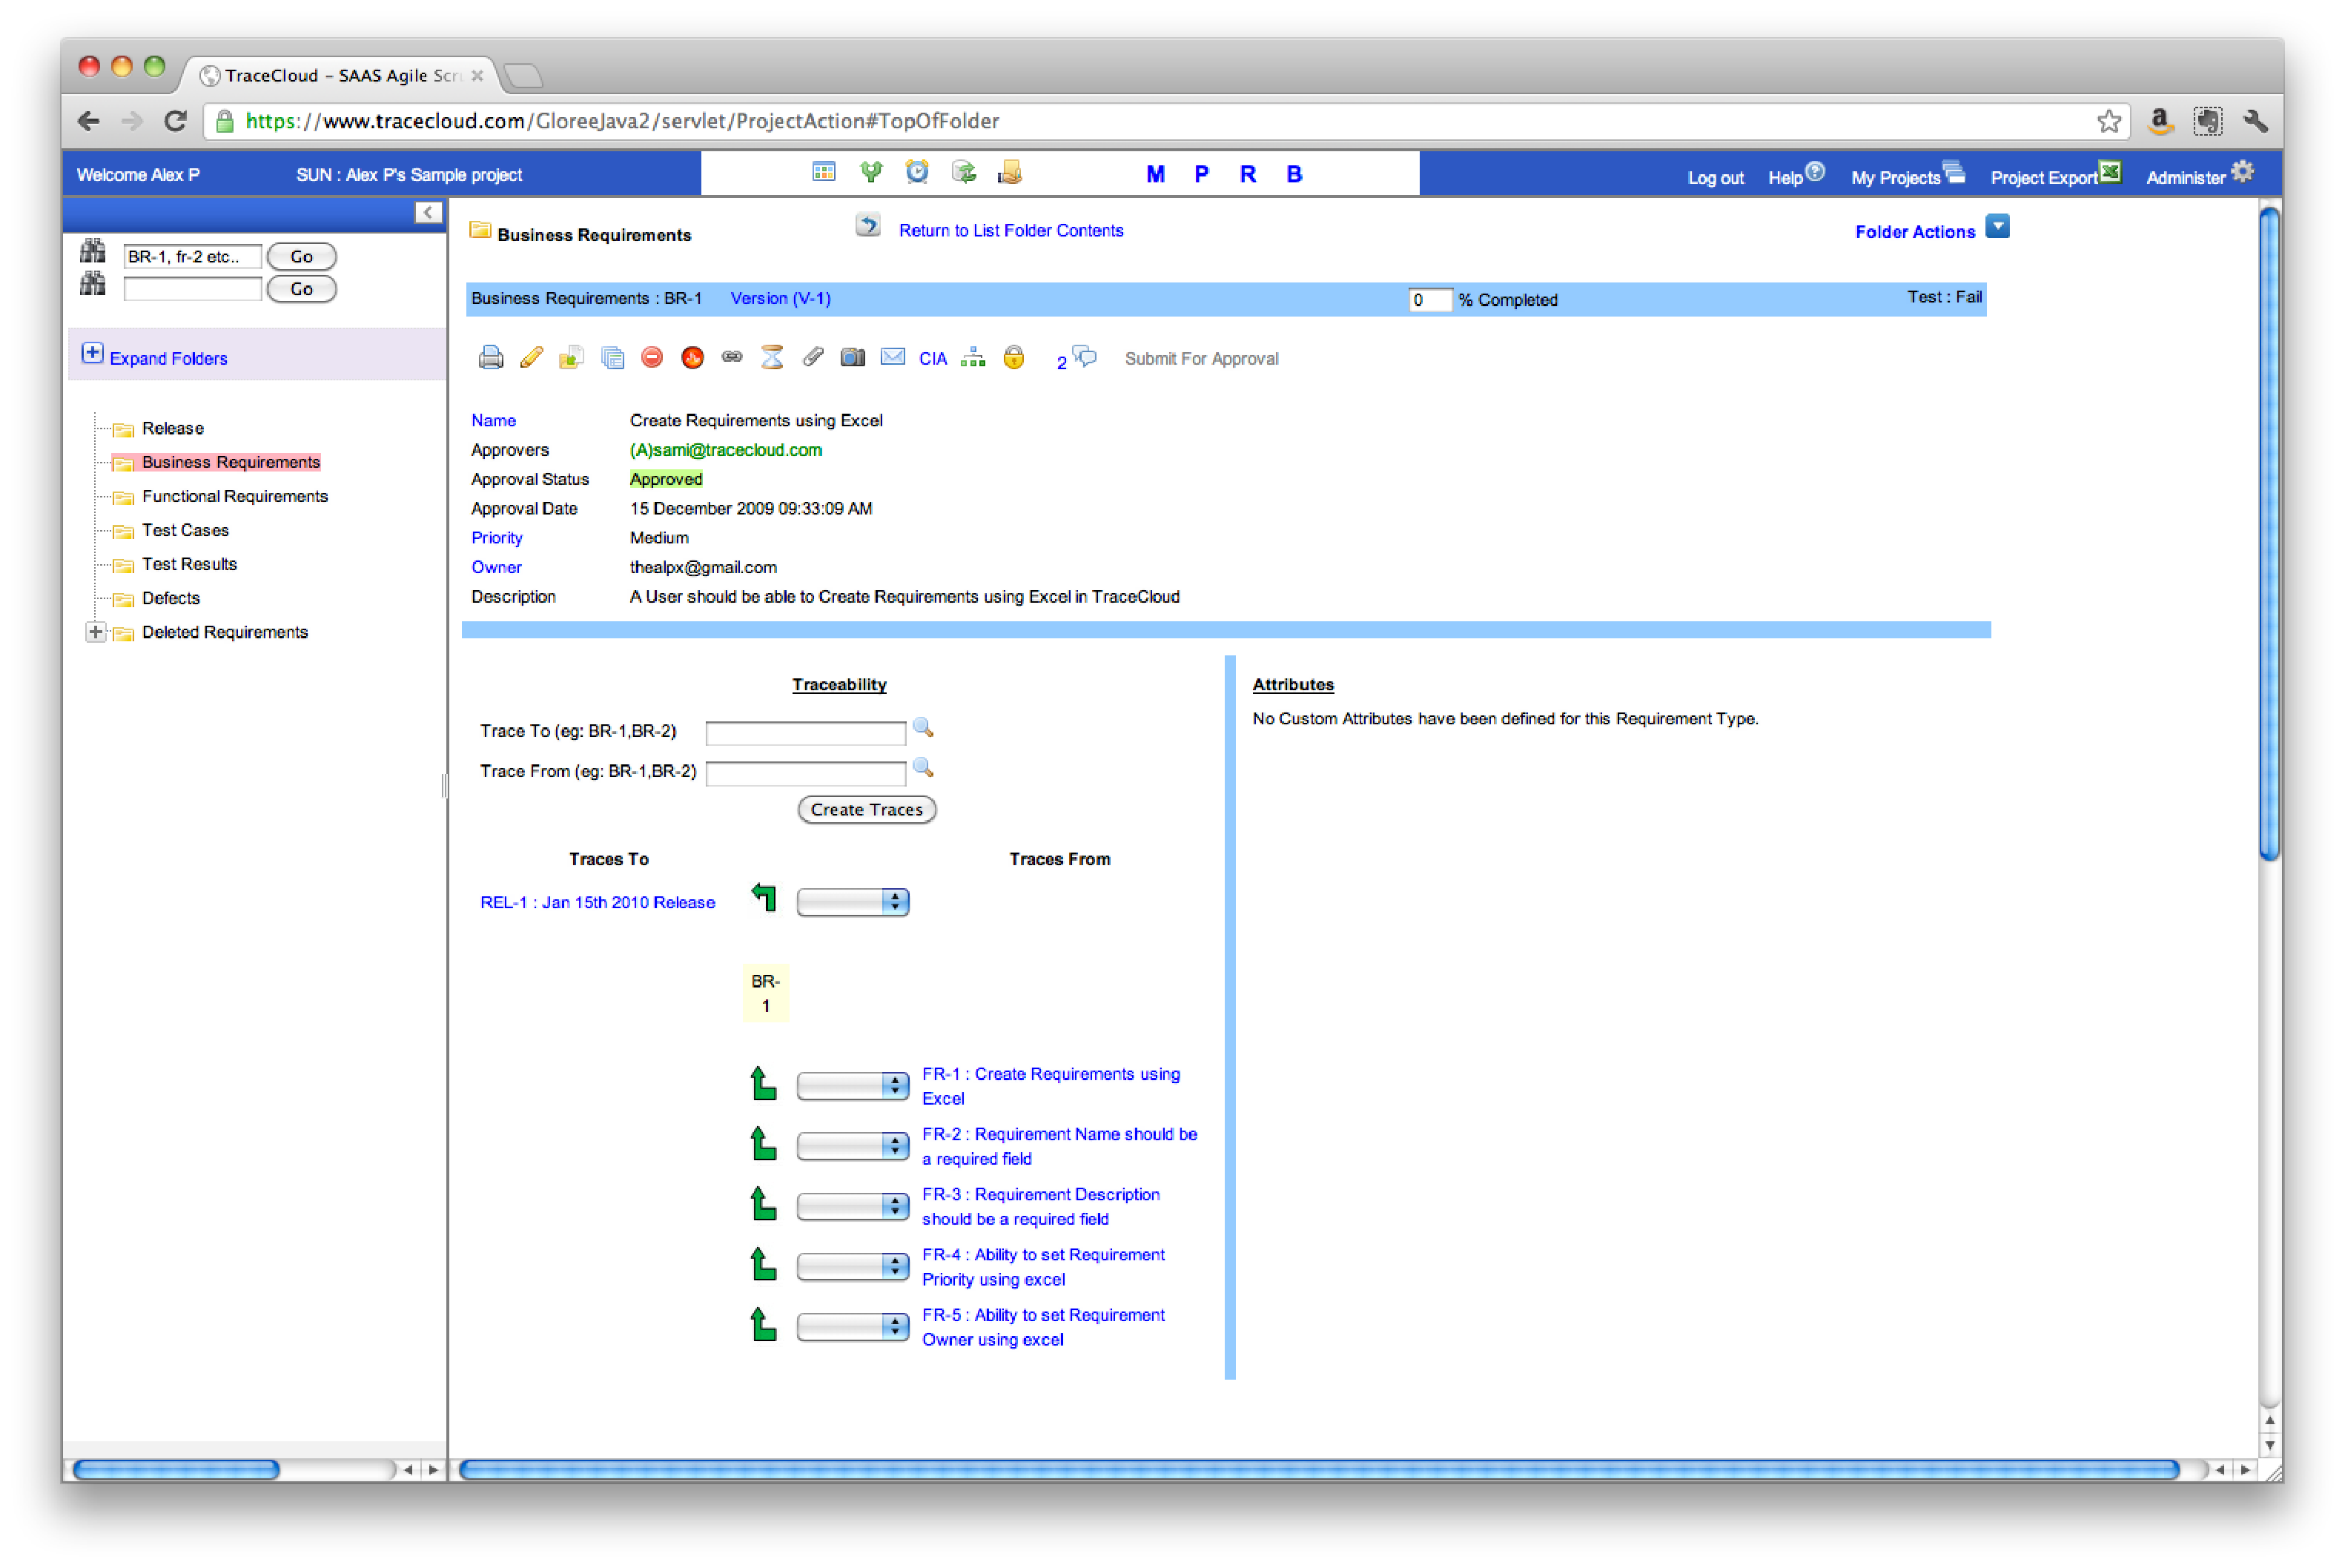
\includegraphics[width=1.0\textwidth]{img/tracecloud_4.pdf}
          \caption{Tracecloud - szczegóły wymagania}
          \label{fig:tracecloud_4}
        \end{figure*}

      \subsubsection{Tracecloud}
        
        Jak widać na rys. \ref{fig:tracecloud_1} Tracecloud jest znacznie gorzej przygotowany od strony interfejsu użytkownika. Mimo tego jest znacznie bardziej skompilkowanym systemem, udostępniającym znacznie więcej funkcjonalności niż Gatherspace.

        Główny przegląd projektu zawiera tabelę z wyświetlonymi metrykami projektu. Można z niej odczytać ilość zaimplementowanych wymagań, ilościowe wyniki testów, przedląd zgłoszonych błędów i wartości liczbowe wymagań pogrupowane w poszczególne statusy. Po dokładnym przeanalizowaniu tabeli, można odczytać interesujące informacje na temat projektu, jednak użyteczność tego sposobu reprezentacji stanu projektu jest bardzo niska. 

        Oprócz ilościowego przeglądu stanu projektu, użytkownik ma do dyspozycji menu i odnośniki do najważniejszych modułów systemu, taki jak wymagania biznesowe, funkcjonalne, scenariusze testowe i błędy.

        Przegląd wymagań opiera się o wykres ze statystykami oraz prostą listę (rys. \ref{fig:tracecloud_3}), z kolei szczegóły wymagania zawierają informację o jego nazwie, priorytecie, właścicielu oraz opis. Dodatkowo twórcy umieścili moduł śledzenia umożliwiający połączenie wymagań biznesowych z funkcjonalnymi (rys. \ref{fig:tracecloud_4}).
    
        Oprócz licznych raportów wyświetlanych w obrębie aplikacji, nie znaleziono funkcjonalności generowania dokmentu specyfikacji wymagań. 

        Tracecloud dostępny jest jako wersja Trial przez 6 miesięcy. Koszt wdrożenia waha się od 350\$ do 1000\$ za miesiąc użytkownania systemu w zależności od maksymalnej ilości obsługiwanych wymagań. Najtańsza licencja przewiduje obsługę do 5000 wymagań, podczas gdy wersja najdroższa - do 10tyś.

    \subsection{Aplikacje desktopowe}

      Model SaaS, mimo wszystkich swoich zalet, posiada również wady. Głównym powodem kontrowersji jest konieczność powierzenia danych biznesowych firmie udostępniającej narzędzie na swoich serwerach. Dla dużych korporacji, pilnie strzegących swoich tajemnic handlowych, takie rozwiązanie, może być nie do zaakceptowania ze względów bezpieczeństwa. Mimo potencjalnej możliwośći uniknięcia kosztów budowy i utrzymania infrastruktury sprzętowo-software'owej ryzyko związane z brakiem kontroli nad powierzonymi danymi jest często zbyt wielkie. 

      W klasycznych aplikacjach okienkowych, odpowiedzialność w zakresie zabezpieczenia danych spoczywa na samej korporacji i jej pracowniku. Dzięki temu, nadal istnieje zapotrzebowanie na oprogramowanie instalowane na lokalnym dysku użytkownika. Przykładami takich aplikacji są m.in. IBM DOORS oraz IBM Rational Requirements Composer.

      Rational Requirements Composer jest aplikacją zbudowaną przez firmę IBM. Dostępna jest wersja zbudowana na bazie platformy \emph{eclipse} jak również klient webowy, dostępny w przeglądarce internetowej na platformie IBM Jazz. Jest to potężne narzędzie wspierające kolaborację, śledzenie wymagań, audyty, raportowanie, graficzne modelowanie procesów biznesowych oraz zaawansowaną edycję dokumentów tekstowych. 

      Definiowanie wymagań w Rational Requriements Composer jest możliwe na wiele sposobów, m. in.: szablonowanie interfejsów, edycja tekstu, story boardy oraz przy użyciu wbudowanych w system kontrolek i szablonów.

      Przykładowy ekran definiowania wymagania umieszczono na Rysunku \ref{fig:rrc1}.

      \begin{figure*}[t]
        \centering
        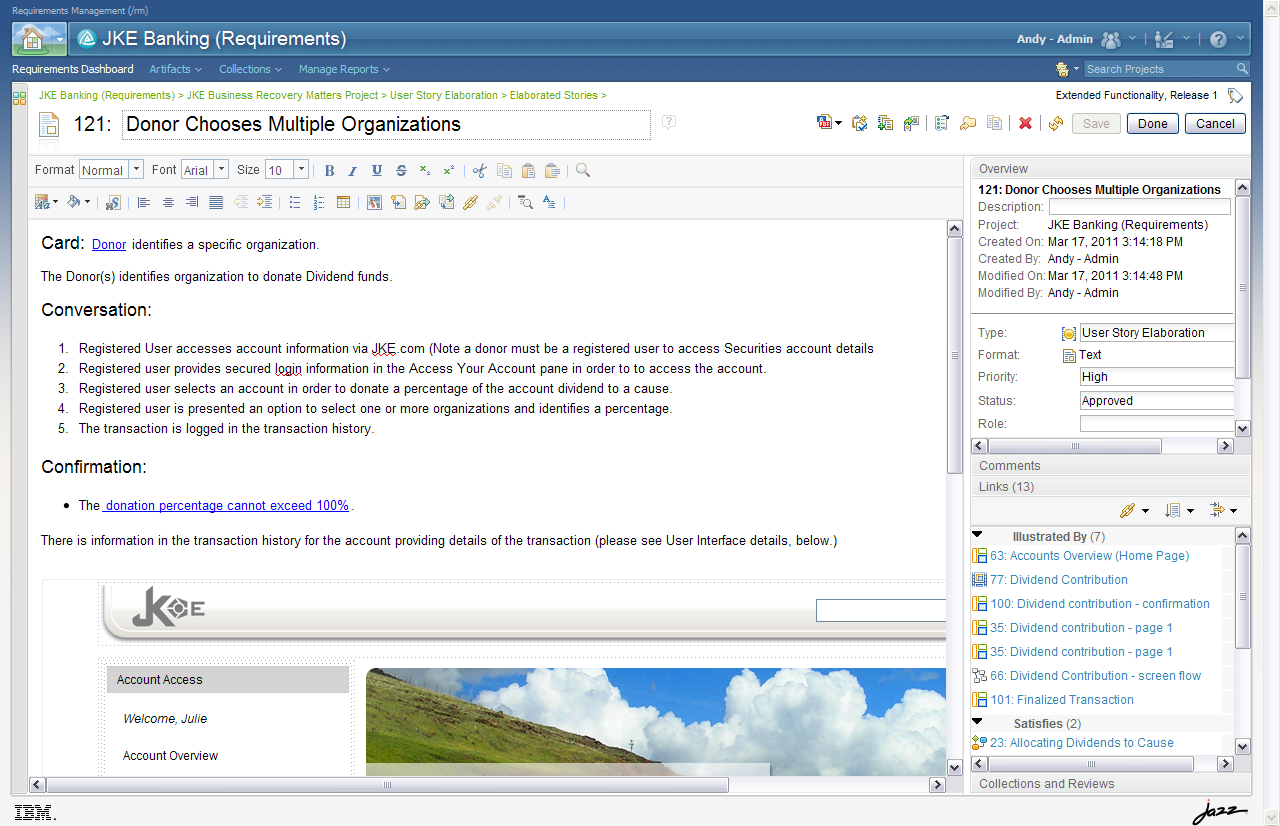
\includegraphics[width=1.0\textwidth]{img/rrc-primary.png}
        \caption{Rational Requisite PRO - definiowanie wymagania. Źródło: jazz.net}
        \label{fig:rrc1}
      \end{figure*}

      Platforma umożliwia również modelowanie procesów biznesowych w języku BPML (Business Process Modeling Language) (Rysunek \ref{fig:bpml}).

      \begin{figure*}[t]
        \centering
        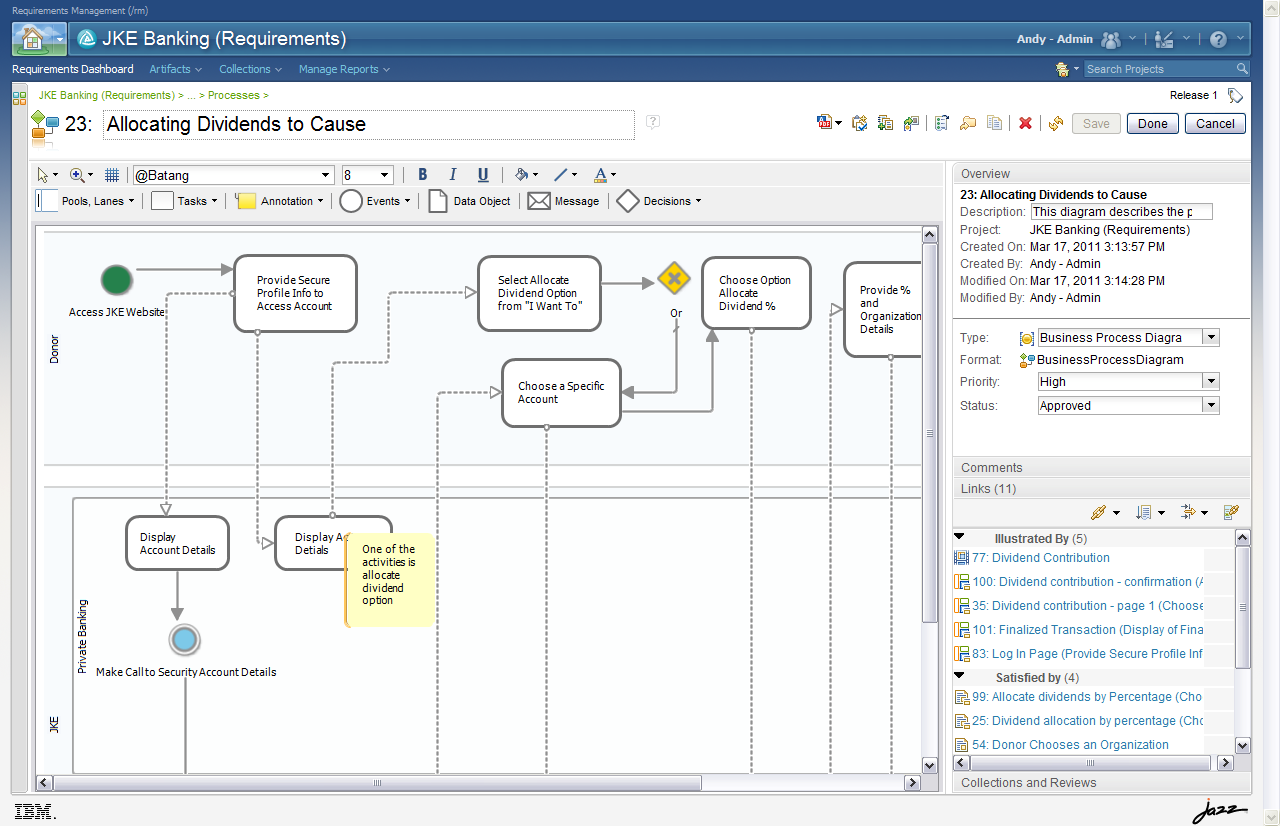
\includegraphics[width=1.0\textwidth]{img/visually-define.png}
        \caption{Rational Requisite PRO - definiowanie wymagania. Źródło: jazz.net.}
        \label{fig:bpml}
      \end{figure*}

      Zaawansowane narzędzia wspierające kolaborację, umożliwiają komunikację drogą elektroniczną, rewidowanie artefaktów, aktualizację statusów zadań i wiele innych (Rysunek \ref{fig:colla}). Z kolei audyty i historia zmian pozwalają na wspólne tworzenie i modyfikację dokumentów na zasadzie śledzenia podobną do tej znanej z pakietu MS Office (Rysunek \ref{fig:audit}).

      \begin{figure*}[t]
        \centering
        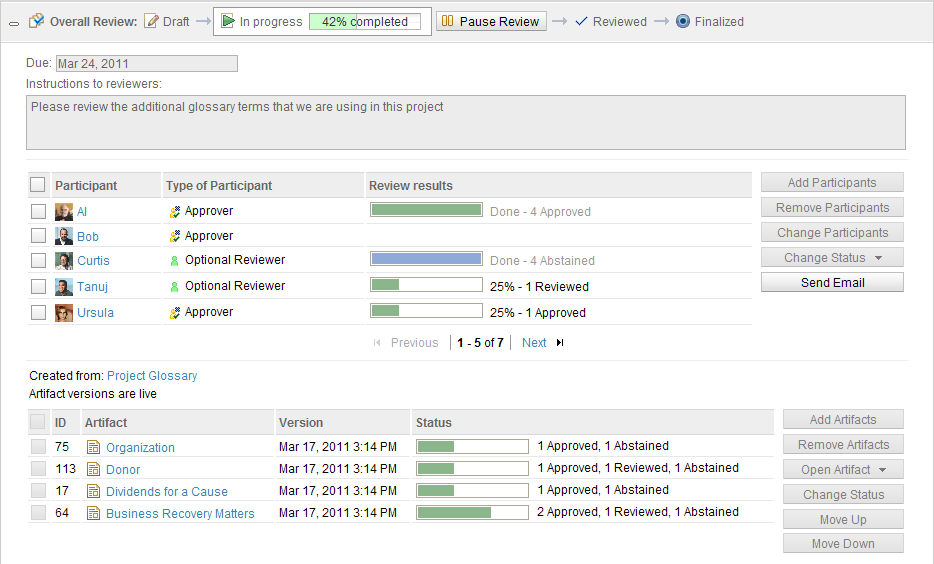
\includegraphics[width=1.0\textwidth]{img/review-and-collaboration.png}
        \caption{Rational Requisite PRO - kolaboracja. Źródło: jazz.net.}
        \label{fig:colla}
      \end{figure*}

      \begin{figure*}[t]
        \centering
        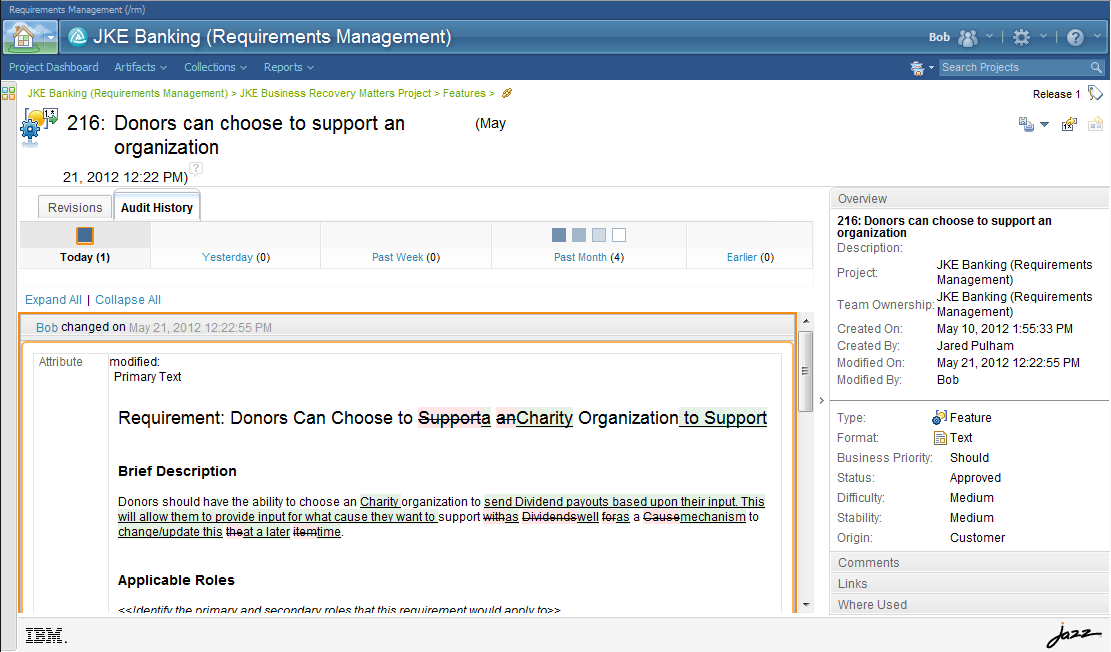
\includegraphics[width=1.0\textwidth]{img/audit-history.png}
        \caption{Rational Requisite PRO - historia zmian. Źródło: jazz.net.}
        \label{fig:audit}
      \end{figure*}

    \subsection{Platforma IBM .jazz}

      Platforma IBM Jazz zasługuje na osobną sekcję, ponieważ jest zintegrowanym, kompleksowym zestawem narzędzi i aplikacji dla przedsiębiorstw tworzących oprogramowanie. Centrum zarządzania platformą jazz jest serwer Jazz Team Server stanowiący repozytorium danych i ośrodek dowodzenia. Platforma składa się zarówno udostępnionych na serwerze usług sieciowych oraz aplikacji instalowanych lokalnie, łączących się ze zdalnym serwerem (tzw. rich-client applications). Ogólna architektura platformy została zaprezentowana na Rysunku \ref{fig:jts}. Interesującym rozwiązaniem w tym przypadku jest fakt, iż jazz.net stoni swojego rodzaju szynę integracyjną, pozwalającą na korzystanie z istniejącego oprogramowania zainstalowanego na licznych komputerach klienckich. Kompunikacja z aplikacjami klienckimi przebiega na bazie protokołu HTTP i webservice'ów RESTowych.

      \begin{figure*}[t]
        \centering
        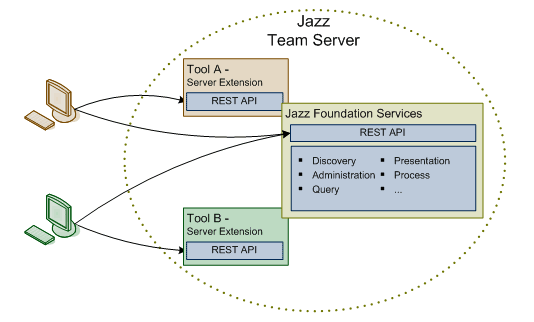
\includegraphics[width=1.0\textwidth]{img/jts.png}
        \caption{Platforma jazz.net - Jazz Team Server. Źródło: jazz.net}
        \label{fig:jts}
      \end{figure*}

  \section{Problemy z istniejącymi rozwiązaniami}

      Analizując istniejące rozwiązania, nie można oprzeć się wrażeniu, że wszystkie przystosowane są do dużych, korporacyjnych projektów. Większość aplikacji powiela rozwiązania znane i sprawdzone funkcjonalności. W konsekwencji trudnym zadaniem jest znalezienie wyróżniających się elementów wśród oferowanych możliwości tych produktów. Wyróżniają się szczególnie ciężkie aplikacje desktopowe od firmy IBM, jednak są one przystosowane do bardzo dużych projektów. Małe i średnie przedsiębiorstwa potrzebują prostszych i ,,lżejszych rozwiązań''. 

      Proces definiowania wymagań w niewielkich projektach jest w dużej mierze procesem twórczym. Często pojawienie się nowego wymagania jest inicjowane z kilku heterogenicznych źródeł. Nierzadko zdarza się również, że to samo wymaganie jest różnie komunikowane przez wiele źródeł. W niewielkich projektach, gdzie często jedna osoba, lub mały zespół odpowiedzialny jest za specyfikację wymagań, wymagania przybierają postać wiadomości email, rozmów telefonicznych, notatek ze spotkań i formalnych dokumentów. Zadaniem osoby lub zespołu odpowiedzialnego za specyfikację wymagań, jest przefiltrowanie cząstkowych informacji oraz ekstrakcja i udokumentowanie wymagań. Żadne narzędzie (przynajmniej na razie) nie zastąpi skutecznie pracy człowieka nad wyłuskaniem wszystkich wymagań. 

  \chapter{Podstawy teoretyczne i omówienie koncepcji proponowanego rozwiązania}
  
  W poprzednim rozdziale opisano przykładowe narzędzia funkcjonujące na rynku oprogramowania do zarządzania wymaganiami. Opisano ich główne wady i zalety oraz przedstawiono najważniejsze problemy związane ze stosowaniem ich w praktyce.

  W tym rozdziale, zostaną opisane procesy inżynierii wymagań od strony teoretycznej. Zostanie również zwrócona uwaga na niezbędne elementy nowoczesnego systemu wspierającego pracę z wymaganiami w małych i średnich przedsiębiorstwach. Na koniec rozdziału, przedstawiona zostanie koncepcja nowego narzędzia, będącego przedmiotem tej pracy.
  
  \section{Inżynieria wymagań}
    
    Inżynieria wymagań (IW) jest dziedziną, na którą składają się wszelkie działania związane z odkrywaniem (elicitation), analizą (analysis), weryfikacją (validation) oraz zarządzaniem wymaganiami \cite{Somm06}. Dotyczy ona każdego systemu informatycznego, niezależnie od jego rozmiarów i jest jednocześnie jednym z najistotniejszych procesów w cyklu życia projektu.

    IW dostarcza metodologii i narzędzi, służących do precyzyjnego określenia celu i zakresu projektu, poprzez identyfikację interesariuszy i ich potrzeb oraz udokumentowanie wyników w formie umożliwiającej ich analizę, komunikację oraz finalnie - implementację \cite{Nus00}. 

      \subsubsection{Zarys historyczny}

        Kryzys oprogramowania na przełomie lat '60 i '70 XX wieku był katalizatorem do podjęcia prób usystematyzowania młodej wówczas dziedziny tworzenia systemów informatycznych. Był to okres popularyzjacji sprzętu komputerowego, powszechnego, dramatycznie rosnącego zapotrzebowania na programistów oraz nagłośnionych, wielkich porażek systemów informatycznych, jak katastrofa rakiety kosmicznej Mariner 1 \cite{Brooks75}. Niedobór wykwalifikowanych programistów, zmusił korporacje do intensywnych poszukiwań nowych rozwiązań. Literatura branżowa szybko przepełniła się głosami nawołującymi do poprawy metod zarządzania w projektach informatycznych. Pojawiły się takie tytuły jak ‘‘Controlling Computer Programming’’, ; ‘‘New Power for Management’‘; ‘Managing the Programming Effort’’; ‘‘The Management of Computer Programming Efforts’’. W roku 1968, w drodze ustaleń na konferencji NATO Software Engineering (tu po raz pierwszy w branży zaczęto mówić o ,,kryzysie oprogramowania''), ''zarządzanie oprogramowaniem'' stało się fundamentem i jednym z głównych dyskursów w dziedzinie inżynierii oprogramowania \cite{Ense03}.
        
        Pionierzy inżynierii oprogramowania podejmowali próby zaczerpnięcia wiedzy z zakresu inżynierii systemów i wykorzystania jej w projektach informatycznych. Ten kierunek rozwoju opierał się na paradygmacie klasycznej inżynierii, zakładającym budowę systemu zgodną z określonym procesem: od identyfikacji problemu, opracowaniu specyfikacji, konstrukcji systemu i jego utrzymania. Takie sekwencyjne podejście do tworzenia systemów informatycznych było fundamentem powstania pierwszych procesów wytwórczych oprogramowania. 
        
        Klasycznym podejściem był przedstawiony w pracy Winstona Royce'a (1970), model kaskadowy (sekwencyjny model liniowy)\footnotemark. \footnotetext{Royce podał w swoim modelu wariant liniowego procesu, gdzie kolejne fazy były zwrotnie sprzężone z fazami poprzednimi \cite{RWins70}, jednak w większości organizacji stosujących model kaskadowy, jest to ściśle sekwencyjny proces liniowy \cite{pressman2010software}.} W swojej pracy, Royce proponując rozwiązanie sekwencyjne (w którym żaden kolejny etap nie mógł zostać rozpoczęty przed zakończeniem etapu poprzedniego) zastrzegł, że ,,wierzy w zaproponowaną koncepcję, jednak jej implementacja jest ryzykowna i naraża projekty na niepowodzenie'' \cite{RWins70}. Zatem już na samym początku swojego istnienia, model kaskadowy wraz z analogią inżynierii oprogramowania do inżynierii klasycznej, był uważany w branży za nieprzystosowany do dziedziny problemu. Mimo tego, model kaskadowy, z powodzeniem, znalazł zastosowanie w dużych projektach m. in. rządowych, wojskowych i kosmicznych, gdzie zarówno klient jak i wykonawcy bardzo dobrze rozumieli wymagania systemu \cite{NasaSE}. W kolejnych latach pojawiały się modyfikacje modelu kaskadowego, a rola podejścia iteracyjnego przybierała na znaczeniu. W roku 1986 Barry Boehm opisał model spiralny, będący połączeniem ustrukturalizowanego procesu kaskadowego z rozwojem przyrostowym, opartym na prototypowaniu \cite{Boehm86}. Kolejnym kamieniem milowym w dziedzinie procesów wytwórczych oprogramowania było wydanie książki Kent'a Beck'a ,,Extreme Programming Explained'' \cite{KBeck00} w roku 1999 oraz publikacja ,,Agile Manifesto'' w roku 2001, gdzie po raz pierwszy, formalnie zaproponowano termin ,,zwinnego programowania'' \cite{MFowl01}. 
      
      \subsubsection{Podobieństwa w procesach wytwórczych}

        Pomimo znaczących różnic w dostępnych i udokumentowanych metodykach projektowych, dla wszystkich istnieje część wspólna, w postaci nieuniknionej fazy analizy na etapie rozpoczęcia projektu. Nie ma możliwości rozpoczęcia modelowania ani implementacji systemu, bez wcześniejszej wiedzy w zakresie jego przeznaczenia i oczekiwanych funkcji. Zarówno w metodykach zwinnych, jak i w tradycyjnych procesach wytwórczych, w początkowej fazie projektu, kluczową rolę gra przygotowanie systemu od strony wymagań. Zatem inżynieria wymagań dotyczy każdego procesu wytwórczego.

      \subsubsection{Procesy w inżynierii wymagań}

      Jak podaje Sommerville \cite{Somm06}, do dziedziny inżynierii wymagań możemy zaliczyć następujące pod-procesy:

      \begin{itemize} 
          \item studium wykonalności 
          \item gromadzenie i analiza wymagań
          \item weryfikacja wymagań
          \item zarządzanie wymaganiami
      \end{itemize}

      \subsubsection{Studium wykonalności (feasibility study)}

        Wg. Sommerville'a (2006), przy dużych projektach, w początkowym stadium powinno zostać przeprowadzone studium wykonalności. Podstawowym celem jego przeprowadzania jest udzielenie odpowiedzi na pytanie, czy należy kontynuować projekt. W trakcie tego etapu zwiększa się wiedza o dziedzinie problemu, a koncepcja systemu jest weryfikowana pod kątem celowości zastosowania w organizacji, wszelkich ograniczeń systemowych, a także sprzętowych. W modelu Rational Unified Process, studium wykonalności powinno zostać włączone do fazy rozpoczęcia projektu (inception phase) \cite{Kruch03}.

        W niektórych przypadkach (szczególnie w dużych projektach krytycznych) studium wykonalności może zostać rozbudowane do pełnej analizy oceny ryzyka. Wówczas powinny zostać uwzględnione aspekty nietechniczne i administracyjne, np.: czy projekt ma przydzielony wystarczający budżet, jakie aspekty polityczne należy wziąć pod uwagę w trakcie definiowania wymagań, czy projekt może być wykonany w przyjętych ramach czasowych.

      \subsubsection{Gromadzenie i analiza wymagań}

        Gromadzenie wymagań jest procesem, na który składają się działania zmierzające do zgłębienia celu i motywacji przyświecających budowie analizowanego systemu. W szczególności etap ten wiąże się z identyfikacją wszystkich wymagań, jakie musi spełnić system, aby osiągnąć sukces.
        
        Proces gromadzenia wymagań w języku angielskim nosi nazwę ,,requirements elicitaion''. ,,Elicitaion'' w dosłownym tlumaczeniu, oznacza ,,wywołanie'', ,,wydobycie'', ,,ujawnienie''. W szczególności termin ,,wydobycie'' lepiej oddaje naturę tych działań, niż popularne w języku polskim ,,gromadzenie'' czy ,,definiowanie'' wymagań. Innymi słowy jest to proces komunikacji analityków z użytkownikami w celu zdobycia jak największej ilości informacji o budowanym systemie. 

        Głównymi technikami związanymi z pozyskiwaniem wymagań są: identyfikacja interesariuszy, gromadzenie faktów i informacji przy pomocy wywiadów, kwestionariuszy, list kontrolnych, warsztatów kreatywnych, burzy mózgów, map myśli (mindmapping), modelowania i prototypowania. Znaczna część wymagań stanowi wiedzę zdobytą w procesie przeprowadzania wywiadów z interesariuszami projektu. W związku w powyższym, można wprowadzić uniwersalne uogólnienie, stwierdzając, że głównym narzędziem wykorzystywanym w procesie gromadzenia wymagań jest szeroko rozumiana komunikacja. Wywiady przeprowadzane z interesariuszami mogą mieć formalny lub nieformalny przebieg, a stosowane w tym procesie narzędzia w dużej mierze zależą od poziomu skomplikowania projektu, wypracowanych metod, dostępnych narzędzi i preferencji samych analityków. 
        
        Wymagania zwykle pochodzą z wielu heterogenicznych źródeł. Najwyższy priorytet zawsze powinien przysługiwać wymaganiom pochodzącym od klienta i użytkowników systemu. Jednak wpływ na specyfikację systemu mogą mieć również źródła zewnętrzne, takie jak niezależni eksperci z dziedzin obejmowanych przez projekt, uwarunkowania prawne i ekonomiczne, czy ogólnie przyjęte standardy i procedury związane ze szczególnymi aspektami tworzonego systemu.

        Dokumentem stanowiącym rezultat pracy nad gromadzeniem wymagań jest specyfikacja wymagań systemu. Standardem określającym proces tworzenia i strukturę tego dokumentu jest IEEE Guide for Developing System Requirements Specifications \cite{institute1984ieee}. Wiele organizacji definiuje również własne standardy i procesy, lepiej odpowiadające specyfice realizowanych projektów.

        Do procesu gromadzenia wymagań i narzędzi z nim związanych, autor powróci przy okazji opisu koncepcji proponowanego rozwiązania, w następnym rozdziale.

      \subsubsection{Weryfikacja wymagań}

        Celem procesu weryfikacji wymagań jest dowiedzenie, że koncepcja budowanego systemu odpowiada rzeczywistym potrzebom użytkowników. Jest to kluczowy proces inżynierii wymagań, ponieważ poprawa zidentyfikowanych na tym etapie problemów jest o rząd wielkości mniej kosztowna, niż późniejsze zmiany systemowe. Zdecydowanie łatwiej jest bowiem poprawiać projekt architektury opgrogramowania niż wprowadzać modyfikacje koncepcyjne w istniejącym już systemie. 

        Weryfikacja wymagań powinna być przeprowadzana na podstawie dokumentu specyfikacji wymagań systemu. Działania podejmowane w trakcie weryfikacji wymagań powinny uwzględniać przede wszystkim zasadność, bezkonfliktowość, kompletność, implementowalność i weryfikowalność wszystkich wymagań. Zasadność pozwala odpowiedzieć na pytanie, czy dane wymaganie rozwiązuje realny problem w systemie, potwierdzając tym samym celowość swojego istnienia. Ponieważ w trakcie gromadzenia wymagań przeprowadzane są wywiady z wieloma interesariuszami projektu, mającymi różne, często sprzeczne wymagania, konieczna jest weryfikacja spójności specyfikacji pod względem konfliktów. Zapewnienie bezkonfliktowości polega na takim sfomułowaniu wymagań w specyfikacji, aby żadne nie były ze sobą w sprzeczności. Kompletność jest weryfikacją dokumentu wymagań z perspektywy realizacji wszystkich porządanych funkcji. Wszystkie zdefiniowane wymagania muszą być realizowalne w określonym czasie, przy użyciu określonego sprzętu i opgrogramowania. W trakcie badania implementowalności, analityk skupia się na odpowiedzi na pytanie czy dane wymaganie jest w pełni realizowalne w rzeczywistych warunkach. Z kolei weryfikowalność ma na celu zapewnienie narzędzi, umożliwiających sprawdzenie i demonstrację poprawności działania zrealizowanego wymagania za pomocą metod empirycznych.

        Istnieje wiele narzędzi i metod, jakie można wykorzystać w procesie weryfikacji wymagań. Wyniki badania Boehem et al ,,Prototyping vs. Specifying'' \cite{Boehm84} dowodzą, że jedną ze skuteczniejszych metod prewencji przed definiowaniem błędnych wymagań jest metoda prototypowania. Badanie to polegało na podziale grupy studentów inżynierii oprogramowania na dwa zespoły. Celem obu zespołów była implementacja systemu o określonym zakresie. Jedna grupa korzystała z metody prototypowania. Ich konkurenci, natomiast, korzystali z podejścia zorientowanego na specyfikację. W rezultacie, grupa stosująca metodę prototypowania osiągnęła lepsze wyniki, w szczególności, w zakresie użyteczności interfejsu użytkownika i prostoty obsługi dostarczonego systemu. W przeciwieństwie do podejścia opartego na samej specyfikacji, prototypowanie umożliwia wizualizację wymagań systemu, uniezależniając interpretację treści wymagania od wyobraźni odbiorcy. 

        Jednak, jak każda metoda, prototypowanie nie jest wolne od wad. Istnieje ryzyko, że prototyp, kładąc zbyt duży nacisk na pewne szczegóły, sprawi, że ogólna koncepcja systemu przestanie być wyraźnie dostrzegalna. Ponadto, wyzwaniem w przypadku prototypowania jest odpowiednia komunikacja z klientem. Klient musi dokładnie rozumieć specyfikę i cel tworzenia prototypu. Istnieje bowiem pokusa, aby pod naciskami klienta wykorzystać prototyp jako finalny produkt. W związku z powyższym, wśród wszystkich członków zespołu, niezbędna jest pełna świadomość faktu, iż prototyp, po spełnieniu swojej funkcji zostanie odstawiony, a doświadczenia z jego budowy posłużą jako informacje wejściowe do implementacji finalnego rozwiązania. Powstało wiele prac dotyczących prototypowania, jednak szczegółowe aspekty tego podejścia wykraczają poza zakres tej pracy. Osoby zainteresowane metodami prototypowania znajdą kilka ciekawych pozycji w bibliografii \cite{arnowitz2006effective, budde1992prototyping}.

      \subsubsection{Zarządzanie wymaganiami}

        Specyfika większości projektów informatycznych, wiąże się z tym, że raz udokumentowane wymagania rzadko pozostają aktualne do momentu zakończenia prac. Wymagania są przedmiotem ciągłych zmian i niezbędne są narzędzia, których zadaniem będzie zarządzanie tymi zmianami. Proces zarządzania wymaganiami należy rozpocząć w momencie powstania pierwszej wersji specyfikacji wymagań i kontynuować aż do zakończenia projektu.

  \section{Motywacja}

    Mając na uwadze teoretyczne tło dziedziny jaką jest inżynieria wymagań oraz praktyczne problemy z jakimi borykają się dzisiaj małe i średnie przedsiębiorstwa w zakresie zarządzania wymaganiami, powstała koncepcja rozwiązania, adresującego najpilniejsze problemy w rzeczywistych projektach małej i średniej skali. 

    Jak wykazano w rozdziale 2, pomimo rozwoju technologii oraz świadomości firm w zakresie inżynierii oprogramowania, bardzo duża część małych \linebreak i średnich przedsiębiorstw nadal ignoruje zagadnienia z zakresu inżynierii wymagań. Dojrzałość tych organizacji pod kątem inżynierii oprogramowania jest bardzo niska. Niewielką część harmonogramów projektów przeznacza się na analizę wymagań, a narzędzia stosowane w trakcie tego procesu najczęściej ograniczają się do pakietów biurowych, klientów poczty elektronicznej i odręcznych notatek. Mikro-firmy osiągająjące na tym polu sukcesy najczęściej charakteryzują się posiadaniem bardzo małych zespołów ekspertów z ogromym doświadczeniem w branży, posiadającymi techniki wypracowane metodami prób i błędów, nad którymi pracowali przez wiele lat w swojej karierze.  Jednak zdecydowana większość firm nadal eksperymentuje z autorskimi podejściami, często integrując różne istniejące narzędzia. 
    
    Część winy za taki stan rzeczy leży po stronie twórców oprogramowania. Istnieje niewiele systemów umożliwiających skuteczne zarządzanie wymaganiami w środowsiku dynamicznych, zorientowanych na rynek internetowy, projektów, jakie najczęściej realizują firmy z sektora MŚP. Kolejną ważną obserwacją jest fakt, iż bardzo często mamy do czynienia z projektami, których wymagania wymyślane są przez samych twórców, przez co proces dokumentowania wymagań i tworzenia specyfikacji przebiega ad hoc lub nie istnieje w ogóle. Dodatkowo, brak umiejętności zarządzania zmianą, powoduje, że projekty oddawane są po terminie, z przekroczonym budżetem, często niedostarczając klientowi porządanego efektu. Jest to problem całej branży - zarówno kadry zarządzającej, analityków, programistów, klientów i użytkowników. Problemy z zarządzaniem wymaganiami, powodują, spowolnienie innowacji. Gdyby firmy zaczęły umiejętnie zarządzać wymaganiami i zmianą, więcej projektów kończyłoby się sukcesem, co pozytywnie wpłynęłoby na prędkość rozwoju oprogramowania. Ewidentnie istnieje niezagospodarowana luka na rynku w tym segmencie. 

    Małe i średnie przedsiębiorstwa są motorem napędowym dzisiejszej gospodarki opartej w znacznym stopniu o techniki informacyjne. Obowiązkiem inżynierii oprogramowania jest stałe kwestionowanie istniejących rozwiązań i katalizowanie zmian w kierunku usprawniania procesów związanych z wytwarzaniem oprogramowania. Jednak inżynieria wymagań zdaje się być niedocenianym i nadal słabo rozumianym zagadanieniem związanym z wytwarzaniem oprogramowania. Jest to jednak kluczowa, przyszłościowa dziedzina - w miarę postępu technologicznego, zapotrzebowanie na oprogramowanie nadal będzie wzrastało.

  \section{Opis proponowanego rozwiązania}

    Proces pozyskiwania i przetwarzania wymagań powinien być przede wszystkim łatwy w implementacji dla organizacji oraz dający dużą dozę elastyczności. W rozdziale 'Problemy z istniejącymi rozwiązaniami' opisano stan sztuki i zaadresowano niedociągnięcia dzisiejszych narzędzi. 

    Motywem przewodnim proponowanego narzędzia jest przystępność i prostota obsługi oraz wniesienie rzeczywistej wartości dodanej poprzez dostarczenie funkcji, mających realne zastosowanie w praktyce. 

    W trakcie prac nad koncepcją narzędzia postawiono następujące cele:
    
    \begin{itemize}
      \item Silna koncentracja na praktycznym zastosowaniu systemu wsparcia zarządzania wymaganiami - system musi rozwiązywać rzeczywiste problemy zespołów projektowych w zakresie gromadzenia i przetwarzania wymagań. Wdrożenie systemu musi wiązać się z wniesieniem wartości dodanej do procesów inżynierii wymagań w organizacji;
      \item Obsługa wielu projektów w obrębie aplikacji - system musi umożliwiać obsługę i zarządzanie wieloma projekami w obrębie tej samej aplikacji;
      \item Ogólny przegląd stanu projektu - najistotniejsze informacje z perspektywy wymagań systemu powinny być dostępne na jednej stronie podsumowującej projekt;
      \item Wsparcie gromadzenia wymagań - system powinien wspierać pozyskiwanie, definiowanie, katalogowanie (grupowanie) nieprzetworzonych wymagań oraz nadawanie im odpowiednich priorytetów przy pomocy intuicyjnych narzędzi;
      \item Uniwersalność formatu przechowywanych danych - system powinien umożliwiać łatwe przetwarzanie treści wymagań przez zewnętrzne systemy;
      \item Dostarczenie rozwiązań zarządzania zmianą - aplikacja powinna dostarczać wsparcia zarządzania wymaganiami na późniejszych etapach projektu;
      \item Stworzenie centralnego repozytorium wiedzy na temat wymagań - system powinien stanowić główne źródło wiedzy i komunikacji w zakresie wymagań;
      \item Wsparcie kolaboracji - system powinien umożliwiać współpracę nad wymaganiami poprzez obsługę wielu użytkowników i dostarczenie im modułu komentarzy;
      \item Automatyzacja tworzenia specyfikacji - należy zaimplementować algorytm generujący dokument specyfikacji wymagań na podstawie informacji dostępnych w systemie;
    \end{itemize}

    W efekcie powstał prototyp systemu, otwierający drogę do dyskusji i rozwoju w kierunku poprawienia procesów inżynierii wymagań w małych i średnich przedsiębiorstwach, skupiający się na praktycznych rozwiązaniach. 

  \section{System Reqmanager - opis funkcjonalności}

    Poniżej opisano poszczególne funkcjonalności systemu i przedstawiono mechanizmy, narzędzia oraz techniczne rowiązania które posłużyły do implementacji poszczególnych założeń systemu.

    \subsection{Obsługa wielu projektów} 
      System umożliwia tworzenie wielu projektów. Formularz dodawania projektu składa się pól nazwy, krótkiego opisu oraz głównej notatki projektu, będącej jego szczegółowym opisem w formie tzw. briefu. Ostatnią niezbędną informacją, którą należy podać jest planowana data zakończenia prac nad projektem. W założeniu opis i notatka projektu ulegają zmianom w miarę upływu czasu, dlatego na późniejszych etapach projetku istnieje możliwość bardzo łatwej edycji zmian treści tych atrybutów. 

    \subsection{Ogólny przegląd stanu projektu}
      Ekranem głównym w obrębie wybranego projektu jest przegląd stanu projektu z perspektywy wymagań. Użytkownik ma możliwość natychmiastowej edycji głównej notatki opsiującej założenia całego projektu oraz jego krótki opis. Ponadto, dostępna jest lista wymagań zawierająca podstawowe informacje takie jak kod wymagania, jego opis, priorytet oraz ilość przypisanych przypadków użycia. Wszystkie te elementy umieszczone na jednej stronie, umożliwiają użytkownikowi ogólną orientację w zakresie i celach projektu pod kątem wymagań. 

    \subsection{Wsparcie gromadzenia wymagań}
      Praktyczne narzędzie do zastosowania w procesie gromadzenia wymagań musi wspierać najwcześniejszą fazę - powstawania wymagań. W dynamicznych projektach, wymagania pojawiają się niespodziewanie, w różych sytuacjach i pochodzą z wielu różnych źródeł. Narzędzie musi wspierać prostą w obsłudze opcję dodawania wymagań w postaci krótkich notek, dłuższych artykułów lub opisów całych procesów. Jednocześnie nie może obarczać użytkownika obowiązkiem nadawania identyfikatorów oraz innych meta-informacji. Powinno również ograniczać potrzebę formatowania treści. Celem użytkownika, jest spisanie jak najszybciej wszystkich obserwacji i zachowanie ich w formie możliwej do późniejszego przetworzenia.

      Proponowane rozwiązanie wspiera ten proces dzięki zintegrowanemu edytorowi tekstu, edytorowi diagramów przypadków użycia oraz systemowi załączników.
      

      \subsubsection{Edytor tekstowy}

      Formatowanie tekstu w języku znaczników Markdown \cite{Grub04} umożliwia nadanie dokumentowi logicznej struktury wykorzystując zwykły tekst (plain text) zaopatrzony w odpowiednie oznaczenia. Dzięki temu użytkownik otrzymuje czytelny dokument, przy jednoczesnym ograniczeniu formy graficznej, która jest w tym konekście drugoplanowa. Przykład składni dokumentu Markdown zaprezentowano na listingu \ref{lst:markdownStx}.

      \begin{lstlisting}[caption={przykład składni języka Markdown}, label={lst:markdownStx}]
        # Brief projektu

        Ten dokument zawiera tzw "brief" projektu - wstepny opis 
        systemu, jaki mamy zamiar zbudowac.

        ## System w musi uwzgledniac 
        nastepujace funkcjonalnosci:
       
        * logowanie uzytkownika
        * dodawanie i zarzadzanie projektami
        * dodawanie i zarzadzanie wymaganiami
        * _tworzenie diagramow przypadkow uzycia_
      \end{lstlisting}
      
      Po konwersji przez Markdown do języka HTML, otrzymamy następujący wynik:

      \begin{lstlisting}[caption={wynik konwersji powyższego kodu do HTML}, label={lst:markDownCompile}]
        <h1>Brief projektu</h1>

        <p>Ten dokument zawiera tzw "brief" projektu - wstepny opis systemu, jaki mamy zamiar zbudowac.</p>

        <h2>System musi uwzgledniac nastepujace funkcjonalnosci:</h2>

        <ul>
          <li>logowanie uzytkownika</li>
          <li>dodawanie i zarzadzanie projektami</li>
          <li>dodawanie i zarzadzanie wymaganiami</li>
          <li><em>tworzenie diagramow przypadkow uzycia</em></li>
        </ul>
      \end{lstlisting}
  
      Dzięki temu, w łatwy sposób istnieje możliwość tworzenia spójnych dokumentów o logicznej strukturze, przy niewielkim nakładzie pracy.

      \subsubsection{Edytor diagramów UML}

      Edytor diagramów UML umożliwia wzbogacenie treści wymagania o graficzną reprezentację powiązanych przypadków użycia. Moduł ten wspiera współdzielenie diagramów pomiędzy wieloma wymaganiami, umożliwiając oznaczanie odpowiednich elementów jako odpowiedzialnych za realizację aktualnie opracowywanego wymagania. 

      Szczególnie istotnym elementem systemu jest generowanie obiektów aplikacji na podstawie danych odczytywanych bezpośrednio ze struktury diagramu. W efekcie, po utworzeniu elementu na diagramie i odpowiednim powiązaniu go z danym wymaganiem, powstanie reprezentacja tego elementu w postaci obiektu klasy Groovy, który następnie zostanie zapisany do bazy danych dzięki mapowaniu obiektowo - relacyjnemu będącego integralną częścią frameworka Grails. Jednocześnie zostanie zachowana odpowiednia relacja między utworzonym obiektem klasy UseCase, a wymaganiem. Mapowanie elementów utworzonych na diagramie przebiega dzięki możliwości serializacji diagramu do formatu XML. Szczegółowo autor opisuje ten mechanizm w rozdziale dotyczącym rozwiązań implementacyjnych.

      W przyszłości, istnieje możliwość rozszerzenia funkcjonalności edytora o kolejne rodzaje diagramów UML. Ponadto, w trakcie ewentualnej rozbudowy systemu, wygodnym usprawnieniem byłoby automatyczne przypisywanie nowo utworzonych obiektów do aktualnie edytowanego wymagania.

      \subsubsection{System załączników}

      System załączników dodatkowo wzbogaca możliwości ekspresji - do wymagania użytkownik może dodać dokumenty lub treści multimedialne powiązane z danym wymaganiem, mające na clu lepsze zrozumienie istoty problemu.

    \subsection{Uniwersalność formatu danych}
      Narzędzie do zarządzania wymaganiami powinno ułatwiać późniejsze procesowanie wprowadzonych do niego danych. Proponowany system realizuje tę potrzebę przechowując wszystkie wymagania oraz powiązane diagramy w bazie danych. Treść opisu wymagań jest przechowywana w postaci zwykłego tekstu, zaopatrzonego w znaczniki Markdown. Dzięki temu, treść wymagań jest znacznie łatwiejsza w przetwarzaniu, niż dokumenty tworzone przez klasyczne edytory tekstu.
      
      Struktura diagramów powiązanych z wymaganiami jest przechowywana w bazie danych w formacie xml. Takie podejście również w znacznym stopniu ułatwia późniejsze przetwarzanie informacji zawartych na diagramach. 
      
      System aktywnie wykorzystuje powyższe właściwości podczas automatycznego generowania specyfikacji wymagań.

    \subsection{Zarządzanie zmianą}
      Zarządzanie zmianą jest istotne z punktu widzenia ewolucji wymagań i stopniowego uszczegóławiania dokumentacji systemu. Proponowane narzędzie wspiera ten proces zachowując poprzedni stan wymagania w trakcie jego zapisu. Dzięki temu możliwe jest prześledzenie zmian dokonywanych w wymaganiach. 

    \subsection{Centralne repozytorium}
      Proponowany system jest dostępny przez przeglądarkę, dzięki czemu stanowi centralne repozytorium wiedzy na temat wymagań w projekcie. Interfejs www z elementami html5 powoduje, że narzędzie wymaga jedynie nowoczesnej przeglądarki internetowej, bez żadnych dodatkowych wtyczek. Dzięki temu aplikacja cechuje się wysokim poziomem dostępności.  

    \subsection{Kolaboracja}
      Możliwość komentowania wymagań została zaimplementowana z myślą o umożliwieniu kolaboracji nad wymaganiami członkom zespołu.

    \subsection{Generator specyfikacji}
      Jedną z kluczowych funkcjonalności proponowanego rozwiązania jest automatyczne generowanie dokumentu specyfikacji wymagań na podstawie aktualnych danych w systemie.
      Użytkownik w każdej chwili jest w stanie wygenerować bieżącą wersję specyfikacji i poddać ją całościowej analizie. Częścią specyfikacji zostają zarówno wymagania jak i powiązane z nimi przypadki użycia.

    \subsection{Praktyczne zastosowanie}
      Proponowane funkcjonalności są oparte na rzeczywistych doświadczeniach, w rzeczywistych projektach w małych i średnich przedsiębiorstwach. Bazują na silnym przekonaniu, że narzędzie, aby było wykorzystywnane, musi być wygodne i proste w użyciu oraz wnosić wartość dodaną do istniejącej infrastruktury i metodyki pracy. Jednocześnie nie adresuje całego procesu zarządzania projektem - realizuje tylko swoje zadanie związane z przetwarzaniem i zarządzaniem wymaganiami. W dojrzałym przedsiębiorstwie, narzędzie służące do zarządzania wymaganiami powinno być dopełnione pełnoprawnym systemem zarządzania projektami, systemem kontroli wersji oraz systemem zgłaszania i monitorowania błędów (traq, redmine).

  \chapter{Technologie wykorzystane w implementacji}
  
  W poprzednim rozdziale opisano główne założenia proponowanego systemu i jego poszczególne funkcjonalności. W tym rozdziale zostaną opisane narzędzia, technologie i biblioteki, które zastosowano podczas budowy prototypu.

  \section{Zarys technologii}
    
    Implementację systemu oparto o technologie Java/Jee i pochodne. Jako podstawę szkieletu aplikacji wykorzystano framework Grails umożliwiający szybkie prototypowanie aplikacji internetowych. W warstwie bazy danych wykorzystano bazę postgresql oraz technologię mapowania obiektowo-relacyjnego Hibernate ORM, dostarczaną wraz z frameworkiem Grails. 
    
    Interfejs użytkownika oparto o Twitter Bootstrap - predefiniowany zestaw styli oraz komponentów do natychmiastowego wykorzystania w aplikacjach internetowych. 

    Moduł graficznej edycji diagramów UML został stworzony wykorzystując ,,jsUML2'' - bibliotekę przygotowaną przez zespół prof. José Raúl'a Romero, na uniwersytecie w Kordobie. 

    Edytor tekstu oparty jest o bibliotekę javascript Ace Editor. Jest to wiodąca biblioteka, wykorzystywana m. in. w eksperymencie Cloud9 IDE - webowym, zintegrowanym środowisku programistycznym zapoczątkowanym przez zespoł Mozilli, pod nazwą Mozilla Skywrite.
  
    Pierwotnie docelowym środowiskiem testowym dla proponowanego systemu był Google App Engine, jednak ze względu na ograniczenia tej usługi, prototyp umieszczono na darmowej infrastrukturze firmy Heroku (heroku.com) znacznie lepiej obsługującej nowoczesne aplikacje oparte o Javę.

  \section{Framework Grails}
    
    Framework Grails jest stosunkowo młodą technologią opartą na sprawdzonych rozwiązaniach. Firma która zajmuje się rozwojem tej technologii jest tą samą organizacją, odpowiedzialną za stworzenie Spring Framework - jednego z najpopularniejszych i jednocześnie najbardziej rozbudowanych platform programistycznych dla języka Java dostępnych na rynku. To właśnie Spring Framework leży u podstaw Grails i wraz z Hibernate ORM stanowi trzon technologiczny tego narzędzia.

   Grails integruje najlepsze praktyki i narzędzia zarówno ze Spring Framework jak i z Hibernate ORM. Jest poniekąd odpowiedzią środowiska Javy, na rosnącą konkurencyjność frameworków opartych o dynamicznie typowane, skryptowe języki programowania jak Django (język python) czy Ruby On Rails (Ruby). Jednocześnie, ze względu na fakt iż jest swoistą nakładką na technologie oparte na javie, dostarcza znacznie większych możliwości niż konkurenci, wynikających z rozbudowanego ekosystemu javy.


    \subsubsection{Język Groovy}

      Podstawowym językiem programowania w platformie Grails, jest język Groovy. Groovy jest dynamicznie kompilowanym językiem o składni i filozofii zbliżonej do takich języków jak Python lub Ruby. Kod bajtowy będący wynikiem kompilacji uruchamiany jest na wirtualnej maszynie Javy, przez co język integruje się niemal w sposób przeźroczysty z technologiami opartymi o JVM. Ponadto, kod programu napisanego w Javie jest poprawnym programem Groovy zarówno pod względem sytnaktycznym jak i semantycznym. Bardziej zwięzła i przyjazna składnia Groovy wraz z szerokimi możliwościami Javy sprawia, że ten język skryptowy jest solidnym rozwiązaniem o szerokim spektrum zastosowań.

      W celach porównawczych, poniżej zamieszczono znany, trywialny problem programistyczny ,,FizzBuzz'', zarówno w języku Groovy, jak i Java. Program ,,FizzBuzz'' otrzymując na wejściu ciąg liczb, wypisuje na konsolę słowo ,,Fizz'' jeśli dana liczba jest podzielna przez 3, słowo ,,Buzz'', jeśli dana liczba jest podzielna przez 5, natomiast słowo ,,FizzBuzz'' w przypadku podzielności przez 15.

      \begin{lstlisting}[caption={program FizzBuzz}, label={lst:FizzBuzz}]

      // Groovy:
      for (i in 1..100) {
        println "${i%3?'':'Fizz'}${i%5?'':'Buzz'}" ?: i
      }    

      //Java:
      public class FizzBuzz{
        public static void main(String[] args){
          for(int i= 1; i <= 100; i++){
            if(i % 15 == 0){
              System.out.println("FizzBuzz");
            } else if(i % 3 == 0){
              System.out.println("Fizz");
            } else if(i % 5 == 0){
              System.out.println("Buzz");
            } else{
              System.out.println(i);
            }
          }
        }
      }

    \end{lstlisting}

    \subsubsection{Grails}

    W szczególności filozofia Grails jest bardzo zbliżona do popularnego frameworka Ruby On Rails (RoR) umożliwiającego ekspresowe prototypowanie aplikacji obsługujących komunikację z bazą danych w zakresie (1) tworzenia, (2) odczytu, (3) aktualizacji i (4) usuwania danych za pomocą formularzy. Tego typu aplikacje popularnie nazywane są aplikacjami ,,CRUD'' - create, retrieve, update, delete). Wiele przyjętych rozwiązań w Grails zostało zaczerpniętych z RoR, jednak oba frameworki znacznie różnią się pod względem technologicznym. Szczegółowe porównanie tych technologii leży poza zakresem tej pracy, jednak osoby zainteresowane, powinny zapoznać się z doskonałym wątkiem w serwisie Stackoverflow, przytoczonym w bibliografii \cite{RailsGr}.

    Grails jest silnie oparte o paradygmat ,,convention over configuration'' - architekturze zakładającej minimalizację potrzeby konfiguracji aplikacji przez programistę na rzecz przyjętych konwencji, do których należy się stosować, aby wydajnie dostarczać działające rozwiązania. Podejście to dotyczy wszelkich aspektów związanych z tworzeniem aplikacji w Grails - od struktury katalogów, przez umiejscowienie i zawartość plików konfiguracyjnych, po nazewnictwo klas, zmiennych i zastosowanie odpowiednich struktur danych. 

    \subsubsection{Model - View - Controller}

    Oparcie warstwy webowej w Grails na wzorcu Model-View-Controller (MVC) jest naturalnym podejściem w nowoczesnych frameworkach ułatwiających tworzenie aplikacji internetowych. Wzorzec MVC \cite{GoF} pierwotnie dotyczył tworzenia aplikacji okienkowych w Smalltalk'u-80 \cite{coad93}. Podstawowym założeniem MVC jest separacja danych i logiki od ich reprezentacji graficznej. MVC składa się z trzech rodzajów obiektów. 
  
    Model jest reprezentacją danych, wiedzy. Model może być odpowiednikiem jakiegoś obiektu lub strukturą wielu obiektów. 

    Widok jest wizualną reprezentacją modelu, ,,pobiera'' dane na temat obiektu i wyświetla je w odpowiedni sposób, często uwydatniając pewne elementy modelu, inne z kolei odpowiednio ukrywając. Funkcja ta czyni z widoku pewnego rodzaju filtr prezentacji danych. 

    Kontroler stanowi łącznik pomiędzy użytkownikiem a systemem, z którym użytkownik wchodzi w interakcję. Dostarcza użytkownikowi odpowiednich widoków, adekwatnych do stanu systemu \cite{Trygve79}.

    \begin{figure*}[t]
      \centering
      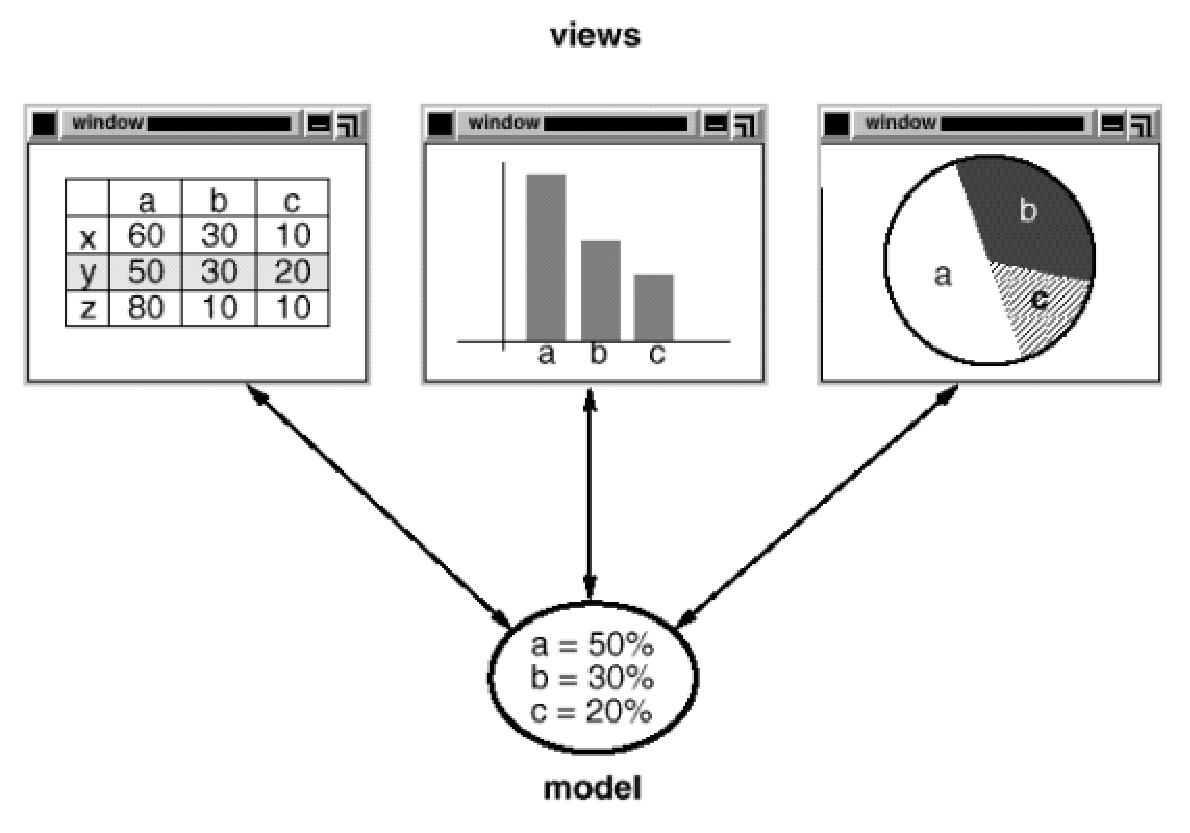
\includegraphics[width=1.0\textwidth]{img/mvc-1.pdf}
      \caption{Model-View-Controller - różna reprezentacja graficzna tych samych danych. Żródło: \cite{GoF}.}
      \label{fig:mvc-1}
    \end{figure*}

    \subsubsection{Praca z Grails}

    Struktura katalogów nowo utworzonej aplikacji Grails wygląda następująco:

    \begin{verbatim}

    + grails-app
      + conf           ---> lokalizacja artefaktów konfiguracji
        + hibernate    ---> opcjonalne pliki konfiguracyjne hibernate
        + spring       ---> opcjonalne pliki konfiguracyjne spring 
      + controllers    ---> kontrolery aplikacji
      + domain         ---> klasy reprezentujące modele
      + i18n           ---> zlokalizowane komunikaty il8n
      + services       ---> warstwa serwisowa
      + taglib         ---> biblioteki znaczników
      + util           ---> klasy pomocnicze special utility classes 
      + views          ---> lokalizacja widoków
        + layouts      ---> lokalizacja 
      + lib
      + scripts        ---> skrypty gant
      + src
      + groovy         ---> opcjonalnie, źródła groovy inne niż
                            w grails-app/*
      + java           ---> opcjonalnie, źródła java 
      + test           ---> generowane testy aplikacji
      + web-app
        + WEB-INF

    \end{verbatim}

    \subsubsection{GORM - Grails Object Relational Mapping}
  
    Po wstępnej analizie, mając wiedzę na temat dziedziny problemu, w prosty sposób można utworzyć podstawową funkcjonalność przykładowej aplikacji. Proces tworzenia elementów budowanego systemu rozpoczyna się od stworzenia klasy Groovy reprezentującej model (na przykładzie implementacji z systemu Reqmanager):

    \begin{lstlisting}[caption={klasa modelu Project.groovy}, label={lst:modelExample}]
    package pl.edu.pjwstk.reqmanager.examples
    class Project {
        String name
        String description
        String mainNote
        java.sql.Timestamp timestamp
        java.util.Date deadline

        static hasMany = [requirements:Requirement]
    }
    \end{lstlisting}

    Jeśli nie skonfigurujemy aplikacji w niestandardowy sposób, po stworzeniu powyższej klasy Groovy w katalogu grails-app/domain, Framework Grails przy pomocy Hibernate utworzy następującą strukturę w bazie danych:

    \begin{lstlisting}[caption={struktura bazy danych dla modelu Project}, label={lst:dbSchemaProject}]
                      Table "public.project"
       Column    |            Type             | Modifiers 
    -------------+-----------------------------+-----------
     id          | bigint                      | not null
     version     | bigint                      | not null
     deadline    | timestamp without time zone | 
     description | character varying(255)      | not null
     name        | character varying(255)      | not null
     timestamp   | timestamp without time zone | not null
     main_note   | character varying(255)      | 
    Indexes:
        "project_pkey" PRIMARY KEY, btree (id)
    Referenced by:
        TABLE "requirement" CONSTRAINT "fk15a8dc43ffd118f2" 
        FOREIGN KEY (project_id) REFERENCES project(id)
    \end{lstlisting}

    Powyższy przykład przedstawia, jak w prosty sposób, przy niskich nakładach pracy, programista jest w stanie zbudować szkielet aplikacji zasilanej bazą danych. Jak widać, pola klasy Groovy, zostały odpowiednio odwzorowane w strukturze danych wraz z odpowiednimi typami danych po stronie bazy.

    Na szczególną uwagę zasługuje konstrukcja w klasie Project: 

    \begin{lstlisting}[caption={relacja jeden-do-wielu}, label={lst:oneToMany}]
      static hasmany = [requirements:requirement]
    \end{lstlisting}

    W języku Groovy konstrukcja ,,[:]'' jest reprezentacją pustej tablicy asocjacyjnej - struktury danych umożliwiającej przechowywanie kolekcji par ,,klucz - wartość''. W Groovy, domyślną kolekcją inicjalizowaną przy pomocy literału ,,[:]'' jest obiekt klasy java.util.LinkedHashMap. Zatem powyższa zmienna statyczna jest referencją do obietku klasy LinkedHashMap, zawierającego jedną parę, gdzie kluczem jest ciąg znaków ,,requirements'' a wartością, jest klasa Requirement. W ten sposób Grails obsługuje relacje jeden-do-wielu. W analogiczny sposób, istnieje możliwość definiowania pozostałych rodzajów relacji, tj. jeden-do-jeden, wiele-do-wielu, etc). Konstrukcja taka, umożliwia uzyskanie listy wymagań w projekcie: 

    \begin{lstlisting}[caption={wymagania przypisane do projektu}, label={lst:requirements}]
      //pobiera z bazy projekt o id = 1
      def project = Project.get(1)

      //zwraca liste wymagan podlaczonych do projektu
      def reqs = project.requirements 
    \end{lstlisting}
    
      
    \subsubsection{Kontrolery i widoki}

    W celu połączenia konkretnych widoków z akcjami kontrolerów, konwencja Grails wymaga odpowiedniego nazewnictwa metod w klasach kontrolerów. Generalizując, należy stosować się do zasady, aby nazwa metody odpowiedzialnej za realizację wybranej akcji kontrolera, posiadała plik o tej samej nazwie, z rozszerzeniem .gsp, w odpowiednim katalogu w ścieżce grails-app/views. Poniżej zamieszczono przykład realizacji akcji ,,index'' w kontrolerze ,,ProjectController''. Wbudowany w Grails mechanizm odwzorowywania adresów URL i przekierowywania do odpowiednich akcji kontrolerów automatycznie wykrywa którą metodę należy wykonać. Zatem, po wskazaniu przeglądarce internetowej adresu http://reqmanager.heroku.com/project/index system, przez konwencję, wykryje konieczność wywołania metody ,,index'' w kontrolerze ,,ProjectController''. Z kolei po wykonaniu tej metody, (o ile programista nie zdecyduje inaczej) automatycznie wyświetlany jest widok index.gsp umieszczony w katalogu grails-app/views/project. W widoku, do wykorzystania dostępne są zmienne usatwione w tabeli asocjacyjnej, zwracanej przez kontroler (w tym przypadku, zmienna ,,project'' zawierająca referencję do listy wszystkich projektów w systemie). 


    \begin{lstlisting}[caption={widok i kontroler}, label={lst:contView}]
      // klasa kontrolera:
      package pl.edu.pjwstk.reqmanager

      class ProjectController {
        def index = { 
          return [projects : Project.list()]
        }   
      }

      //widok w pliku o nazwie index.gsp 
      //umieszczony w katalogu grails-app/views/project/
      <!DOCTYPE html>
      <html>
        <div>
        <h1>Project list</h1>
        <g:each in='${projects}' var='project'>
          Nazwa: ${project.name}<br />
          Deadline: ${project.deadline.format("dd-MM yy")}<br />
          Opis: ${project.description} 
        </g:each>
        </div>
      </html>

    \end{lstlisting}

    Należy jeszcze zwrócić uwagę na pewien detal w strukturze kodu źródłowego kontrolera. Grails dopuszcza dwa podejścia do deklarowania akcji - (1) za pomocą klasycznych metod oraz (2) przy użyciu dokmnięć (closures). Formalnie domknięcia są obiektami wiążącymi funkcję oraz środowisko w jakim ta funkcja ma działać. Jest to specyficzna kontrukcja, będącą zdefiniowanym blokiem kodu, który można przekazać jako parametr innej metodzie lub funkcji. Poniższy przykład wyjaśnia zasadę na jakiej działają domknięcia w Groovy: 
    
    \begin{lstlisting}[caption={domknięcie w Groovy}, label={lst:closure}]
      def closeAllProjects() {
        def projects = Project.list()
        projects.collect { it.open = false }
      }
    \end{lstlisting} 
    
    Powyższy kod pobiera do zmiennej ,,projects'' listę wszystkich projektów w systemie. Następnie, na liście projektów wywoływana jest metoda ,,collect''. Metoda collect (zdefiniowana w interfejsie Collection) przyjmuje jako parametr blok kodu, domknięcie. Metoda collect iteruje po wszystkich elementach zbioru na rzecz którego została wykonana i wykonuje blok kodu przekazany jej jako parametr na kolejnych elementach kolekcji, następnie zwracaja listę zmodyfikowanych przez domknięcie elementów.

    \subsection{Spring Framework i Hibernate ORM}

      Sercem Grails jest Spring Framework oraz Hibernate ORM. Obie technologie są wiodące na rynku i szeroko stosowane w komercyjnych projektach dowolnych rozmiarów. Spring jest de facto zestawem narzędzi, wzorców projektowych i bibliotek realizujących ogromną ilość funkcjonalności, mających za zadanie przyśpieszyć proces wytwarzania oprogramowania oraz w pewnym zakresie zapewnić wysoką jakość tworzonych rozwiązań. Przede wszystkim jednak, jest tzw. kontenerem Inversion Of Control (odwrócenie sterowania) \cite{MFow01}. Prócz IoC Spring Framework to potężna platforma integrująca wiele rozwiązań, takich jak webowy framework Spring MVC, biblioteki i wzorce dotyczące bezpieczeństwa (Spring Security), wrapper jdbc, transakcje (Spring JDBC Templates), etc.

      Hibernate ORM jest technologią pozwalającą na mapowanie rekordów z relacyjnych baz danych, na obiekty w systemie przy pomocy plikow konfiguracyjnych xml. W Grails, potrzeba konfiguracji warstwy ORM ogranicza się do minimum, a większość standardowych zadań można zrealizować konfigurując odpowiednio blok \emph{mapping} w klasie modelu.

  \section{Pozostałe technologie}
    \subsection{Postgresql}
      Trwałość danych w aplikacjach internetowych standardowo realizowana jest przez bazę danych. Na potrzeby prezentowanego prototypu, wykorzystano bazę danych Postgresql. Jest to obiektowo-relacyjna baza danych udostępniona na licencji Wolnego i Otwartego Oprogramowania. 

      Baza danych PostgreSQL implementuje znaczną część standardu SQL:2008 [!ref - http://www.postgresql.org/docs/9.1/static/features.html]

    \subsection{Javascript, jQuery i biblioteka jsUML2}

      Wiele funkcjonlaności zrealizowano po stronie klienta, wykorzystując język javascript. W niewielkim zakresie wykorzystano popularną bibliotekę jQuery, wspierającą realizację najczęściej pojawiających się problemów w trakcie prac nad aplikacjami intenretowymi. Jednak wykorzystanie jQuery w prototypie systemu jest marginalne i ogranicza się jedynie do zastosowania metody \emph{ajax()} ułatwiającej wykonywanie asynchronicznych wywołań serwera.

      \subsubsection{jsUML2}
        jsUML2 jest biblioteką stworzoną przez środowisko naukowe, na uniwerystecie w Kordobie. Jest to zaimplementowany w całości w języku javascript, rozbudowany zestaw klas umożliwiający tworzenie wielu rodzajów diagramów UML w przeglądarce internetowej. jsUML wykorzystuje najnowszą specyfikację języka znaczników HTML5. Obiekt \emph{canvas} oferuje szerokie spektrum możliwości programistom aplikacji internetowych. Element \emph{canvas} umożliwia programistyczne tworzenie kształtów i obrazów bitmapowych w przeglądarce internetowej. Canvas udostępnia programistom interfejs HTMLCanvasElement umożliwiający modyfikację zawartości elementów canvas w htmlu. Metoda interfejsu \emph{getContext()} zwraca tzw. ,,drawing context'' - w zależności od parametru przekazanego metodzie \emph{getContext()}, zwracany jest obiekt klasy (1) CanvasRenderingContext2D w przypadku przekazania paramteru '2d' lub (2) WebGLRenderingContext w przypadku przekazania paramteru 'experimental-webgl'.

        Poniżej zamieszczono przykładowy kod, umożliwiający rozpoczęcie pracy obiektem klasy CanvasRenderingContext2D. Wykonanie kodu spowoduje narysowanie prostokąta:

      \begin{lstlisting}[caption={przykład HTML5 canvas}, label={lst:canvas1}]
      var canvas = document.getElementById('example');
      var drawingContext = canvas.getContext('2d')

      drawingContext.fillStyle = "rgb(200,0,0)";  
      drawingContext.fillRect(10, 10, 55, 50);
      \end{lstlisting}

        Biblioteka jsUML2 składa się z dwóch pakietów klas: (1) \emph{UDCore} - zawierający bazowe klasy umożliwiające tworzenie i obsługę graficzną diagramów i komponentów pomocniczych; (2) \emph{UDModules} - zawierający faktyczną implementację diagramów standard UML, zbudowaną na bazie klas pierwotnych z pakietu \emph{core}.

        Głównymi elementami w poszczególnych pakietach są:

        \begin{itemize}
          \item UDCore
            \begin{itemize}
              \item Diagram
              \item Node (węzeł)
              \item Relation (relacja)
            \end{itemize}
          \item Modules 
            \begin{itemize}
              \item Use case diagrams
              \item Class diagrams
              \item Component diagrams
              \item Message sequence diagrams
              \item State charts
            \end{itemize}
        \end{itemize}

        Na listingu \ref{lst:UDCore} zawarto wykaz klas dostępnych w pakiecie \emph{core}:

        \begin{lstlisting}[caption={klasy bazowe jsUML2}, label={lst:UDCore}]
        AttributeFields.js
        AttributeItem.js
        CircleSymbol.js
        CollapsibleFields.js
        Component.js
        ComponentSymbol.js
        ConnectorItem.js
        DataStoreItem.js
        Diagram.js
        Dialog.js
        Element.js
        Elliptical.js
        GuardItem.js
        JSFun.js
        JSGraphic.js
        LoopItem.js
        NodeFigure.js
        Node.js
        ObjectItem.js
        OperationFields.js
        OperationItem.js
        Point.js
        Rectangular.js
        RegionItem.js
        Region.js
        RegionLine.js
        RelationEnd.js
        Relation.js
        RelationLine.js
        Rhombus.js
        RoleItem.js
        Rombo.js
        Separator.js
        Space.js
        SpecificationItem.js
        StereotypeFields.js
        StereotypeItem.js
        SuperComponent.js
        SuperNode.js
        Tab.js
        TextArea.js
        TextBox.js
        TextFields.js
        Text.js
        TransitionItem.js
        \end{lstlisting}

        W pakiecie modules, do dyspozycji programisty znajdują się następujące podpakiety klas:

        \begin{lstlisting}[caption={pakiety modułów jsUML2}, label={lst:UDModules}]
        activity
        class
        component
        generic
        profile
        sequence
        stateMachine
        usecase
        \end{lstlisting}

        W celu inicjalizacji biblioteki jsUML2, należy stworzyć odpowiednią strukturę dokumentu html:

        \begin{lstlisting}[caption={HTML canvas element}, label={lst:HTML5Ex}]
        <div id="ud_diagram_div" style="position: relative">
          <canvas id="c1" class="ud_diagram_canvas" style="position: absolute;" width="500")
          <canvas id="c2" class="ud_diagram_canvas" style="position: absolute;" width="500")
        </div>
        \end{lstlisting}
      
        Następnie, niezbędna jest inicjalizacja odpowiedniego diagramu (na przykładzie diagramu przypadków użycia):

        \begin{lstlisting}[caption={HTML canvas element - JS}, label={lst:jsCanvasEx}]
        var mainEl = document.getElementById('c1');
        var motionEl = document.getElementById('c2');

        var mainCtx = mainEl.getContext('2d');
        var motionCtx = motionEl.getContext('2d');

        var div = document.getElementById('ud_diagram_div')

        var diagram = new UMLUseCaseDiagram()

        //metoda initialize() przyjmuje kolejno parametry:
        //(1) unikalny identyfikator diagramu
        //(2) element blokowy html bedacy kontenerem diagramu
        //(3) obiekt 'context' stanowiacy 'gorna' warstwe
        //    diagramu
        //(4,5) rozmiary w pikslach 

        diagram.initialize(1, div, motionCtx, 600, 600) 
        \end{lstlisting}

\subsection{System kontroli wersji git i serwer heroku}
  
  W trakcie pracy wykorzystano system kontroli wersji \emph{git} oraz serwer heroku. 

  Git jest systemem kontroli wersji udostępnionym na licencji GPL, stworzonym przez Linusa Torvaldsa w 2005 roku. Głównymi założeniami projektu były szybkość działania, bezpieczeństwo oraz rozwiązanie problemów jakie twórca uważał są najbardziej rażące w systemach CSV oraz SVN.

  Heroku udostępnia platformę hostingową obsługującą wiele języków programowania. Zasada działa serwerów Heroku, oparta jest na koncepcji utrzymania aplikacji w ,,chmurze'' serwerów - infrastruktura sprzętowa jest niewidoczna dla użytkowników. Użytkownicy tej usługi wykupują moc obliczeniową serwerów odpowiadającą potrzebom utrzymywanych aplikacji, płacąc za czas dostępu do serwerów o wybranej mocy obliczeniowej. Główną zaletą tego rozwiązania jest możliwość natychmiastowego skalowania aplikacji w zależności od zapotrzebowania na moc obliczeniową. W przypadku znacznego wzrostu ruchu na serwerze, użytkownik może wykupić dodatkową moc obliczeniową, bez konieczności przerywania ciągłości działania usługi w sieci. Heroku udostępnia swoją infrastrukturę w podstawowym zakresie, bez konieczności uiszczania opłat, dlatego jest to rewelacyjne rozwiązania na potrzeby testów i prezentacji aplikacji internetowych. Dzięki natywnemu wsparciu systemu kontroli wersji Git, instalacja aplikacji w chmurze, polega na przesłaniu na serwer aktualizacji kodu źródłowego i wykonania polecenia inicjalizującego instalację kodu na serwerze heroku:


        \begin{lstlisting}[caption={}, label={lst:jsCanvasEx}]
        ~$ git add .
        ~$ git commit -m 'update'
        ~$ git push origin master
        \end{lstlisting}

\subsection{Środowisko programistyczne (Linux, vim)}

  Do stworzenia zarówno prorotypu aplikacji, jak i do edycji i składu części tekstowej niniejszej pracy, wykorzystano zasadniczo narzędzia dostępne w systemie operacyjnym Linux (Ubuntu Linux v11.10). 

  Do edycji kodu źródłowego wykorzystano klasyczny edytor tekstowy vim z zainstalowanym dodatkiem ułatwiającym poruszanie się w strukturze katalogów grails (vim grails plugin z zainstalowanym dodatkiem ułatwiającym poruszanie się w strukturze katalogów grails (vim grails plugin).

  Część opisowa niniejszej pracy również powstała w edytorze tekstu vim. Do składu tekstu zastosowano popularne oprogramowanie \LaTeX. 

  \chapter{Rozwiązania implementacyjne}
  
  W poprzednim rozdziale opisano narzędzia jakie wykorzystano w trakcie budowy prototypu. W niniejszym rozdziale, przedstawiono zastosowane konkretne rozwiązania implementacyjne. Szczególną uwagę zwrócono na moduł edycji diagramów przypadków użycia oraz generator specyfikacji wymagań.

  \section{Architektura systemu}

    System Reqmanager zbudowany jest w oparciu o, opisaną w rozdziale 4, technologię Grails, integrującą wiele istniejących rozwiązań zbudowanych na bazie wirtualnej maszyny Javy. Na Rysunku \ref{fig:techstack} przedstawiono ogólną architekturę Grails.

    \begin{figure*}[h]
      \centering
      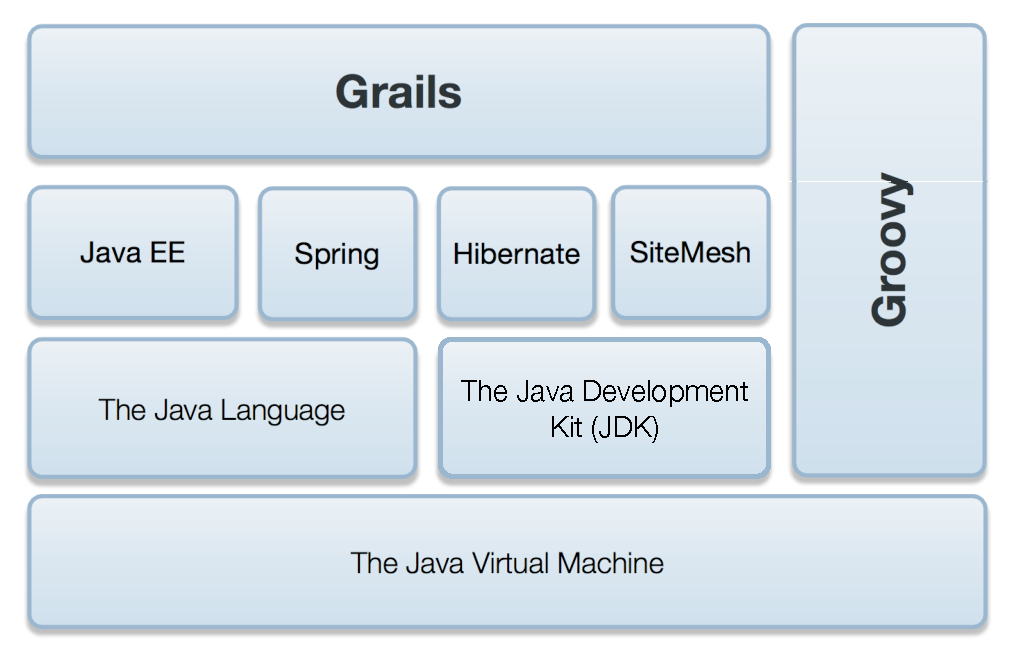
\includegraphics[width=1.0\textwidth]{img/grails-stack-rev2.pdf}
      \caption{Architektura Grails}
      \label{fig:techstack}
    \end{figure*}
     
    Definiowanie wymagań w systemie Reqmanager polega na jednoczesnym dostępie do edytora tekstu oraz edytora diagramów przypadków użycia. Użytkownik, mając otwartą aplikację, oprócz tekstowego opisu wymagania, ma możliwość dodawania oraz edycji przypadków użycia w formie graficznej.

    Aplikacja Reqmanager jest typową aplikacją internetową typu klient-serwer, gdzie klientem jest przeglądarka użytkownika korzystającego z aplikacji zainstalowanej na zdalnym serwerze, odpowiednio reagującej na żądania klienta na zasadzie żądanie - odpowiedź (request - response). Przeglądarka internetowa jest tak zwanym ,,cienkim klientem'' z racji silnego uzależnienia działania od serwera aplikacji. Na Rysunku \ref{fig:reqarch} przedstawiono poszczególne moduły proponowanego systemu wraz z podziałem na warstwy.
 
    Na potrzeby aplikacji Reqmanager, utworzono następującą strukturę modeli aplikacji:

    \begin{figure*}[p]
      \centering
      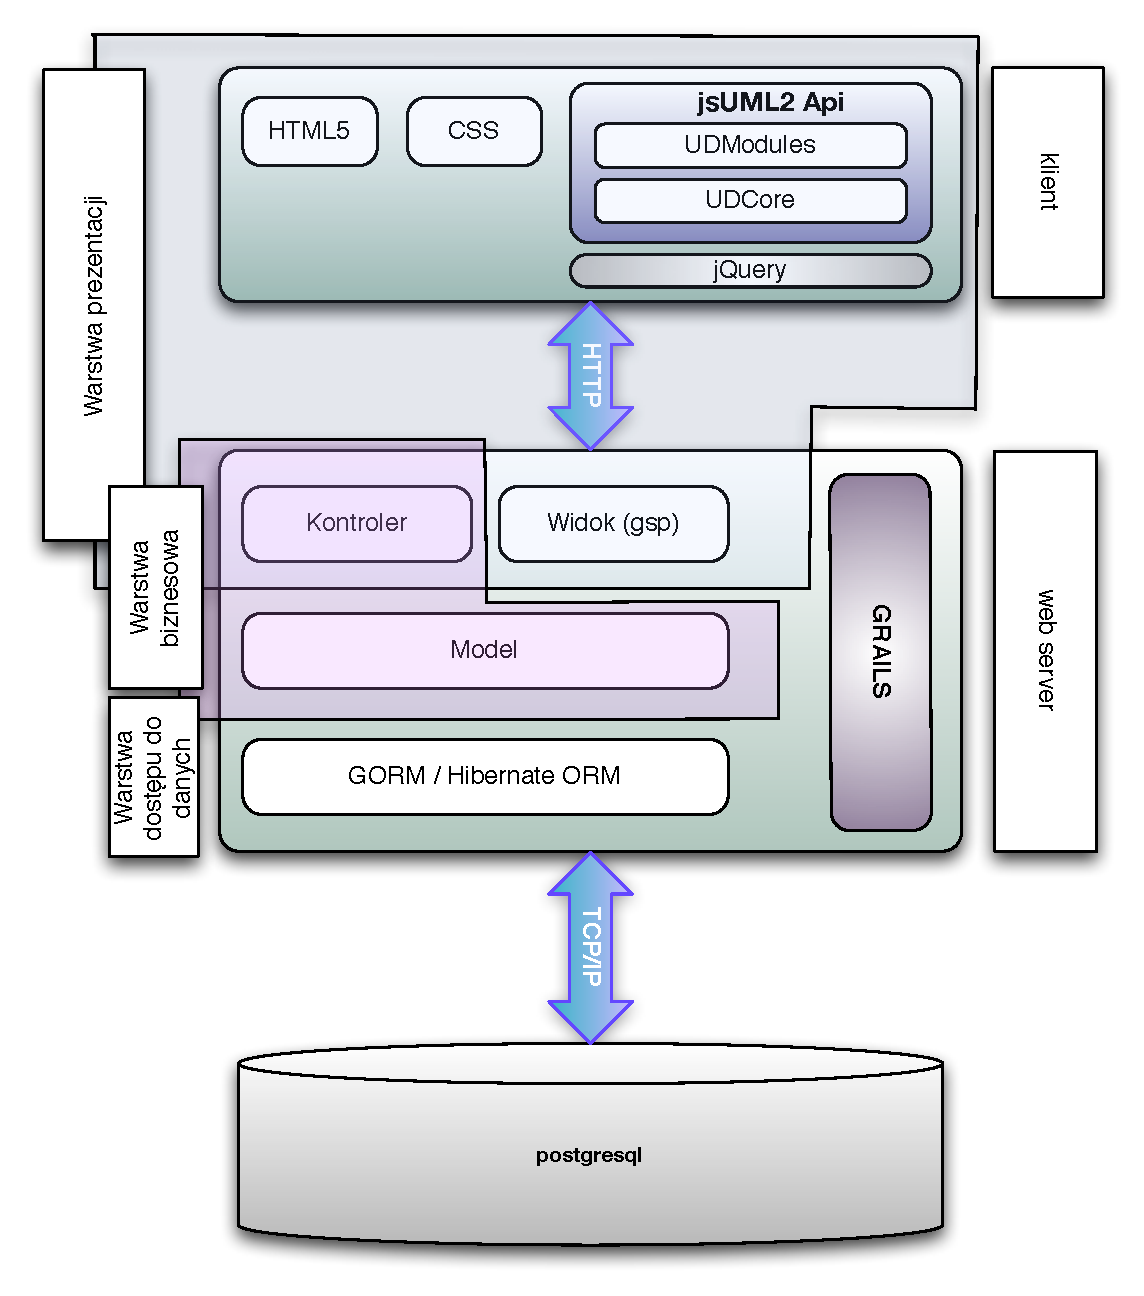
\includegraphics[width=1.0\textwidth]{img/reqmanager.pdf}
      \caption{Ogólna architektura systemu}
      \label{fig:reqarch}
    \end{figure*}

    \begin{verbatim}
    Diagram 
    Project
    Requirement
    UseCase
    \end{verbatim}

    Struktura bazy danych jest generowana automatycznie, na podstawie analizy klas modeli. Diagram utworzonej bazy, przedstawiono na rysunku \ref{fig:erd1}

    \begin{figure*}[p]
      \centering
      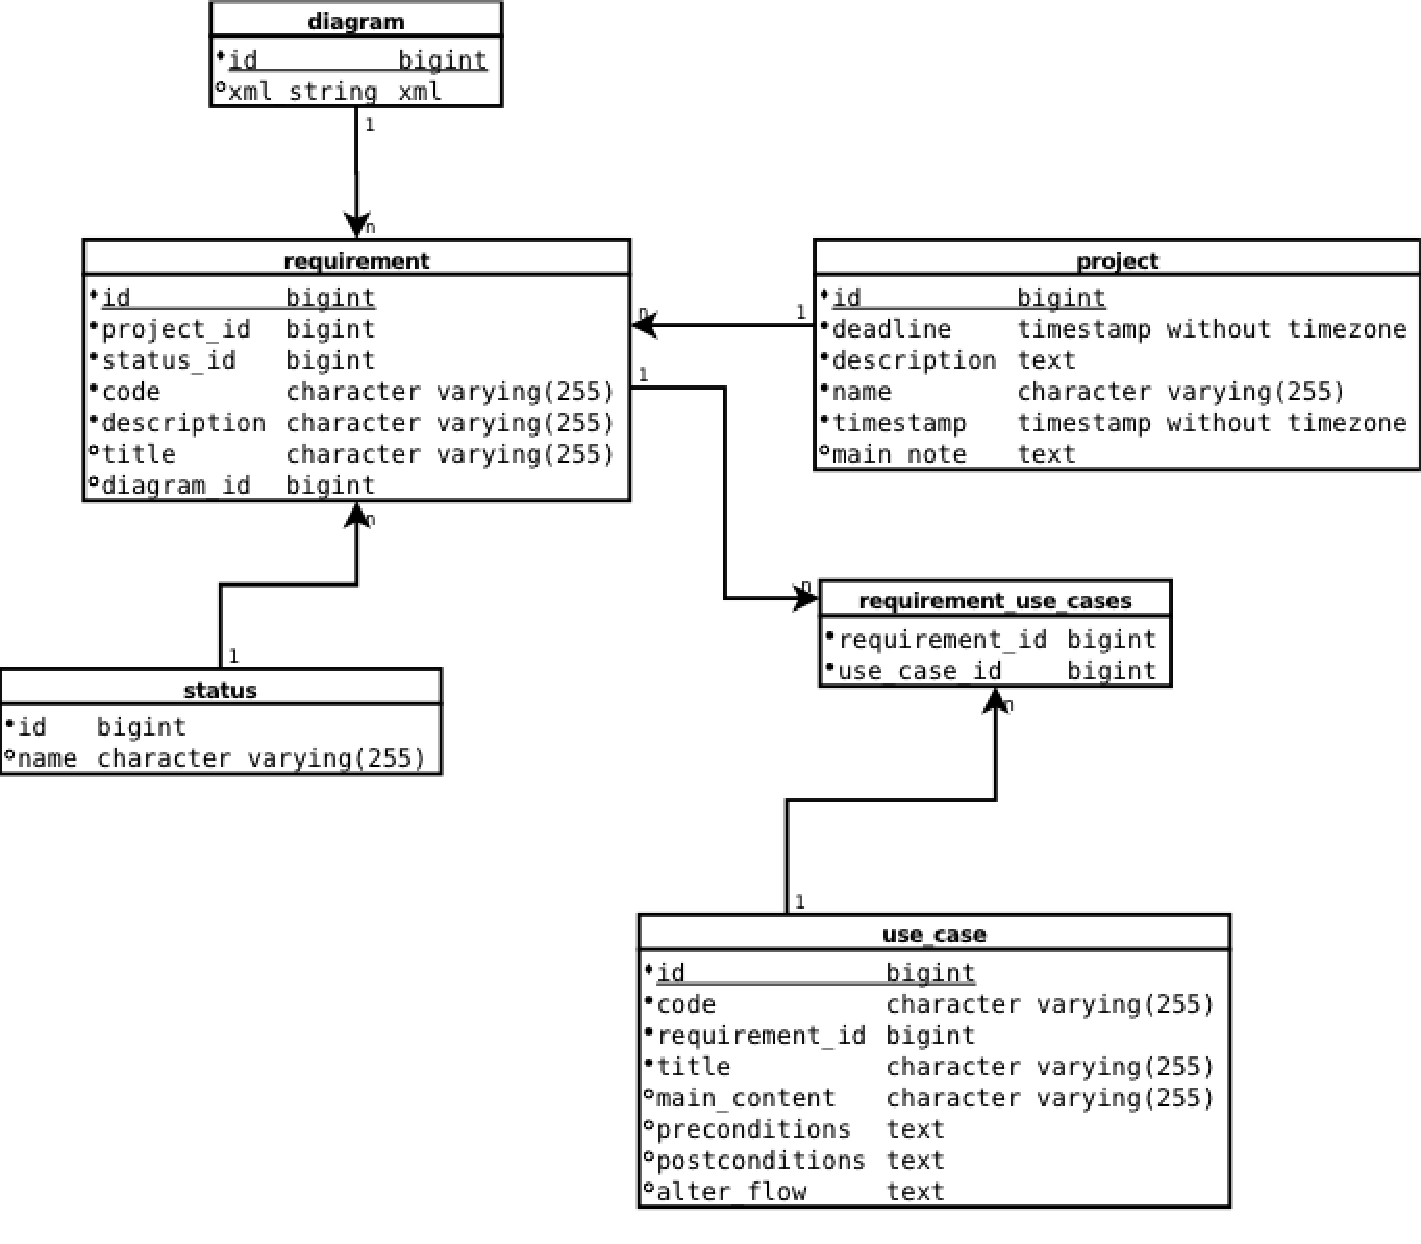
\includegraphics[width=1.0\textwidth]{img/erd2.pdf}
      \caption{Diagram struktury bazy danych systemu Reqmanager}
      \label{fig:erd1}
    \end{figure*}

  \section{Funkcjonalności systemu}

    Poniżej opisano poszczególne funkcjonalności proponowanego rozwiązania wraz z przykładami realizacji w kodzie.
  
    \subsection{Tworzenie diagramów}

      Diagramy przypadków użycia w systemie edytowane są po stronie klienta, dzięki wykorzystaniu elementu \emph{canvas} wprowadzonego niedawno do specyfikacji języka HTML5. Obsługa tej funkcjonalności po stronie przeglądarki, stanowi problem związany z zapisem stanu diagramu. W celu rozwiązania tego problemu, zaimplementowano mechanizm serializacji stanu elementów diagramu w formacie xml do bazy danych. Cel ten osiągnięto, wykorzystując metodę \emph{getXMLString()} udostępnioną przez wszystkie obiekty dziedziczące po klasie \emph{Diagram} w bibliotece jsUML2. Przykładową strukturę zserializowanego diagramu, umieszczono na Listingu \ref{lst:diagramXml}. 
      Dodanie nowego diagramu wiąże się zatem z inicjalizacją i wyświetleniem użytkownikowi obszaru roboczego diagramu bez komunikacji z serwerem. Diagram tworzony jest po załadowaniu widoku edycji wymagania, jak pokazano na Listingu \ref{lst:appUseCase}:

      \begin{lstlisting}[caption={Widok requriement/edit.gsp}, label={lst:appUseCase}]
      window.onload = function() {
        var app = new AppUseCase("ud_diagram_div");
      }

      \end{lstlisting}

      \newpage

      AppUseCase jest obiektem JavaScript typu singleton, którego skrócona implementacja została przedstawiona na Listingu \ref{lst:appUseCaseImpl}: 
    
      \begin{lstlisting}[caption={Implementacja obiektu JS AppUseCase}, label={lst:appUseCaseImpl}]
      var AppUseCase = function(elementId) { 
        var xmlstr = document.getElementById('diagramXml').value
        var ucDiag = new UMLUseCaseDiagram() 
        if(xmlstr) {
          ucDiag.setXMLString(xmlstr);
        }

        var c1 = document.getElementById('c1');
        var c = c1.getContext('2d');
        var c2 = document.getElementById('c2');
        c2.onmousedown = function() { return false; };
        var mc = c2.getContext('2d')}

        var div = document.getElementById('ud_diagram_div');

        ucDiag.initialize(11, div, c, mc, 600, 1000);
        ucDiag.draw();
      }
      \end{lstlisting}

      Powyższy kod JavaScript, pobiera wartość z elementu formularza i identyfikatorze ,,diagramXml'' oraz tworzy nowy obiekt UMLUseCaseDiagram, zdefiniowany w pakiecie \emph{modules} biblioteki jsUML2. Następnie weryfikuje czy pole \emph{diagramXml} jest niepuste. Jeśli warunek jest prawdziwy, wywołuje metodę \emph{setXMLString()} na obiekcie diagramu, dzięki czemu diagram inicjalizowany jest z wartościami wcześniej zserializowanymi do formatu xml i zapisanymi w bazie danych. Kolejne wiersze zajmują się utworzeniem kontekstów na bazie elementów \emph{canvas}, aby na końcu zainicjować i narysować odpowiedni diagram w oknie przeglądarki użytkownika. Należy jednocześnie zaznaczyć, iż w przypadku, gdy nie istnieje zserializowana wersja diagramu w bazie (pole \emph{diagramXml} jest puste), wówczas zostanie zainicjalizowany nowy, pusty diagram, nieposiadający żadnych elementów. 

      \subsubsection{Zapis danych xml}

      Dopiero gdy użytkownik wybierze opcję zapisu aktualnego wymagania, zserializowany stan diagramu w formacie xml, zostanie przesłany metodą POST do serwera. Następnie otrzymany po stronie serwera ciąg znaków xml zostanie przetworzony, utworzony zostanie obiekt klasy Diagram i na końcu nastąpi zapis obiektu do bazy danych. Za ten proces odpowiedzialna jest akcja \emph{save} kontrolera \emph{Requirement}. Jest to dość ograniczone rozwiązanie, które można byłoby usprawnić wprowadzając asynchroniczny, automatyczny zapis stanu diagramu co kilka sekund lub po każdej aktualizacji po stronie klienta.

      \begin{lstlisting}[caption={Struktura xml diagramu}, label={lst:diagramXml}]

      <UMLUseCaseDiagram name="Use case diagram">
        <UMLSystem id="UMLSystem_4" x="165" y="97" ... >
          <superitem id="stereotypes" visibleSubComponents="true"/>
          <item id="name" value="System name"/>
          <UMLUseCase id="UMLUseCase_1" x="232" y="142" ... >
            <superitem id="stereotypes" visibleSubComponents="true"/>
            <item id="name" value="test test"/>
          </UMLUseCase>
          <UMLUseCase id="UMLUseCase_3" x="222" y="209" ... >
            <superitem id="stereotypes" visibleSubComponents="true"/>
            <item id="name" value="for req 74"/>
          </UMLUseCase>
        </UMLSystem>
      </UMLUseCaseDiagram>

      \end{lstlisting}

      Baza danych PostgreSQL obsługuje specjalny typ danych ,,xml''. Dzięki temu, po stronie bazy dokonywana jest weryfikacja poprawności dokumentu jaki programista ma zamiar zapisać. Niestety Framework Grails nie współpracuje dobrze z taką konstrukcją, dlatego niezbędna była implementacja rozwiązania rzutującego typ \emph{String} na typ \emph{SQLXMLType}. W tym celu została stworzona specjalna klasa w Javie, implementująca interfejs \emph{org.hibernate.usertype.UserType} (patrz Listing \ref{lst:xmlType}). Hibernate udostępnia ten interfejs umożliwiając programistom tworzenie własnych typów danych i zdefiniowanie ich zachowania w stosunku do bazy. Dodatkowo, niezbędne było odpowiednie przygotowanie modelu, podając typ pola przechowującego xml jako String, a następnie stworzyć odpowiedni blok ,,mapping'' w modelu. Na Listingu \ref{lst:xml}, dla przykładu zaprezentowano implementację klasy Diagram z systemu Reqmanager:
 
      \begin{lstlisting}[caption={Implementacja niestandardowego typu SQLXMLType}, label={lst:xmlType}]
      package pl.edu.pjwstk.reqmanager
       
      import java.io.Serializable;
      import java.sql.PreparedStatement;
      import java.sql.ResultSet;
      import java.sql.SQLException;
      import java.sql.Types;
      import org.hibernate.HibernateException;
       
      /**
       * Store and retrieve a PostgreSQL "xml" column as a Java string.
       */
      public class SQLXMLType implements org.hibernate.usertype.UserType {
       
          private final int[] sqlTypesSupported = new int[] { Types.VARCHAR };
       
          @Override
          public int[] sqlTypes() {
              return sqlTypesSupported;
          }
       
          @Override
          public Class returnedClass() {
              return String.class;
          }
       
          @Override
          public boolean equals(Object x, Object y) throws HibernateException {
              if (x == null) {
                  return y == null;
              } else {
                  return x.equals(y);
              }
          }
       
          @Override
          public int hashCode(Object x) throws HibernateException {
              return x == null ? null : x.hashCode();
          }
       
          @Override
          public Object nullSafeGet(ResultSet rs, String[] names, Object owner) throws HibernateException, SQLException {
              assert(names.length == 1);
              String xmldoc = rs.getString( names[0] );
              return rs.wasNull() ? null : xmldoc;
          }
       
          @Override
          public void nullSafeSet(PreparedStatement st, Object value, int index) throws HibernateException, SQLException {
              if (value == null) {
                  st.setNull(index, Types.OTHER);
              } else {
                  st.setObject(index, value, Types.OTHER);
              }
          }
       
          @Override
          public Object deepCopy(Object value) throws HibernateException {
              if (value == null)
                  return null;
              return new String( (String)value );
          }
       
          @Override
          public boolean isMutable() {
              return false;
          }
       
          @Override
          public Serializable disassemble(Object value) throws HibernateException {
              return (String) value;
          }
       
          @Override
          public Object assemble(Serializable cached, Object owner) throws HibernateException {
              return (String) cached;
          }
       
          @Override
          public Object replace(Object original, Object target, Object owner) throws HibernateException {
              return original;
          }
      }
      \end{lstlisting}

      \newpage

      \begin{lstlisting}[caption={Implementacja modelu Diagram}, label={lst:xml}]
      package pl.edu.pjwstk.reqmanager
      public class Diagram {
        String name
        String xmlString

        static belongsTo = Requirement
        static mapping = {
          xmlString type: SQLXMLType
        }
        static constraints = {
          name(nullable:true)
        }
      }
      \end{lstlisting}

    \subsection{Współdzielenie diagramów}

    Istotnym elementem systemu jest współdzielenie diagramów między wieloma wymaganiami. Każdy diagram może zostać przypisany do kilku wymagań. Wówczas modyfikacja przypadków użycia w trakcie edycji konkretnego wymagania, wiąże się z aktualizacją stanu diagramu we wszystkich korzystających z niego miejscach w systemie.
    
    \subsection{Mapowanie przypadków użycia}
      W związku z możliwością współdzielenia diagramów pomiędzy wieloma wymaganiami, w aktualnej wersji prototypu, przypadki użycia są łączone z wymaganiem, tylko po wykonaniu przez użytkownika akcji wskazania przypadku użycia jako realizującego aktualnie modyfikowane wymaganie.

      Na etapie edycji diagramu, użytkownik ma możliwość wskazania konkretnych use case'ów znajdujących się na diagramie, jako odpowiedzialnych za realizację wybranego wymagania. Powiązanie przypadku użycia z wymaganiem polega na wyborze opcji \emph{mark for requirement} z paska narzędzi diagramu, a następnie kliknięciu w dany przypadek użycia na diagramie. Po zatwierdzeniu operacji, zostaje wysłane asynchroniczne żądanie do serwera, pod adres http://reqmanager.herokuapp.com/requirement/\\addUseCase/id\_wymagania. W żądaniu przekazywane są do serwera parametry niezbędne dla zestawienia przypadku użycia z wymaganiem. Poniżej zamieszczono listę tych parametrów:

    \begin{itemize}
      \item \emph{id} - identyfikator wymagania do którego dodawany jest przypadek użycia
      \item \emph{clickedUCName} - nazwa przypadku użycia wprowadzona przez użytkownika
      \item \emph{clickedUCId} - identyfikator przypadku użycia wygenerowany automatycznie przez bibliotekę jsUML2
    \end{itemize}

    Asynchronicznie wysłane do serwera żądanie zostaje przekazane wraz z paramterami do akcji \emph{addUseCase} kontrolera \emph{Requirement}. Kod odpowiedzialny za połączenie przypadku użycia z wymaganiem, został załączony na Listingu \ref{lst:addUseCase}.

    \begin{lstlisting}[caption={Kod łączący przypadek użycia z wymaganiem}, label={lst:addUseCase}]
    def addUseCase = {
      def requirement = Requirement.get(params.id)
      def useCase = UseCase.findByTitle(params.clickedUCName)
      if(useCase == null) {
        useCase = new UseCase(title: params.clickedUCName, code: params.clickedUCId)
          requirement.addToUseCases(useCase)
          render(text: "ok")
      } else {
        if(!requirement.useCases.contains(useCase)) {
          requirement.addToUseCases(useCase)
          render(text: "ok")
        } 
      }
    }
    \end{lstlisting}

    Jak można odczytać z powyższego kodu źródłowego, akcja ta, pobiera odpowiednie wymaganie oraz podejmuje próbę znalezienia przypadku użycia po nazwie. Jeśli dany przypadek użycia nie istnieje jeszcze w bazie danych (nowo utworzony przypadek użycia), zostaje swtorzony nowy obiekt klasy UseCase z odpowiednimi parametrami (nazwa nadana przez użytkownika oraz identyfikator wygenerowany po stronie klienta). W przeciwnym razie, zostaje on dodany do listy przypadków użycia połączonych asocjacją z danym wymaganiem, o ile nie istnieje już na tej liście. 

    \subsection{Przypadki użycia a wymagania}
    
      W celu odpowiedniego oznaczenia przypadków użycia przypisanych do wybranego wymagania, zaimplementowano algorytm dwustopniowej inicjalizacji diagramu. Pierwszym krokiem jest ekstrakcja z bazy danych odpowiedniego wymagania, weryfikacja czy jest do niego przypisany diagram oraz czy istnieją dla niego jakieś przypadki użycia. Na podstawie tych informacji, ładowany jest widok \emph{requirement/show.gsp}. Następnie, po załadowaniu strony uruchamiany jest skrypt po stronie klienta, odwołujący się asynchronicznie z powrotem do serwera z ,,pytaniem'' o nazwy przypadków użycia przypisanych do danego wymagania. Następnie, do pamięci ładowana jest struktura xml diagramu. Program iteruje po wszyskich węzłach w poszukiwaniu pokrywających się przypadków użycia. Jeśli znajdzie choć jeden, zmienia kolor jego tła na żółty. Listing \ref{lst:colorUC} przedstawia implementację tego algorytmu.
      
    
    \begin{lstlisting}[caption={Mechanizm oznaczania przypadku użycia przypisanego do aktualnie otwartego wymagania}, label={lst:colorUC}]
    var reqUseCases = $.ajax({
      type: "GET",
      url: "http://reqmanager.herokuapp.com/requirement/getUseCases/" + reqId,
      cache: false
    }).done(function(xht){ 
      var dom = (new DOMParser()).parseFromString(diag.diagram.getXMLString(), "text/xml");
      var documentEle = dom.documentElement;
      var usecaseArray = documentEle.getElementsByTagName('UMLUseCase');

      for(var i = 0; i < usecaseArray.length; i++) {
        for(var j = 0; j < usecaseArray[i].childNodes.length; j++) {
          var itemValue = usecaseArray[i].childNodes[j].attributes.value;
          if(itemValue != undefined) {
            if(xht.indexOf(itemValue.value.toString()) != -1) {
              var divv = document.getElementById("ud_diagram_div");
              var foundUseCase = null;

              for(var k = 0; k < diag.diagram._nodes.length; k++) {
                if(diag.diagram._nodes[k].getName().toString() 
                  === xht[xht.indexOf(itemValue.value.toString())]) {
                  foundUseCase = diag.diagram._nodes[k]; 
                }
              };
              if(foundUseCase) foundUseCase.setBackgroundColor("#F3F5BC");
              diag.diagram.draw();
            }
          }
        }
      }
    });
    \end{lstlisting}

    \newpage

    \subsection{Edytor tekstu}
      W celu ułatwienia użytkownikowi pracy z tekstem, zaimplementowano edytor, oparty na bibliotece Ace Editor. 
      Kod inicjujący edytor tekstu, znajduje się na Listingu \ref{lst:editorInit}.

    \begin{lstlisting}[caption={Inicjalizacja edytora tekstu}, label={lst:editorInit}]
    var editor = ace.edit("description");
    var MarkdownMode = require("ace/mode/markdown").Mode;
    editor.setTheme("ace/theme/clouds_midnight");
    editor.getSession().setMode(new MarkdownMode());
    editor.getSession().setUseWrapMode(true);
    \end{lstlisting}

    Kod z Listingu \ref{lst:editorInit} inicjuje edytor, załączając go do wskazanego węzła w dokumencie html (w tym przypadku jest to warstwa ,,description''). Następnie ustawia wygląd graficzny edytora oraz przestawia go w tryb pracy z formatem Markdown.
    Zawartość edytora tekstu, przekazywana jest do serwera po wysłaniu formularza przez użytkownika. Ponieważ zawartość formularza znajduje się w elemencie \emph{div} w strukturze DOM strony, w celu przekazania jego wartości, jest ona kopiowana do specjalnego pola typu textarea. Proces ten zaprezentowano na Listingu \ref{lst:txtCopy}.

    \begin{lstlisting}[caption={Kopiowanie zawartości edytora tekstu do pola textarea}, label={lst:txtCopy}]
    $("#submitbtn").click(function() {
      textarea.val(editor.getSession().getValue()); 
      $("#diagramXml").val(app.diagram.getXMLString());
    });
    \end{lstlisting} 

    \subsection{Generowanie dokumentacji}
      
      W prototypie zaimplementowano mechanizm generowania specyfikacji wymagań przy użyciu bibliotek MarkdownJ oraz iText.

      MarkdownJ jest napisaną w Javie implementacją konwertera tekstu do formatu HTML. Jest to bardzo prosta biblioteka, w której główną klasą jest \emph{MarkdownProcessor}. Metoda \emph{markdown()} przymuje jako parametr ciąg znaków (sformatowany znacznikami Markdown). W odpowiedzi zwracana jest ta sama treść, osadzona w odpowiedniej strukturze HTML. Przykładowy kod konwertujący przedstawiono na Listingu \ref{lst:markdownProc}.

      \begin{lstlisting}[caption={Wykorzystanie klasy MarkdownProcessor}, label={lst:markdownProc}]
      def m = new MarkdownProcessor(); 
      StringBuffer sb = new StringBuffer()
      sb.append("# Example header in Markdown")
      sb.append("\n")
      sb.append("This will render as a regular '<p>' paragraph")
      String html = m.markdown(sb.toString()); 
      \end{lstlisting}

      iText z kolei, jest zaawansowaną biblioteką wykorzystywaną do generowania wszelkiego rodzaju dokumentów PDF bezpośrednio z kodu Javy. W pracy wykorzystano klasę \emph{ITextRenderer} dostępną w pakiecie org.xhtmlrenderer.pdf. Pozwala ona na generowanie dokumentów PDF w oparciu o strukturę XHTML. Połączenie MarkdownJ z biblioteką iText idealnie spełnia wymagania systemu w zakresie automatycznego tworzenia specyfikacji.

      Generowanie specyfikacji w systemie przebiega w dwóch krokach. W pierwszej kolejności zostają pobranie niezbędne informacje z bazy danych dotyczące wybranego projektu, a zawartość poszczególnych pól, zostaje przekazana do klasy MarkdownToHTML konwertującej tekst do HTML. Następnie, zwrócona struktura jest przekazywana klasie ITextRenderer w celu wygenerowania dokumentu PDF. Zwrócony strumień danych zostaje wysłany do klienta jako odpowiedź serwera, co skutkuje możliwością zapisu pliku PDF na komputerze klienckim. Proces ten zobrazowany został na diagramie sekwencji, załączonym na Rysunku \ref{fig:seq}.

      \begin{figure*}[t]
        \centering
        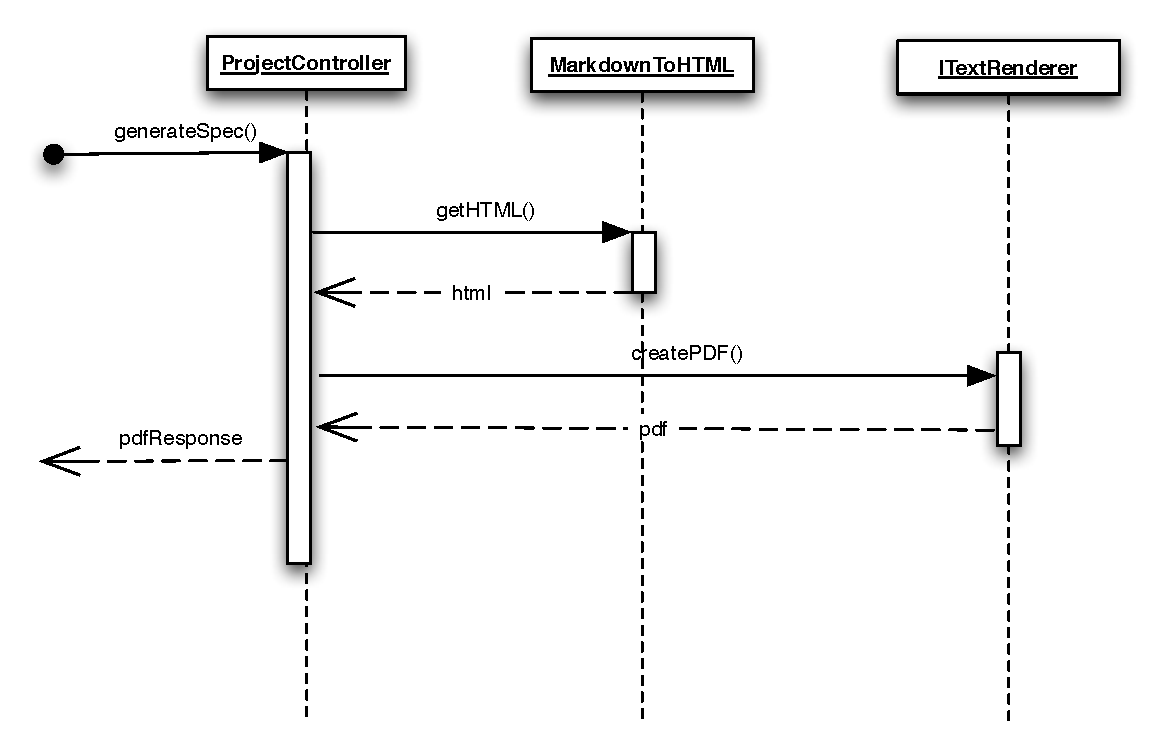
\includegraphics[width=1.0\textwidth]{img/seq.pdf}
        \caption{Generowanie dokumentu pdf specyfikacji}
        \label{fig:seq}
      \end{figure*}

      \newpage

  \section{Przykład zastosowania}
    
    W tej sekcji opisano przykład zastosowania proponowanego narzędzia.

    \subsection{Ekran główny}
      
      Ekranem głównym systemu jest przegląd wszystkich projektów, przedstawiony na Rysunku \ref{fig:mainView}. Przy każdym projekcie zawarte są podstawowe informacje na jego temat, takie jak nazwa, data zakończenia, krótki opis, ilość wymagań oraz przypadków użycia. Ponadto dostępne są trzy przyciski: (1) odnośnik do szczegółów projektu, (2) odnośnik do edycji projektu, (3) przycisk generujący aktualną wersję specyfikacji wymagań. 

      \begin{figure*}[t]
        \centering
        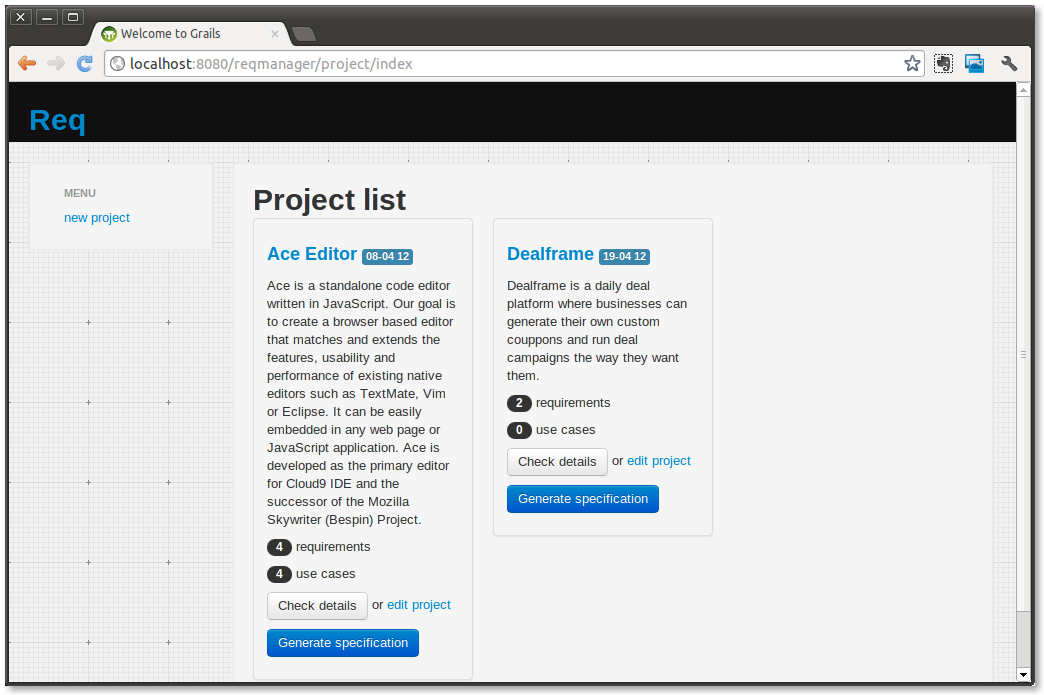
\includegraphics[width=1.0\textwidth]{img/tut_screen_1.png}
        \caption{Ekran główny projektu}
        \label{fig:mainView}
      \end{figure*}

    \subsection{Nowy projekt}
    
      Dodanie nowego projektu polega na wypełnieniu prostego formularza zawierającego informacje o nazwie, dacie zakończenia prac, krótkim opisie oraz głównej notatce. Rysunek \ref{fig:addProj} przedstawia ekran zakładania projektu.

      \begin{figure*}[t]
        \centering
        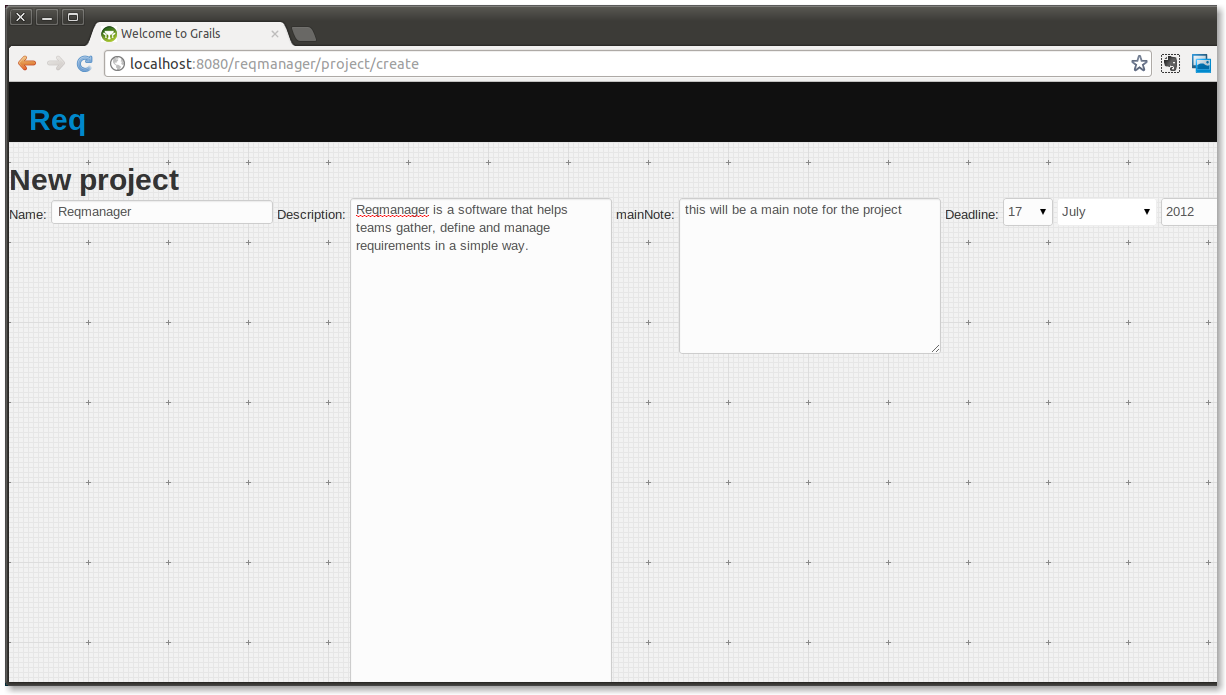
\includegraphics[width=1.0\textwidth]{img/tut_2.png}
        \caption{Dodawanie nowego projektu}
        \label{fig:addProj}
      \end{figure*}

    \subsection{Pierwsze wymaganie}

      Do nowo utworzonego projektu, można natychmiast rozpocząć dodawanie wymagań. Widok dodawania pierwszego wymagania załączono na Rysunku \ref{fig:addReq}. W tym miejscu, użytkownik ma możliwość podjęcia decyzji dotyczącej ponownego wykorzystania już istniejącego diagramu lub stworzenia nowego. Rysunek \ref{fig:addReq} przedstawia stan aplikacji po stworzeniu nowego diagramu, dodaniu pierwszego aktora, elementu granicy systemu i jednego przypadku użycia. W kolejnych widokach zaprezentowano współdzielenie diagramów.

      \begin{figure*}[t]
        \centering
        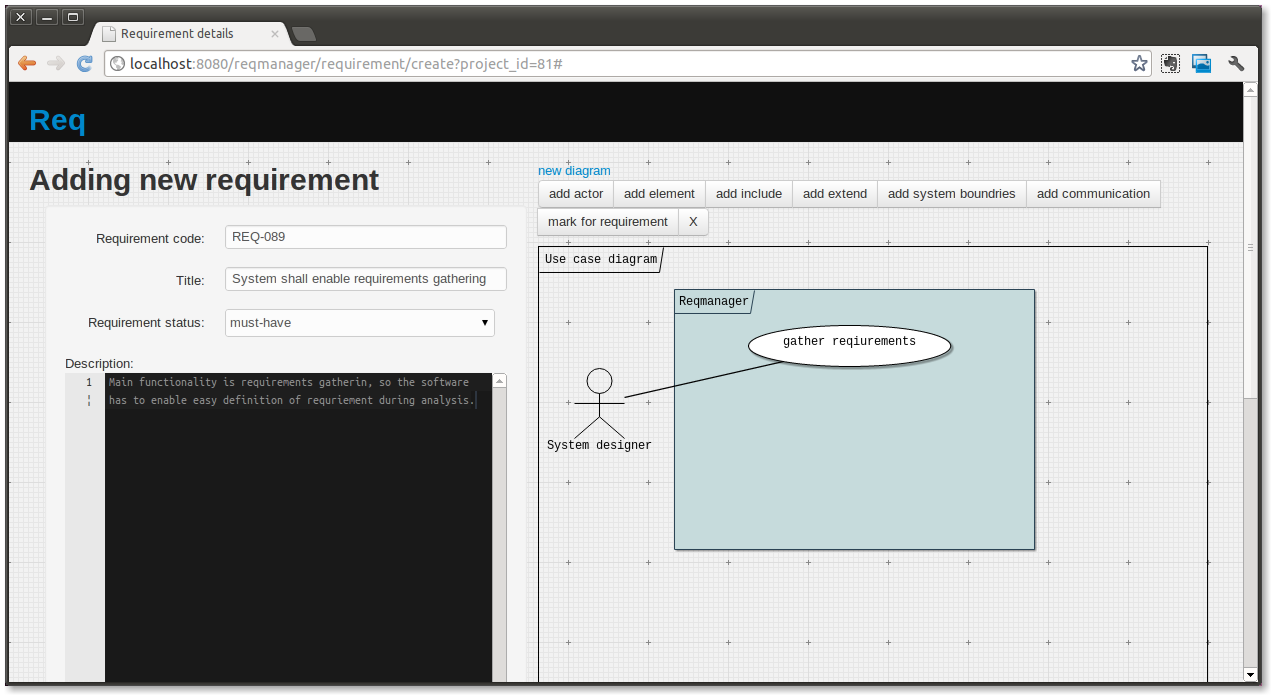
\includegraphics[width=1.0\textwidth]{img/tut_3.png}
        \caption{Definicja wymagania}
        \label{fig:addReq}
      \end{figure*}

    \subsection{Przegląd projektu}

      Rysunek \ref{fig:afterAddReq} przedstawia stan systemu po dodaniu jednego wymagania. Za pośrednictwem tego ekranu, użytkownik ma możliwość kontynuacji pracy nad główną notką projektową (i łatwy zapis tego pola za pomocą przycisku ,,Update'' umieszczonego w widocznym, dostępnym miejscu) lub dodania kolejnego wymagania.

      \begin{figure*}[t]
        \centering
        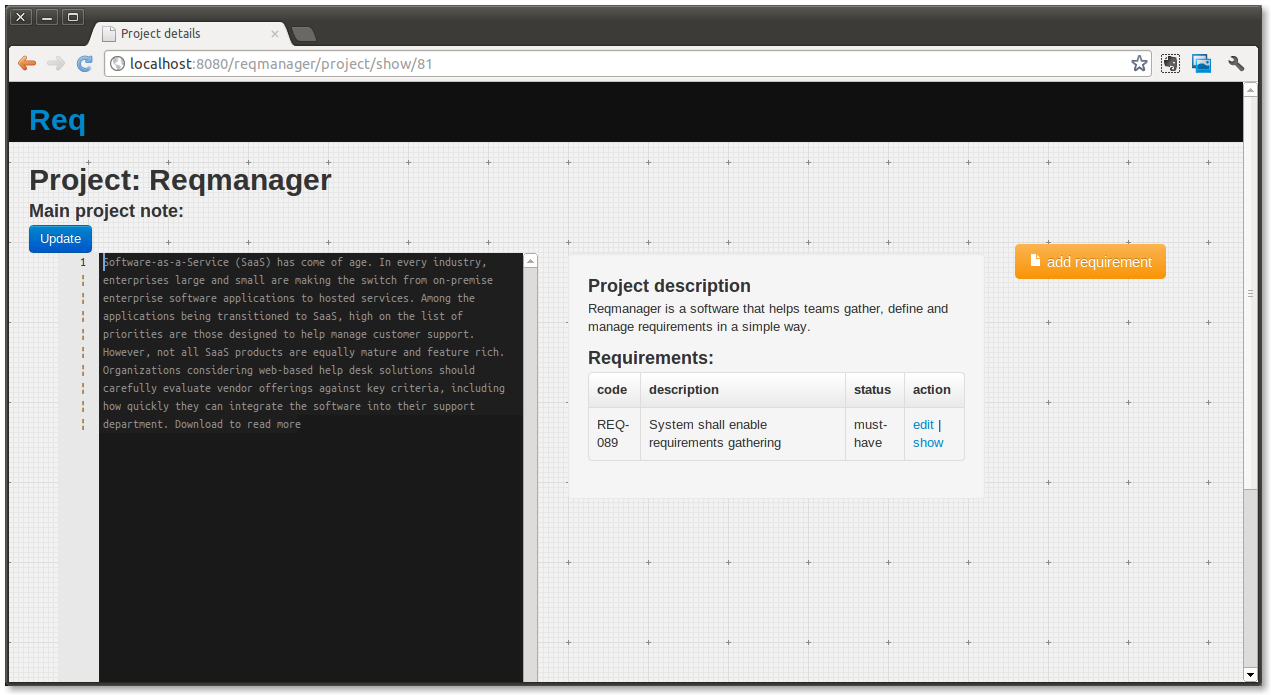
\includegraphics[width=1.0\textwidth]{img/tut_4.png}
        \caption{Stan systemu po dodaniu pierwszego wymagania}
        \label{fig:afterAddReq}
      \end{figure*}
      
    \subsection{Współdzielenie wymagań}

      Podczas dodawania kolejnych wymagań, użytkownik ma możliwość skorzystania z już istniejącego diagramu, co zaprezentowano na Rysunku \ref{fig:diagReuse}. Zamiast tworzenia nowej instancji diagramu, użytkownik ma możliwość wskazania istniejącego obiektu, który zostanie przypisany do aktualnie definiowanego elementu. Rysunek \ref{fig:diagReuse} zawiera również przykład zastosowania podstawowej składni Markdown w opisie wymagania.

      \begin{figure*}[t]
        \centering
        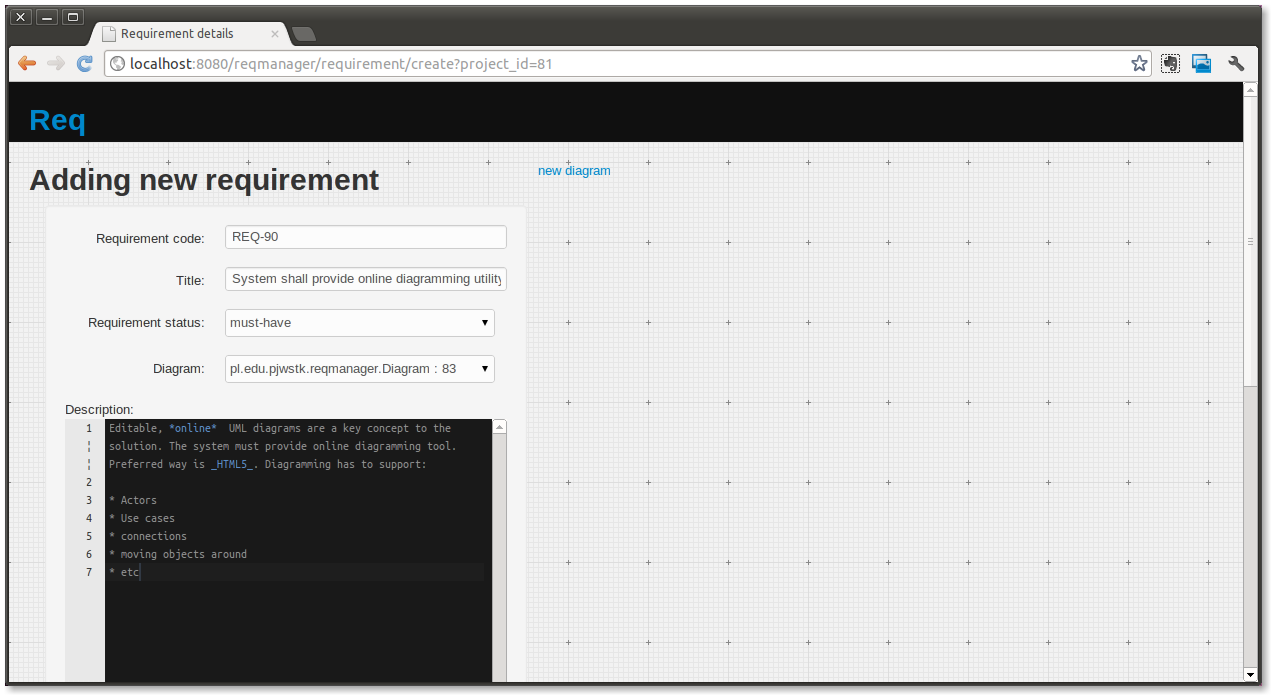
\includegraphics[width=1.0\textwidth]{img/tut_8.png}
        \caption{Współdzielenie diagramu}
        \label{fig:diagReuse}
      \end{figure*}

    \subsection{Łączenie przypadków użycia z wymaganiem}

      Wracając do widoku przedstawionego na Rysunku \ref{fig:addReq}, należy zwrócić uwagę na przycisk ,,mark for requirement'' w pasku narzędzi edytora UML. Wybierając tę opcję, a następnie wskazując wybrany przypadek użycia na diagramie, zostaje wykonana asynchronicznie operacja połączenia use case'u z wymaganiem. Po przejściu do podglądu wymagania, przypisane do niego przypadki użycia są zaznaczane kolorem żółtym. Właściwość ta, została zaprezentowana odpowiednio na Rysunkach \ref{fig:reqShow1} oraz \ref{fig:reqShow2}.

      \begin{figure*}[t]
        \centering
        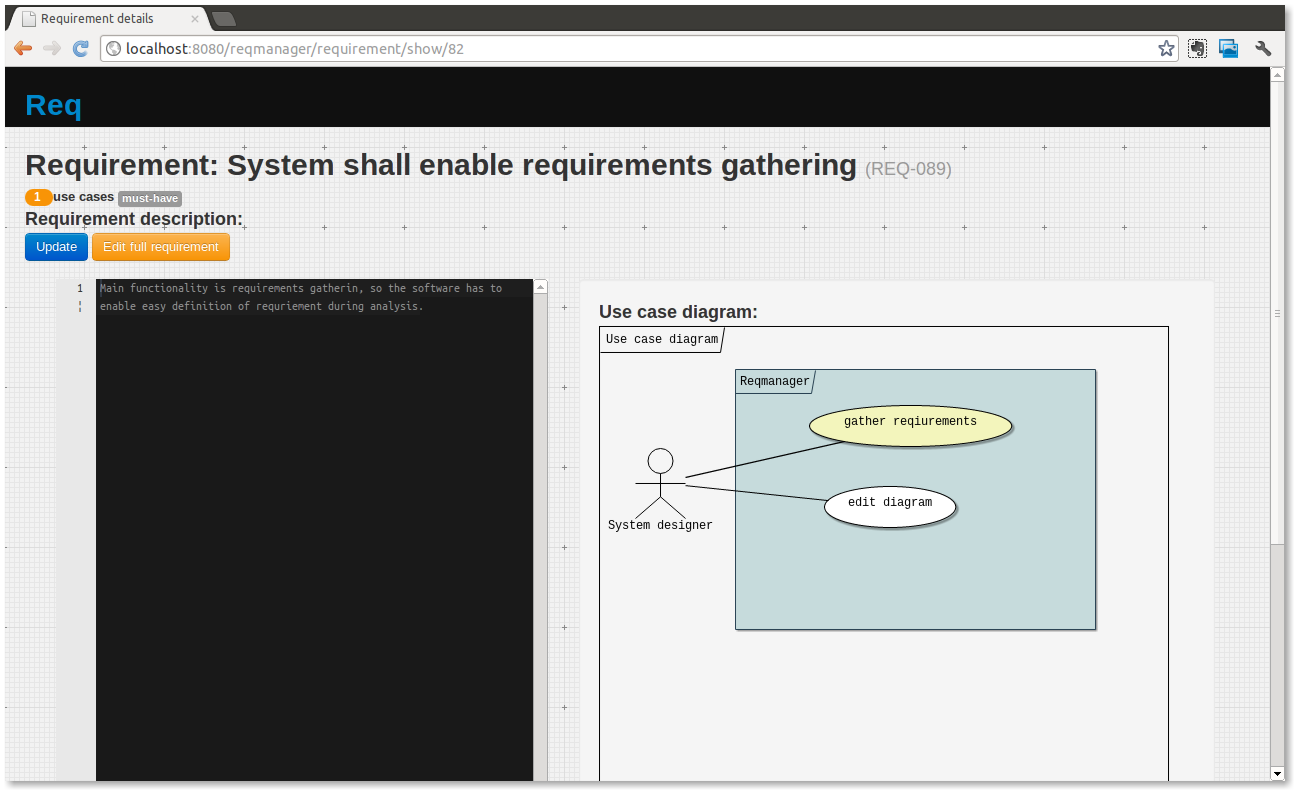
\includegraphics[width=1.0\textwidth]{img/tut_11.png}
        \caption{Jeden przypadek połączony z wymaganiem}
        \label{fig:reqShow1}
      \end{figure*}
      \begin{figure*}[t]
        \centering
        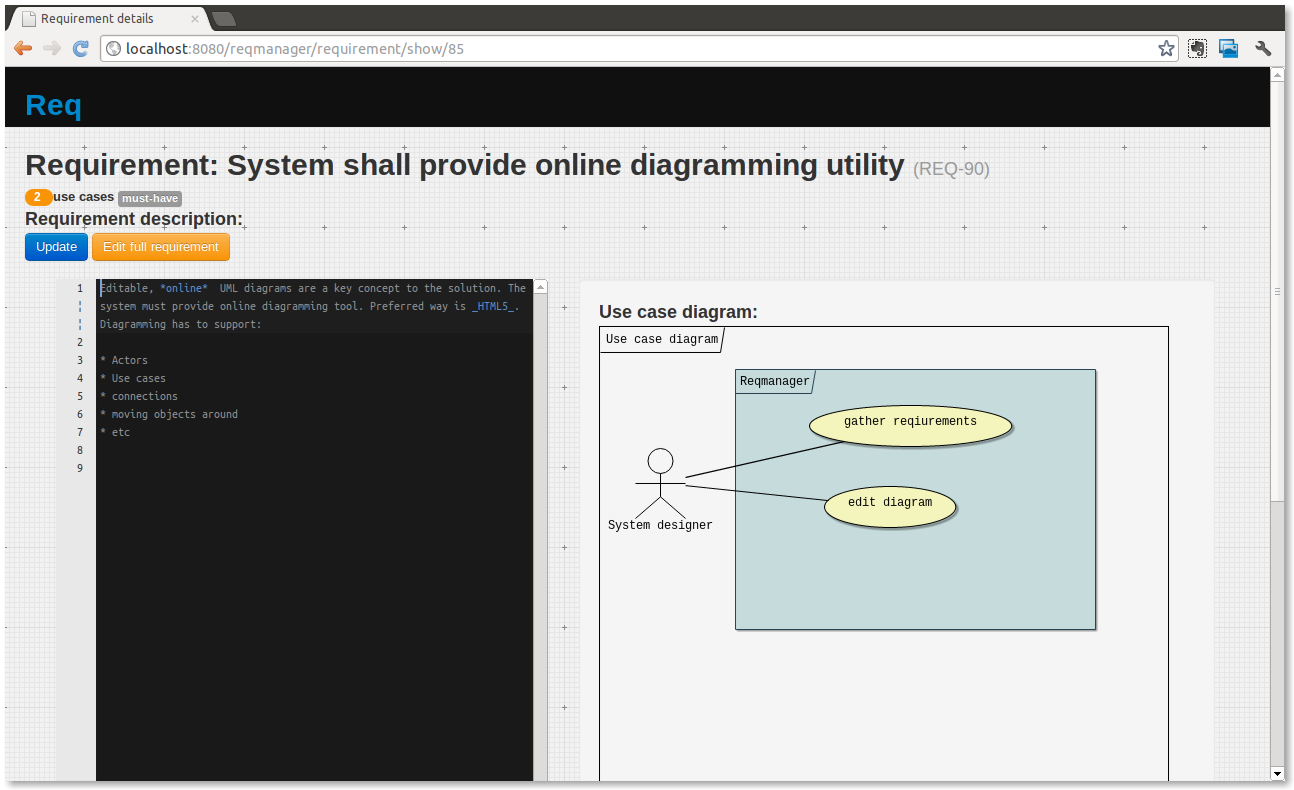
\includegraphics[width=1.0\textwidth]{img/tut_10.png}
        \caption{Dwa przypadki użycia połączone z wymaganiem}
        \label{fig:reqShow2}
      \end{figure*}

    \subsection{Generowanie specyfikacji}

      W każdym momencie prac nad analizą, użytkownicy mają możliwość wygenerowania aktualnej specyfikacji wymagań z ekranu głównego aplikacji. Proces polega wyłącznie na wybraniu opcji ,,Generate specification''. System analizuje dane wprowadzone do bazy i na ich podstawie generuje dokument PDF, który jest przekazywany do przeglądarki klienckiej. Wynik wygenerowania specyfikacji dla projektu powstałego na potrzeby powyższych przykładów pokazano na Rysunku \ref{fig:spec}.

      \begin{figure*}[t]
        \centering
        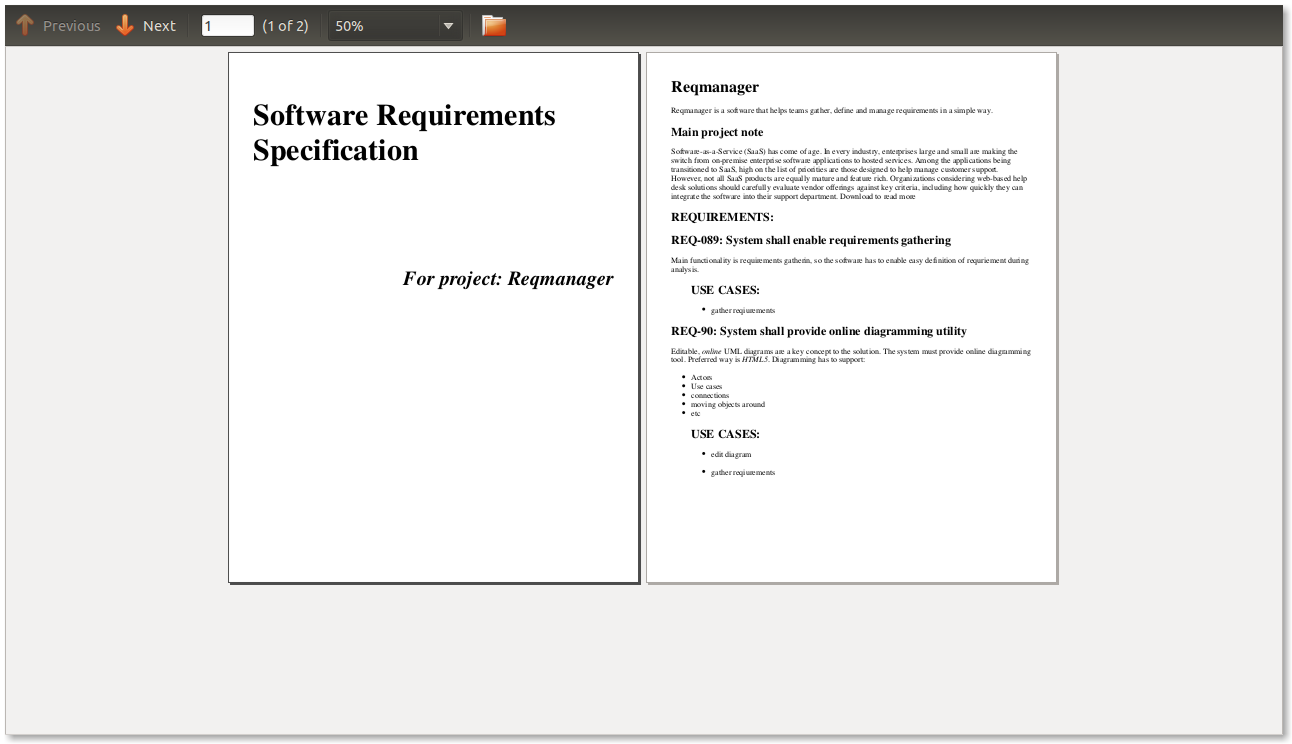
\includegraphics[width=1.0\textwidth]{img/tut_9.png}
        \caption{Wygenerowana specyfikacja wymagań w PDF}
        \label{fig:spec}
      \end{figure*}

  \newpage

  \section{Zalety i wady proponowanego rozwiązania}
    Proponowane rozwiązanie jest podjęciem próby uproszczenia procesów inżynierii wymagań. Głównym celem stworzenia prototypu było dostarczenie narzędzia umożliwiającego efektywne zbieranie i przetwarzanie wymagań przy jednoczesnym uproszczeniu poziomu jego skomplikowania. Powstał prototyp realizujący te cele, jednak siłą rzeczy, jest to narzędzie przystosowane jedynie do małych projektów. W przeciwieństwie do istniejących rozwiązań, filozofia proponowanego systemu inspirowana była filozofią systemów Unix - programy i aplikacje powinny wykonywać jedną czynność i powinny ją wykonywać możliwie najlepiej. Jednocześnie należy tworzyć aplikacje tak, aby mogły w łatwy sposób współpracować z innymi systemami. Dlatego proponowane rozwiązanie, aby rozwiązywało skutecznie problemy ogólnie pojętej inżynierii oprogramowania, powinno być stosowane komplementarnie z innymi narzędziami, w szczególności systemem zarządzania projektami i zespołem. Od świadomości i dojrzałości organizacji zależy, jak taka infrastruktura zostanie zbudowana oraz jak wybrane narzędzia będą funkcjonowały w organizacji.

    Dużą zaletą systemu jest dostępność przez przeglądarkę internetową przy jednoczesnej realizacji funkcjonalności manipulacji obiektami graficznymi. W szczególności zastosowanie technologii HTML5 daje przewagę w dostępności nad istniejącymi rozwiązaniami, najczęściej implementowanymi w technologii Flash. Rzadko też można spotkać podobny poziom elastyczności aplikacji do zarządzania wymaganiami. Koncepcja systemu celowo nie narzuca wielu ograniczeń związanych ze strukturą wymagań w wierze, że brak restrykcji projektanta wpłynie pozytywnie na proces definiowania i formułowania wymagań. 

    Sam wybór technologii jaką jest Grails, jest zaletą stworzonego prototypu. Zastosowanie tej technologii umożliwia łatwą rozbudowę i skalowanie systemu. System wtyczek platformy Grails sprzyja modułowej naturze aplikacji stworzonych w tej technologii. Z kolei zarządzający całą aplikacją ,,silnik'' oparty na String Framework, Hibernate ORM oraz filozofii ,,convention over configuration'' sprzyjają stosowaniu najlepszych praktyk programistycznych i ponowne wykorzystanie kodu.

    Z pewnością istotną wadą jest brak obsługi ,,śledzenia'' wymagań (traceability). Jednak w istniejących rozwiązaniach śledzenie wymagań nie rozwiązuje w pełni problemu. Nadal należy dbać o zgodność kodów i identyfikatorów wymagań w komunikacji z wieloma systemami. W dobrze zorganizowanej firmie, te problemy można wyeliminować przez narzucenie odpowiedniej kultury pracy, dbałość o szczegóły i skrupulatność w raportowaniu implementowanych rozwiązań do różnych systemów, jednak dopóki istnieje wiele narzędzi wspomagających różne etapy w procesie wytwórczym, odpowiednia komunikacja i wymiana danych jest jedyną metodą umożliwiającą skuteczne śledzenie wymagań.

  \chapter{Podsumowanie}
  
  W poprzednim rozdziale omówiono szczegóły implementacyjne przyjętego rozwiązania oraz krótko omówiono jego wady i zalety z perspektywy autora. Ten rozdział zawiera proponowane ścieżki rozwoju stworzonego oprogramowania oraz podsumowanie całości pracy.

  \section{Plan rozwoju}
  
    Proponowane narzędzie wsparcia gromadzenia wymagań, jest jedynie próbą nadania kierunku rozwojowi oprogramowania z tego segmentu. W pełni funkcjonalne narzędzie powinno wspierać obsługę wielu kont użytkowników, śledzenie wymagań, pełną obsługę diagramów (aktorzy, połączenia przypadków użycia, dziedziczenie), wsparcie importu/eksportu danych oraz automatyczny, asynchroniczny zapis obszaru roboczego diagramu. 
    
    Na szczególną uwagę zasługuje koncepcja integracji narzędzia z systemem kontroli wersji. Programista pracujący nad kodem źródłowym dotyczącym wybranego wymagania, mógłby w komentarzu zamykającym zadanie umieszczać identyfikator zrealizowanego wymagania. W systemie Reqmanager należałoby zaimplementować podsystem monitorujący wszystkie operacje zapisu do repozytorium, ekstrahować z komentarzy identyfikatory wymagań i odpowiednio oznaczać status ich realizacji na podstawie treści komentarza, umieszczając przy wymaganiu informacje z systemu kontroli wersji (programista, komentarz, data, status, etc).

    Kolejną możliwością rozwoju jest lepsze wsparcie dokumentowania przypadków użycia poprzez wzbogacenie możliwości edycji warunków zajścia a priori i a posteriori. Przykładowo warunki takie mogłyby być zapisywane w postaci kodu źródłowego Groovy lub Java i wykonywane po stronie serwera w odpowiednim momencie. Taka funkcjonalność umożliwiałaby nowatorskie podejście do testowania systemów oraz mogłaby dawać początek kierunku rozwoju bardziej zaawansowanego systemu umożliwiającego dynamiczne generowanie kodu poprzez definicję samych wymagań.

    Interesującą koncepcją jest również procesowanie języka naturalnego i automatyczna ekstrakcja wymagań z dokumentów tekstowych. Takie rozwiązanie musiałoby opierać się o zaawansowane biblioteki analizujące tekst oraz implementację inteligentnych algorytmów radzących sobie z ekstrakcją najistotniejszych fragmentów tekstu w celu sformułowania logicznego wymagania.

    
  \section{Zakończenie}

    Analiza istniejących rozwiązań, doświadczenia wyniesione z licznych, małych projektów komercyjnych realizowanych przez sektor MŚP oraz badania naukowe w tej dziedzinie, pokazują, że inżynieria wymagań jest w większości organizacji bardzo słabo rozwinięta. Jednak poziom skomplikowania procesorow i sprzętu komputerowego będzie rozwijał się w zatrważającym tempie jeszcze przez wiele lat, a wraz z nimi, potrzeba tworzenia coraz bardziej złożonego, niezawodnego oprogramowania. Dlatego organizacje chcące przetrwać na tak konkurencyjnym rynku jakim jest wytwarzanie oprogramowania, muszą pracować nad ciągłym usprawnianiem procesów, budową odpowiedniej infrastruktury i świadomości wśród pracowników oraz pracować blisko ze środowiskiem naukowym w poszukiwaniu coraz lepszych rozwiązań inżynieryjnych. Jedno narzędzie czy koncepcja nie rozwiąże problemów z jakimi mamy do czynienia w inżynierii wymagań. Jest to dziedzina integrująca bardzo zróżnicowane środowiska - świat naukowy i techniczny, ze światem biznesowym, opartym często na bardzo ciężko mierzalnych parametrach. Z tego względu niezwykle trudno jest wyznaczyć jasne granice inżynierii wymagań i odpowiednio sformalizować procesy. Być może w przyszłości, zostaną rozwinięte zaawansowane metody formalne pozyskiwania wymagań lub powstaną systemy procesowania języka naturalnego, które dadzą początek znacznyn przemianom i zniwelują zależność od czynnika ludzkiego w procesach wytwórzczych. 

    Od formalnego wprowadzenia dziedziny inżynierii oprogramowania, jako dziedziny nauki, w roku 1968, na konferencji NATO, wypracowano wiele skutecznych metod wspierającyych procesy związane z pozyskiwaniem, przetwarzaniem i zarządzaniem wymaganiami. Dojrzałość organizacji tworzących oprogramowanie zależy między innymi od poziomu wiedzy związanej z procesami inżynierii wymagań oraz umiejętności ich skutecznego wdrożenia. Narzędzia zastosowane w tych procesach grają istotną, jednak nie pierwszoplanową rolę. Nadal na dzień dzisiejszy kluczem do sukcesu projektu, oprócz odpowiedniego przygotowania merytorycznego jest umiejętność zbudowania odpowiedniego zespołu specjalistów z doświadczeniem i wyposażenie ich w odpowiednie mechanizmy pozwalające na swobodne i efektywne działanie. Organizacje nadal starające się przełożyć bezpośrednio dziedzinę wytwarzania oprogramowania na klasyczne zasady inżynierii systemów zdają się niedostrzegać lub ignorować drastyczne różnice jakie dzielą te dziedziny. Kluczem do sukcesu projektów informatycznych, w pierwszej kolejności, są doskonali, doświadczeni projektanci.

\blacksquare


  \printbibliography
\end{document}
